The output of a multivariate algorithm is used as the final discriminant for the signal extraction for both the di-Higgs and the leptoquark-pair analyses, as described in Section~\ref{sec:fit} and Section~\ref{sec:fitLQ}. 

The di-Higgs non-resonant SM signal is well-defined in its kinematic properties, and so a boosted decision tree (neural network) trained on this signal is used in the \hadhad (\lephad) channel. 

The di-Higgs resonant signal and the leptoquark-pair signal, however, is not a single signal hypothesis, but rather a set of continuous signal hypotheses parameterised by the mass of the heavy resonance which decays to Higgs boson pairs, or by the mass of the leptoquarks which decay into the $b-\tau$ pairs. For these cases, a standard binary classification algorithm is not optimal. A set of single discriminants trained on each of the simulated signal hypotheses would provide good discrimination for the simulated hypotheses, but can not interpolate well between these points. For this reason, and to reduce the number of algorithms that require training, Parametric Neural Networks (PNNs)~\cite{Baldi:2016fzo} are used for the extraction of the resonant signal. PNNs are neural networks which enable optimal signal-to-background classification for signal spectra connected by one or more physics parameters. As this problem is a smoothly-varying learning task, the PNN is not just able to learn how to classify signals at the simulated signal mass training points, but also how to interpolate between them. Tests of these properties are described in Appendix~\ref{sec:appendix_pnn_HH}.

The PNNs used in the analyses described in this note take as an input parameter to specify which signal should be targeted, along side the feature variables, the heavy resonance mass for the di-Higgs analysis and the leptoquark mass for the leptoquark-pair analysis. During training, the PNNs are trained on all the signals simultaneously, and are provided with the generator-level masses of the signals and a random mass from the distribution of simulated signal masses for the background. The background events are provided with such distribution of simulated signal masses because the background events do not have a well-defined value for the "truth scalar resonance mass" and the "parameter" assigned to background events must be uninformative regarding the signal / background discrimination. This is achieved by randomly assigning a "truth scalar resonance mass" that follows the distribution seen in the signal training events. During implementation, the mass of the targeted signal is given, which results in optimal discrimination for that signal hypothesis. As the ideal neural network output (when trained on the binary cross entropy) is a monotonic function of the signal-to-background density ratio, this means that the PNN will optimally classify the targeted signal events, as specified by the physics input parameter.

For all trainings described in the following the input variables are "standardised" by subtracting the median and dividing by the interquartile range (Median / IQR due to better stability w.r.t. outliers compared to Mean / Stddev). The same offsets / scales are applied independently of the source / origin of the event (i.e. data, signal, background etc.). 


\subsection{di-Higgs}
\subsection{$\tau_{had}\tau_{had}$ channel}
\label{ssec:mva_hadhad}

In the di-Higgs $bb\tau_{had}\tau_{had}$ channel 5 variables are used as inputs in the training of the non-resonant SM BDT and of the resonant PNN:

\begin{itemize}
\item $m_{HH}$: The invariant mass of the di-Higgs system is reconstructed from the di-$\tau_{had}$ 4-momentum (calculated using MMC) and di-$b$-jet 4-momentum;
\item $m_{\tau\tau}^{MMC}$: The invariant mass of the di-$\tau$ system, calculated using the MMC;
\item $m_{bb}$: The invariant mass of the di-$b$-jet system;
\item $\Delta  R(\tau, \tau)$: The  $\Delta R$ between the visible-$\tau$ decay products;
\item $\Delta  R(b, b)$: The  $\Delta R$ between the two $b$-jets.
\end{itemize}

The BDT and the PNN are trained in the signal region against the sum
of all backgrounds weighted by their respective cross sections (the
\ttbar background is fully taken from the MC in the training,
including the component with fake \tauhad). The signal events for all
mass points are rescaled with weights to be equal and matching the
total background yield (for training only). The available training
statistics can be extracted from~\Cref{tab:HadHadYields} after
considering the split of the dataset into even- and odd-numbered
events\footnote{For the final training approximately 50\,\% of events
  in the preselection region are available. For the hyperparameter
  optimization only 40\,\% are used for training due to the 5-fold
  cross validation that is used (i.e.\
  $\frac{4}{5} \text{(CV)} \times \frac{1}{2} \text{(even-odd)} =
  40\,\%$) due to the fold that is held out for validation.}.

Figure~\ref{fig:HadHadPreselectionPNNInputsDistributions} shows the data/prediction comparison for the pre-fit MVA input variables distributions in the di-Higgs $bb\tau_{had}\tau_{had}$ signal region (these distributions are not blinded as the definition of the signal region selection is very loose as to define a pre-selection region and MVAs are then used in this region to separate background and signal).  Figures~\ref{fig:HadHadPreselectionPNNInputsDistributions2015}-~\ref{fig:HadHadPreselectionPNNInputsDistributions2018} show the same distributions split by data-taking period.

%\begin{figure}
%\centering
%\subfloat[]
%   {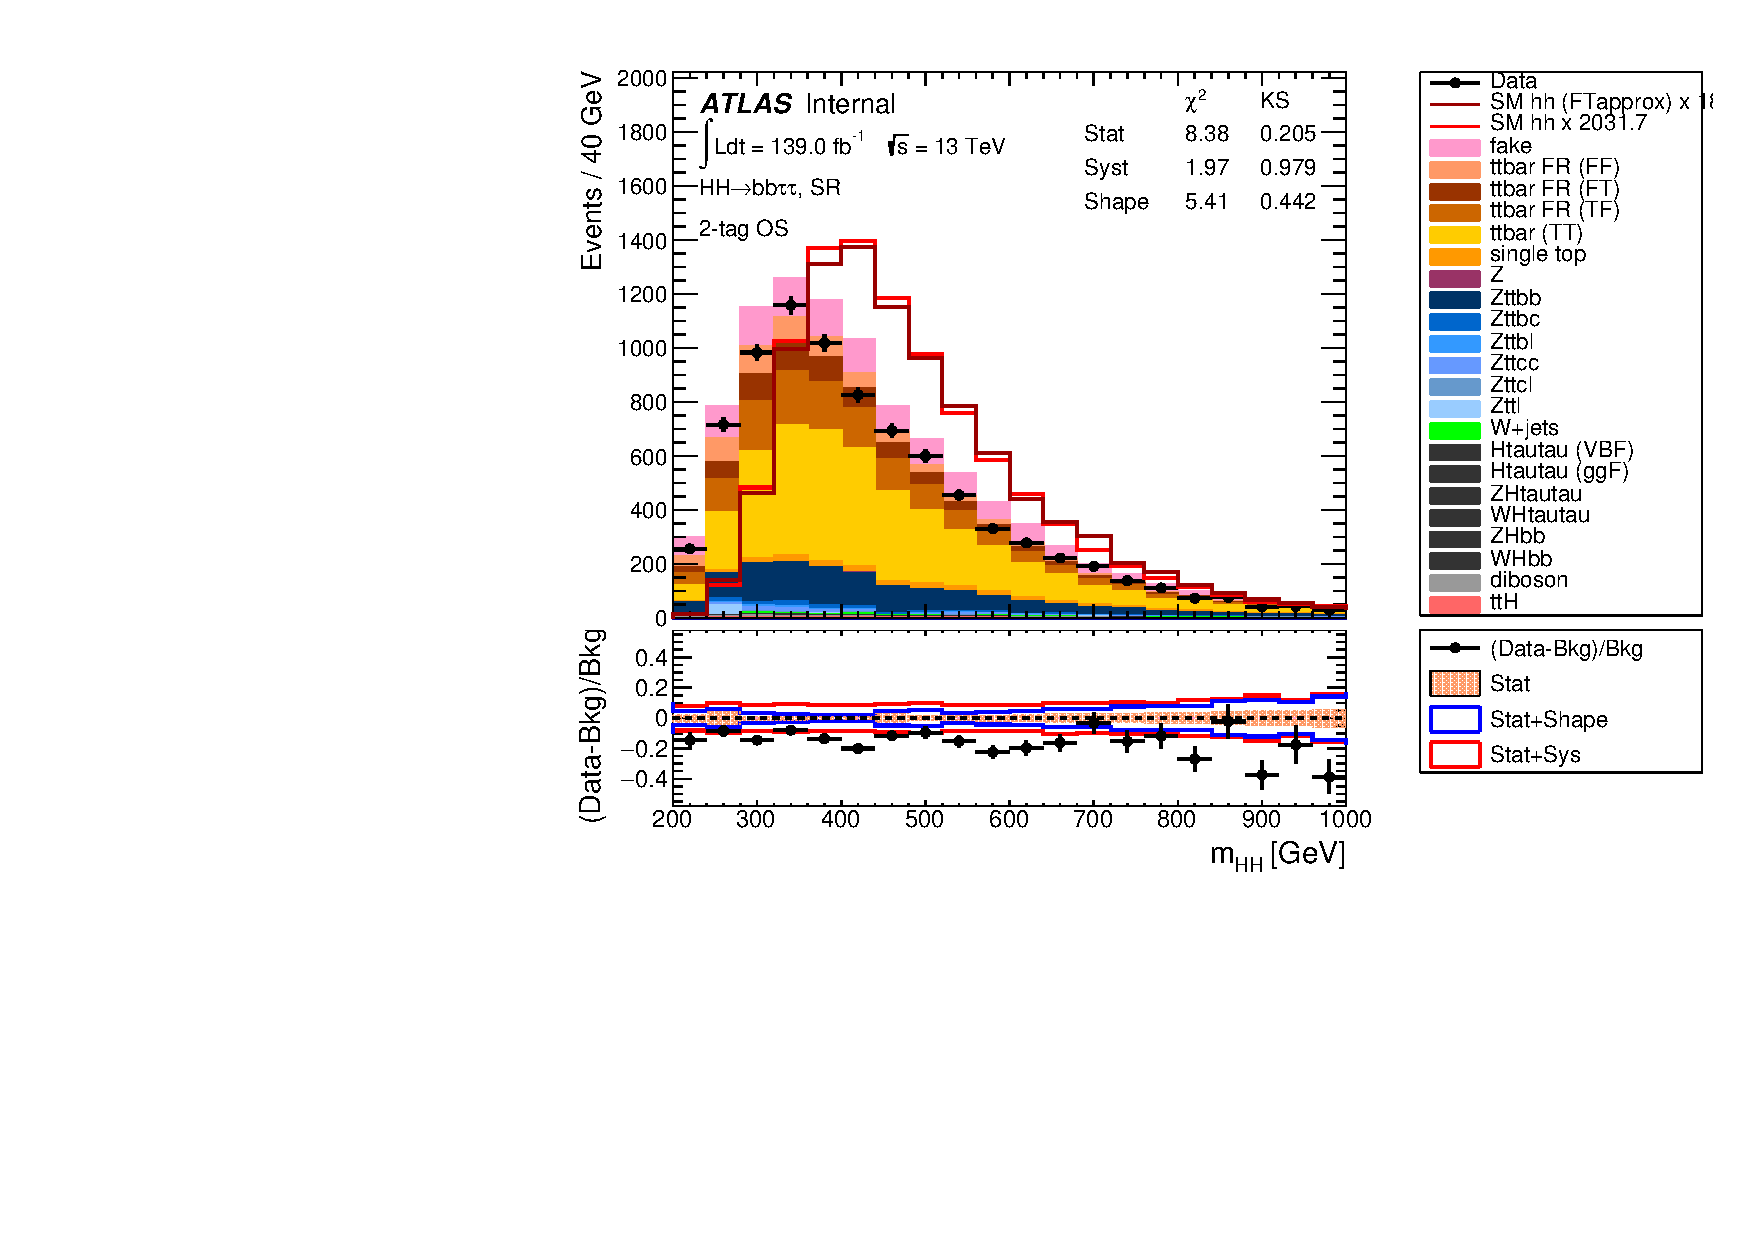
\includegraphics[width=.45\textwidth]{figures/mva/HH/HadHad/C_2tag2pjet_0ptv_LL_OS_mHH.pdf}}\quad
%\subfloat[]
%   {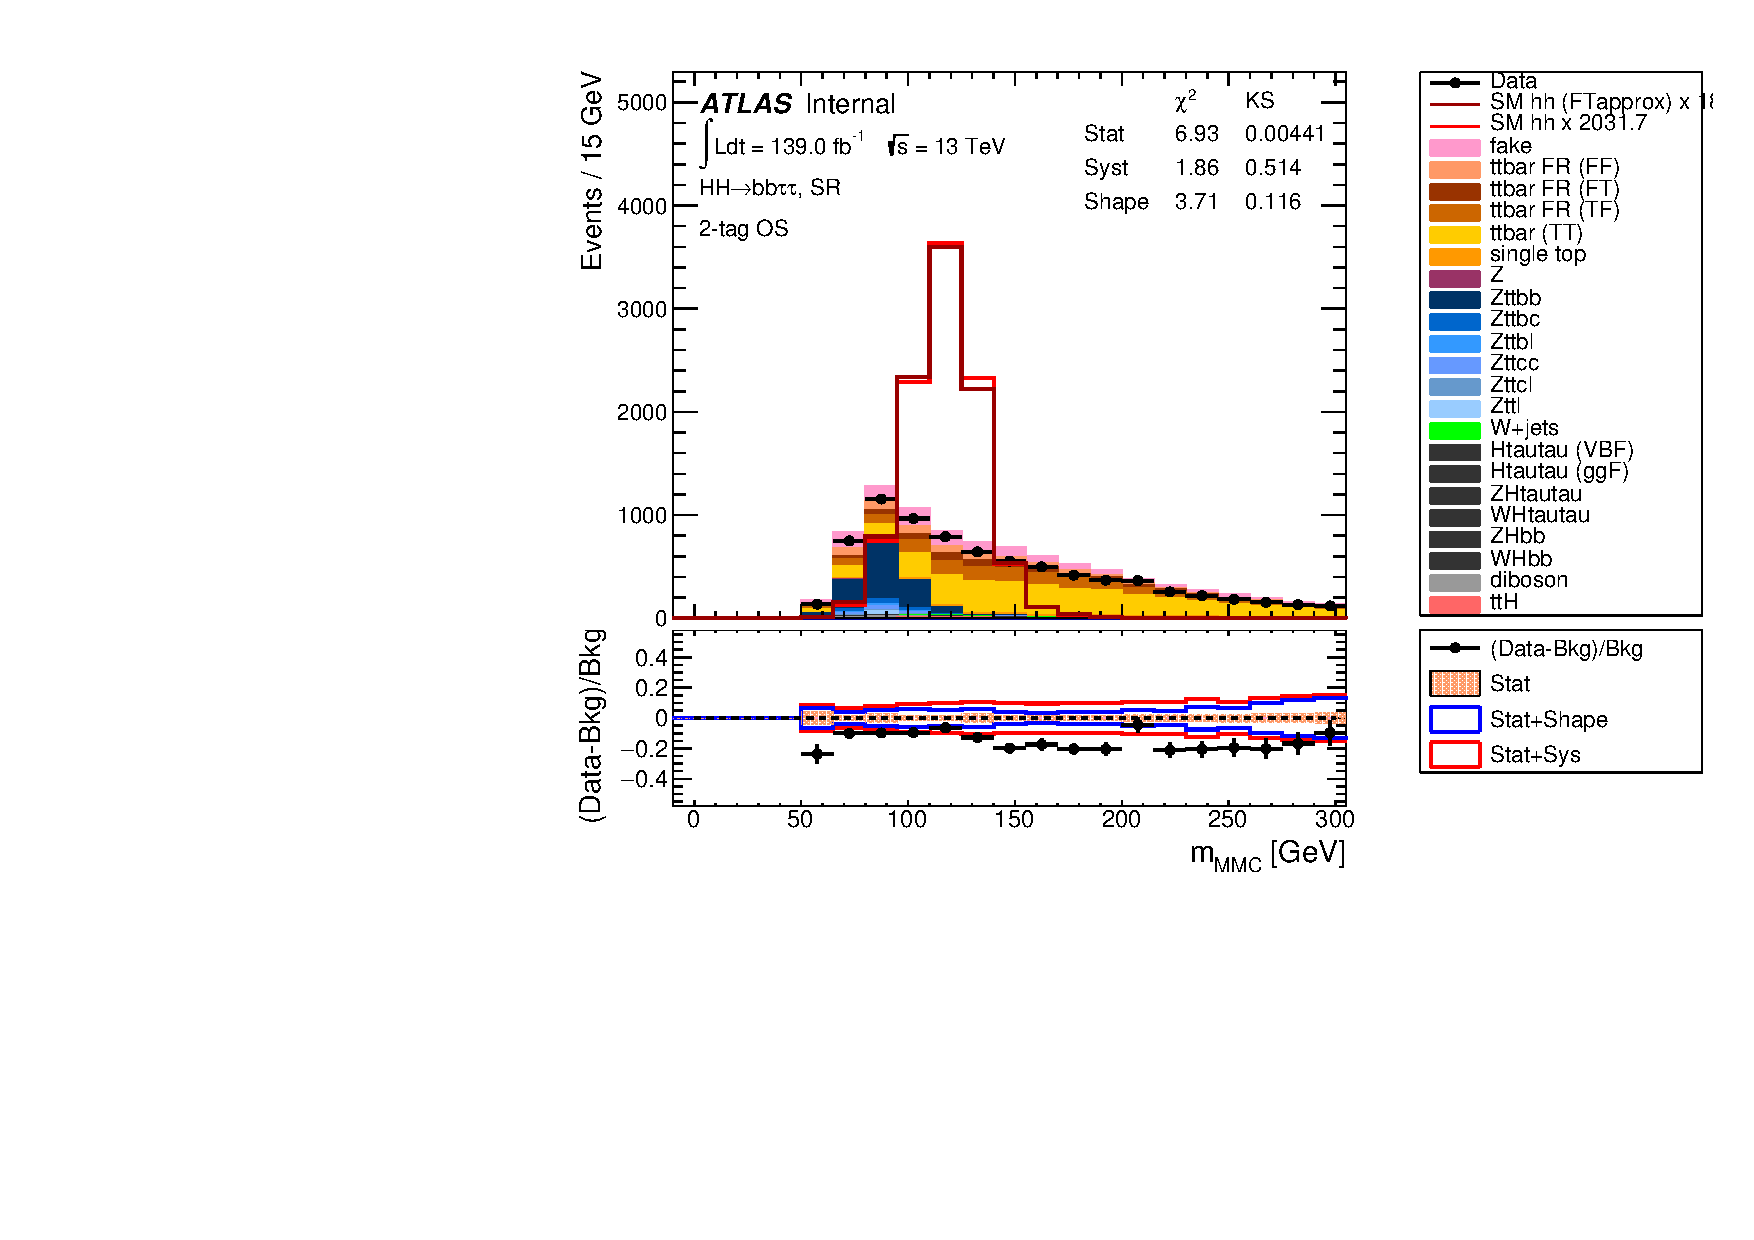
\includegraphics[width=.45\textwidth]{figures/mva/HH/HadHad/C_2tag2pjet_0ptv_LL_OS_mMMC.pdf}} \quad
%\subfloat[]
%   {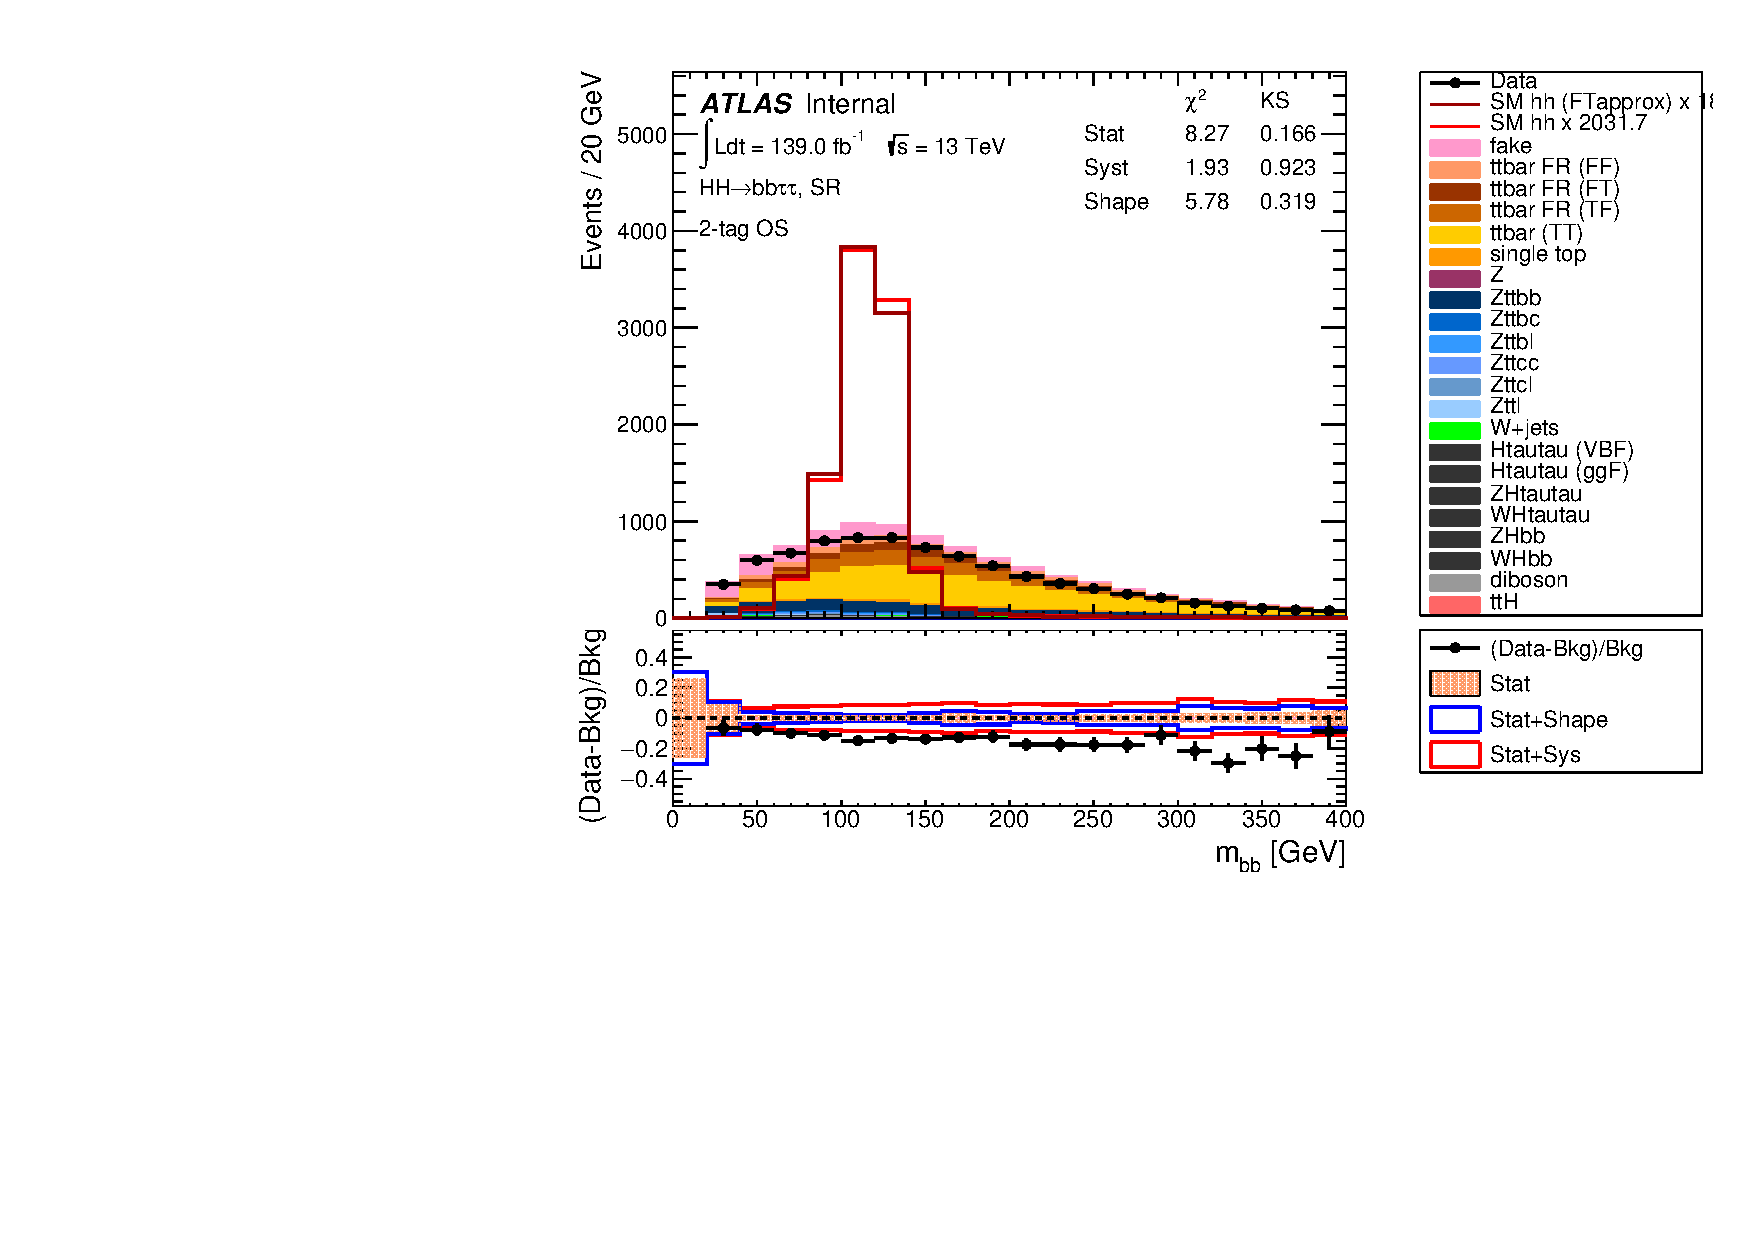
\includegraphics[width=.45\textwidth]{figures/mva/HH/HadHad/C_2tag2pjet_0ptv_LL_OS_mBB.pdf}}\quad
%\subfloat[]
%   {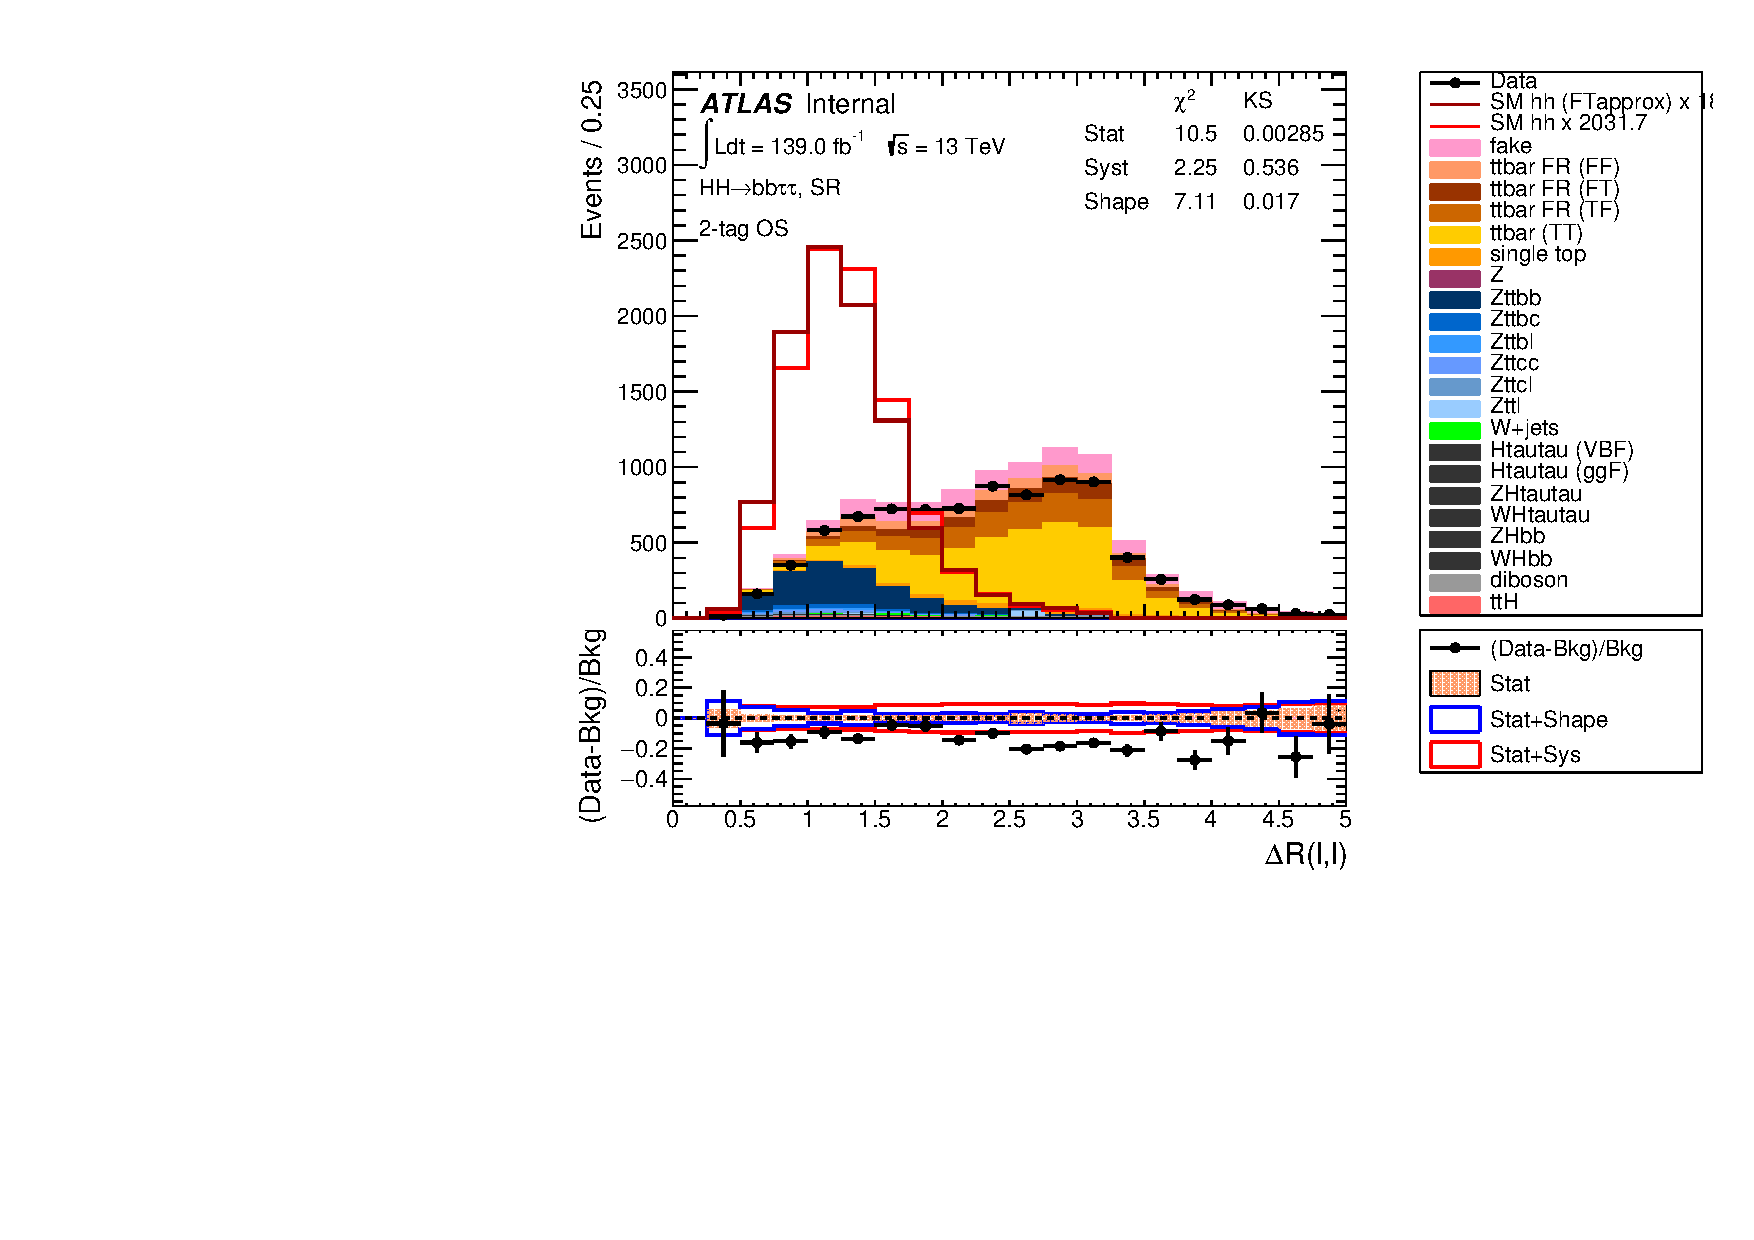
\includegraphics[width=.45\textwidth]{figures/mva/HH/HadHad/C_2tag2pjet_0ptv_LL_OS_dRTauTau.pdf}} \quad
%   \subfloat[]
%   {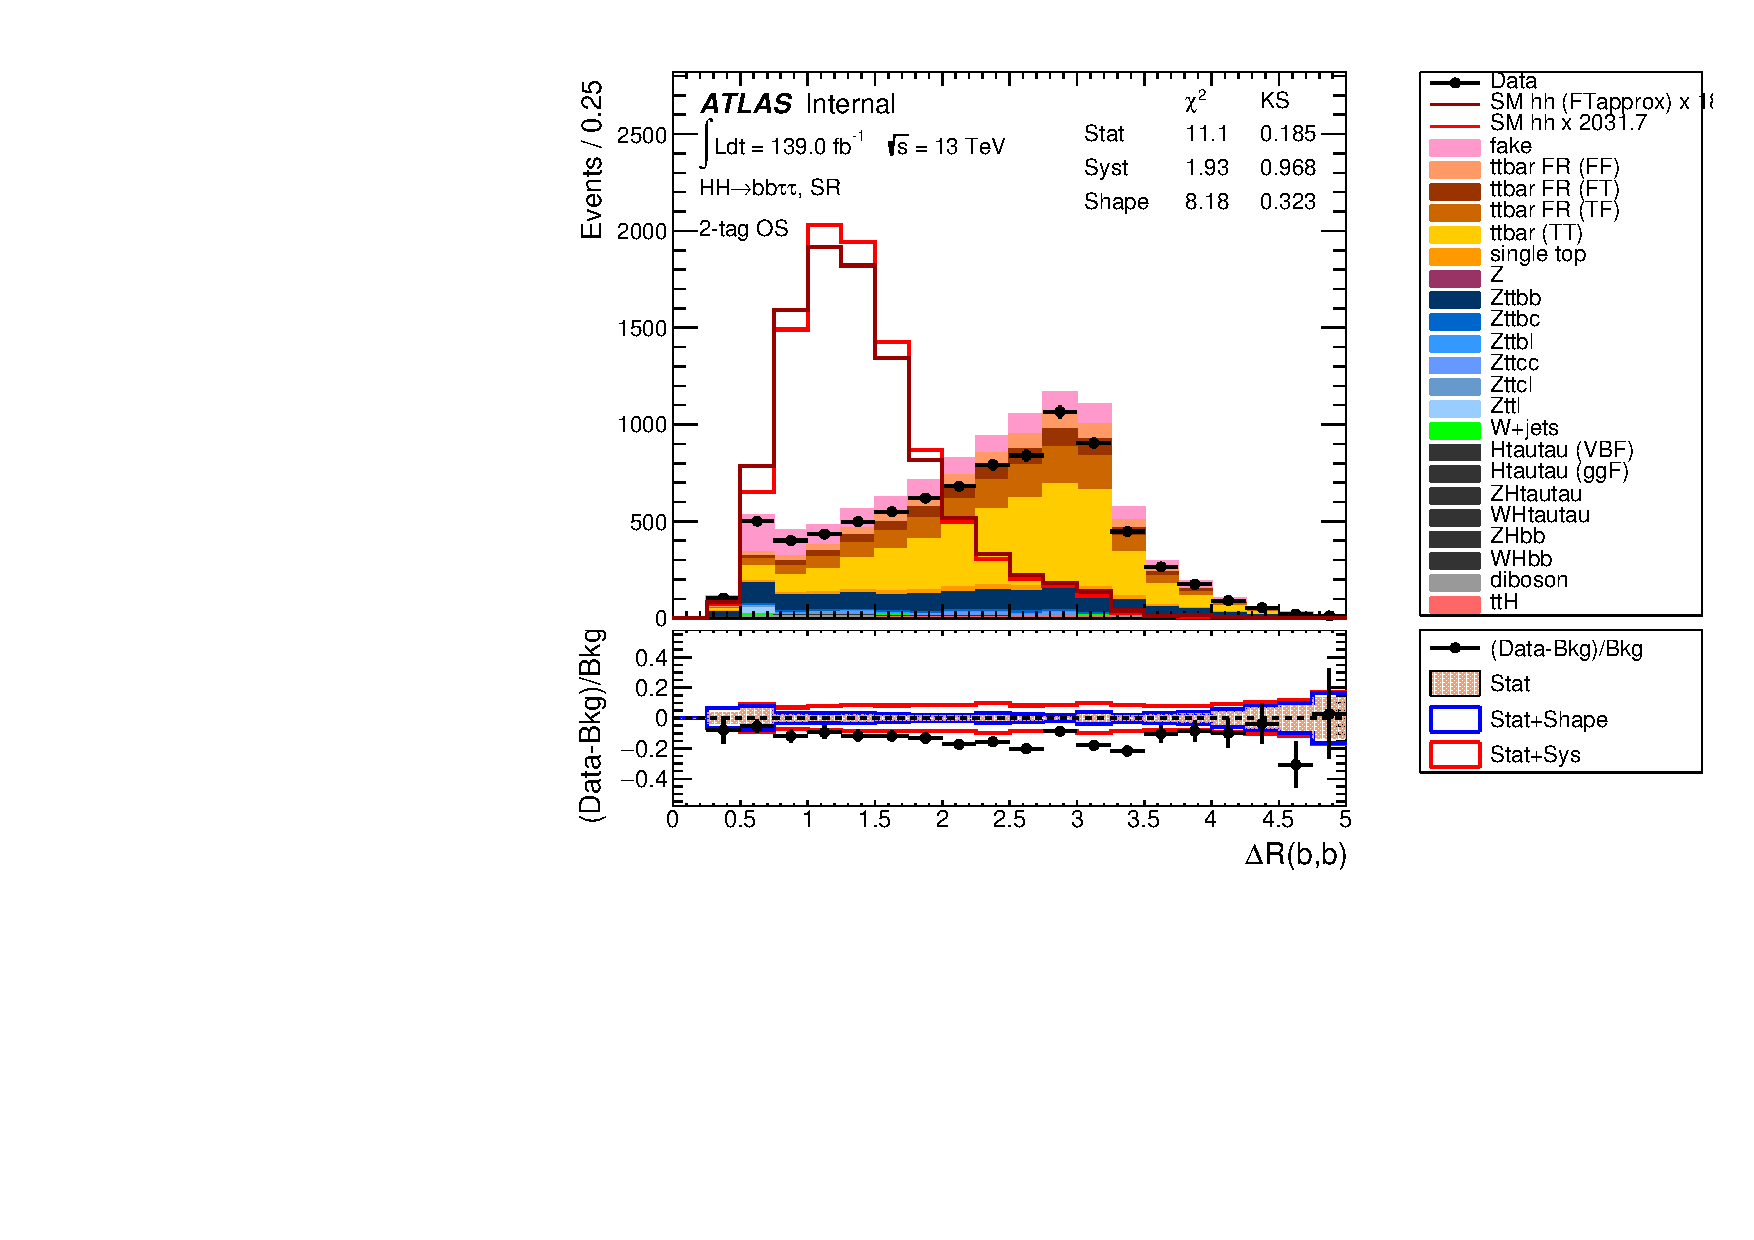
\includegraphics[width=.45\textwidth]{figures/mva/HH/HadHad/C_2tag2pjet_0ptv_LL_OS_dRBB.pdf}} \quad
%\caption{Pre-fit MVA input variable distributions in the di-Higgs
%  $bb\tau_{had}\tau_{had}$ signal region. The yields for Zttbb, Zttbc and Zttcc are scaled by 1.3. The uncertainty band includes CP uncertainties and $t\bar{t}$ and fake-$\tau_{had}$ backgrounds modelling uncertainties. (Inputs from 2020\_10\_16) (\textcolor{red}{To do: replace with plots from WSMaker including all uncertainties.})}
%\label{fig:HadHadPreselectionPNNInputsDistributions}
%\end{figure}

\begin{figure}
\centering
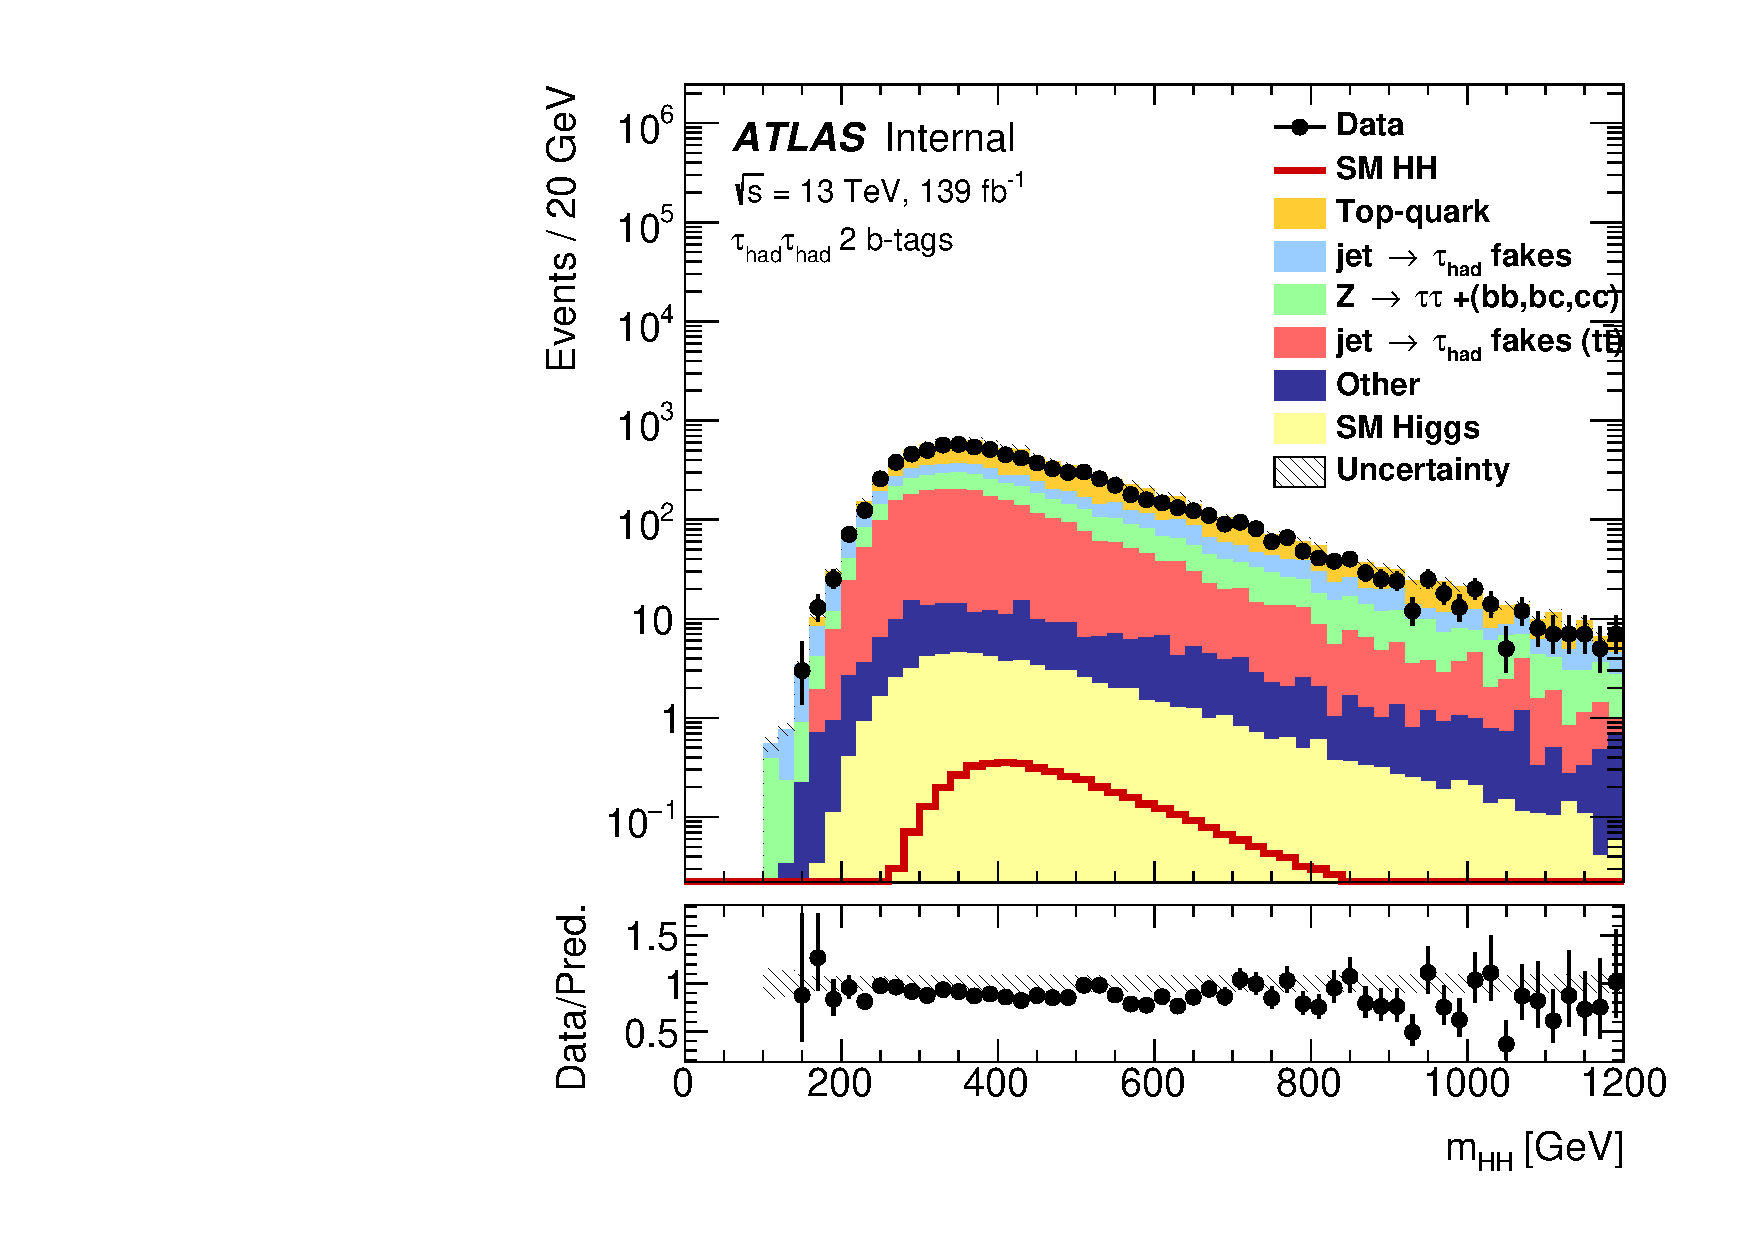
\includegraphics[width=.45\textwidth]{figures/mva/HH/HadHad/Region_BMin0_incJet1_distmHH_J2_Y2015_DLLOS_T2_SpcTauHH_L0_Prefitlog.pdf}
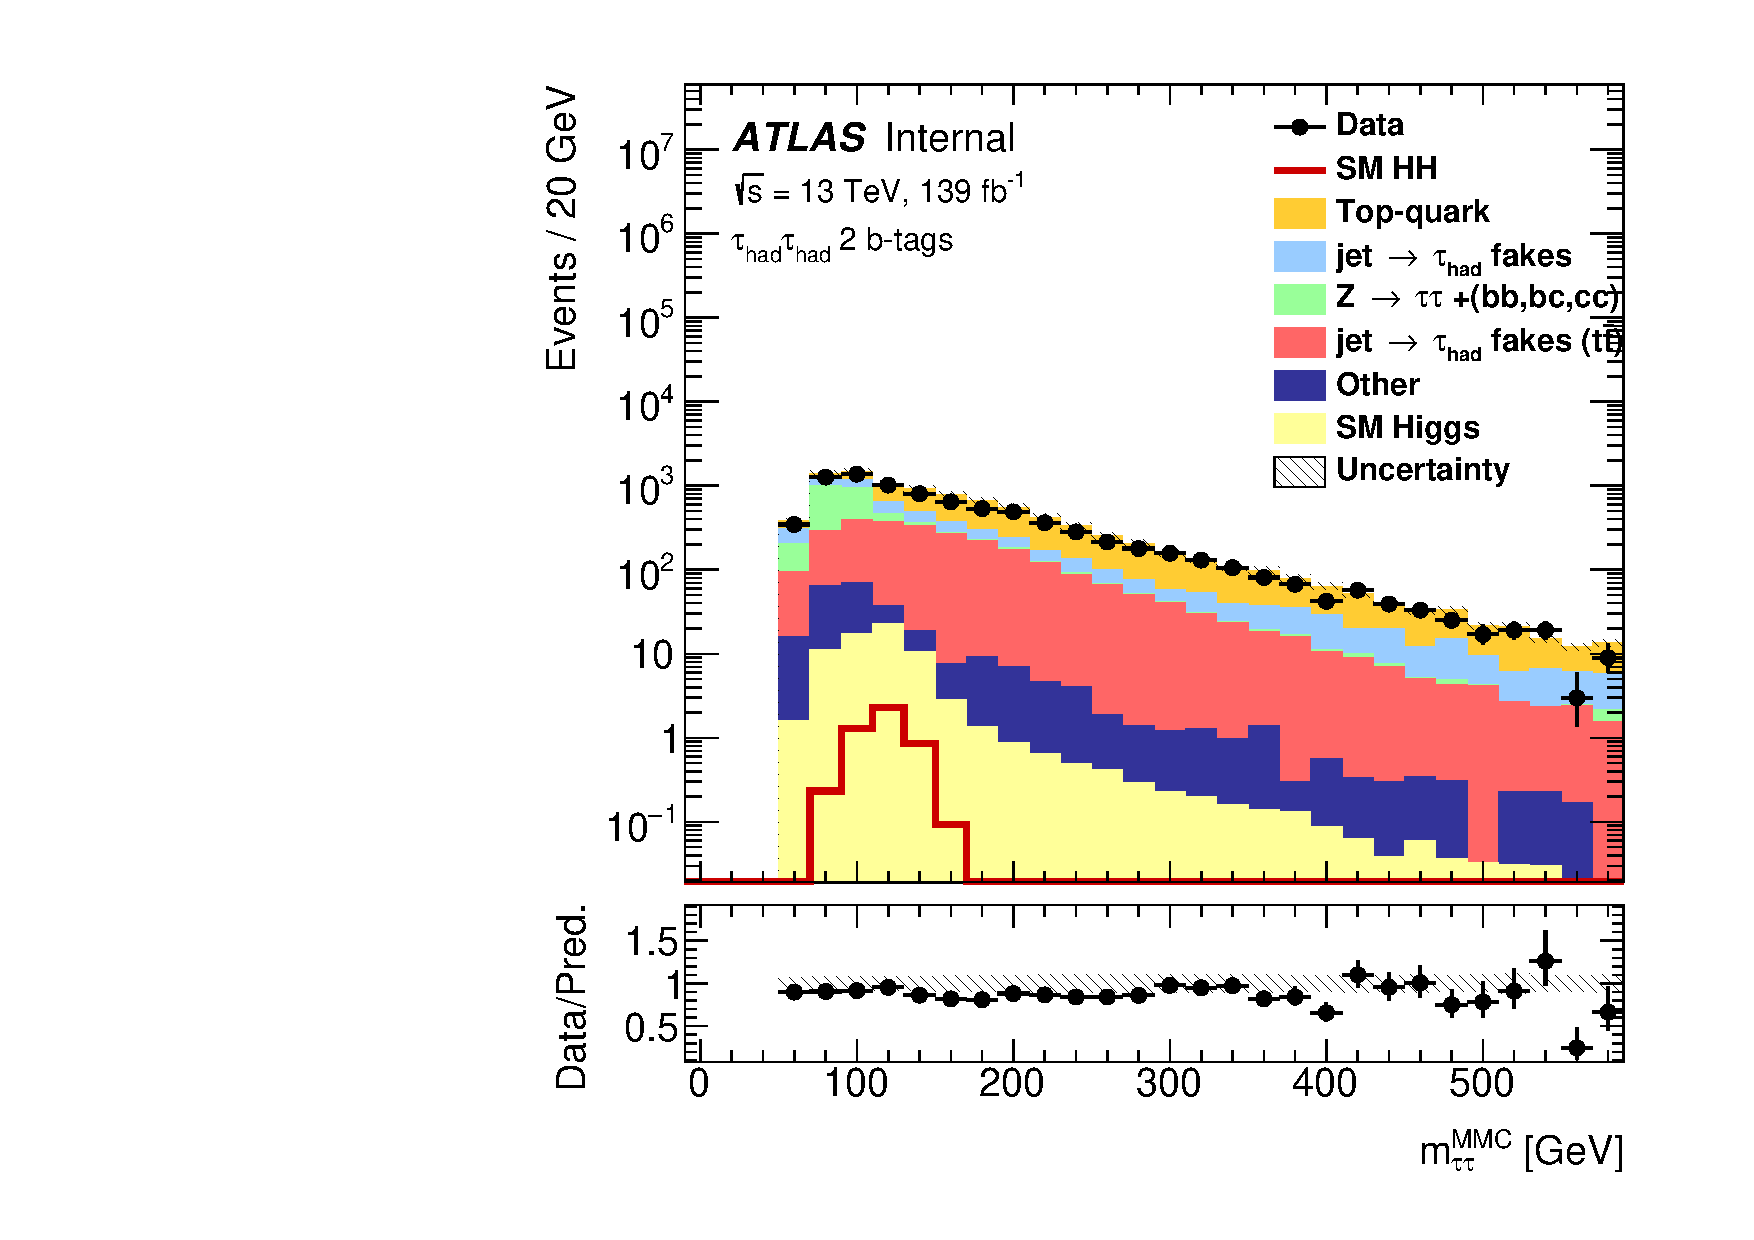
\includegraphics[width=.45\textwidth]{figures/mva/HH/HadHad/Region_BMin0_incJet1_distmMMC_J2_Y2015_DLLOS_T2_SpcTauHH_L0_Prefitlog.pdf}\\
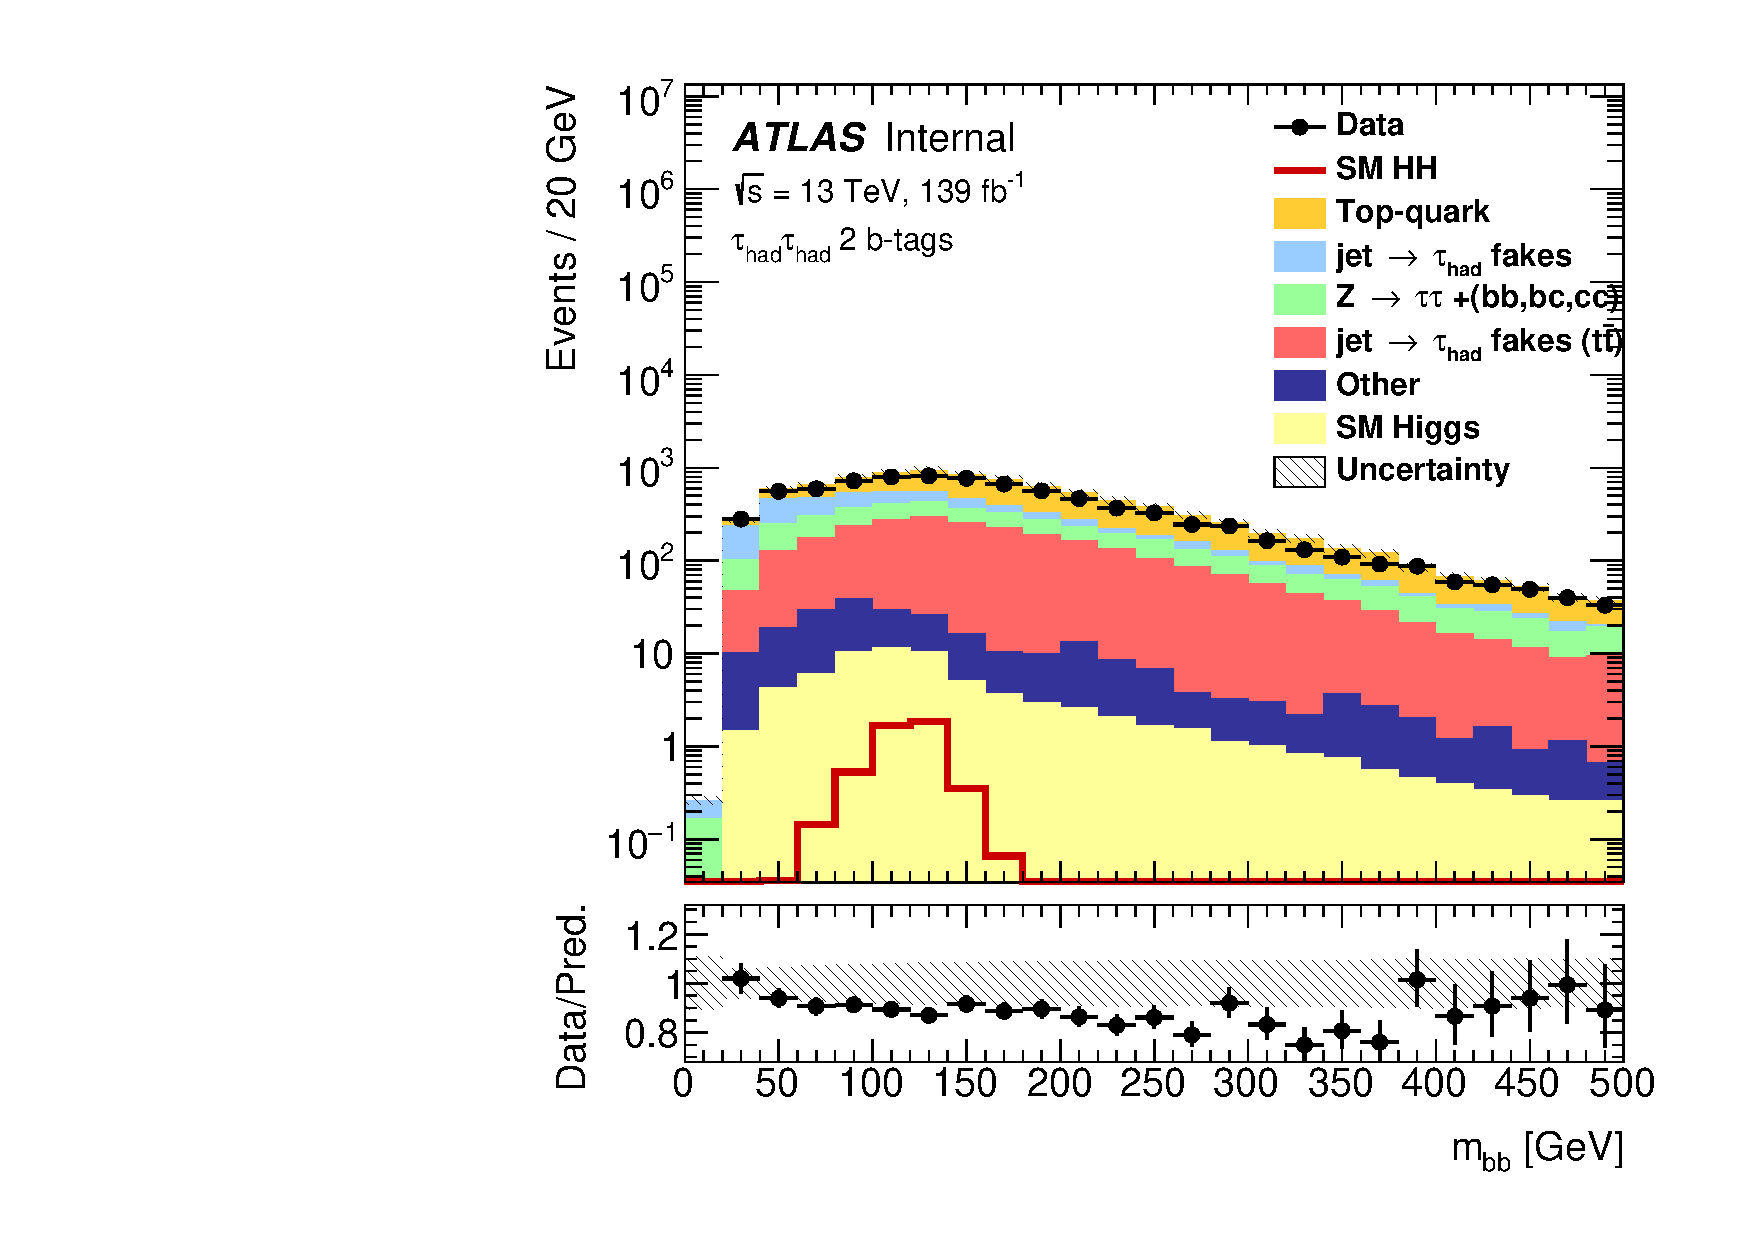
\includegraphics[width=.45\textwidth]{figures/mva/HH/HadHad/Region_BMin0_incJet1_distmBB_J2_Y2015_DLLOS_T2_SpcTauHH_L0_Prefitlog.pdf}
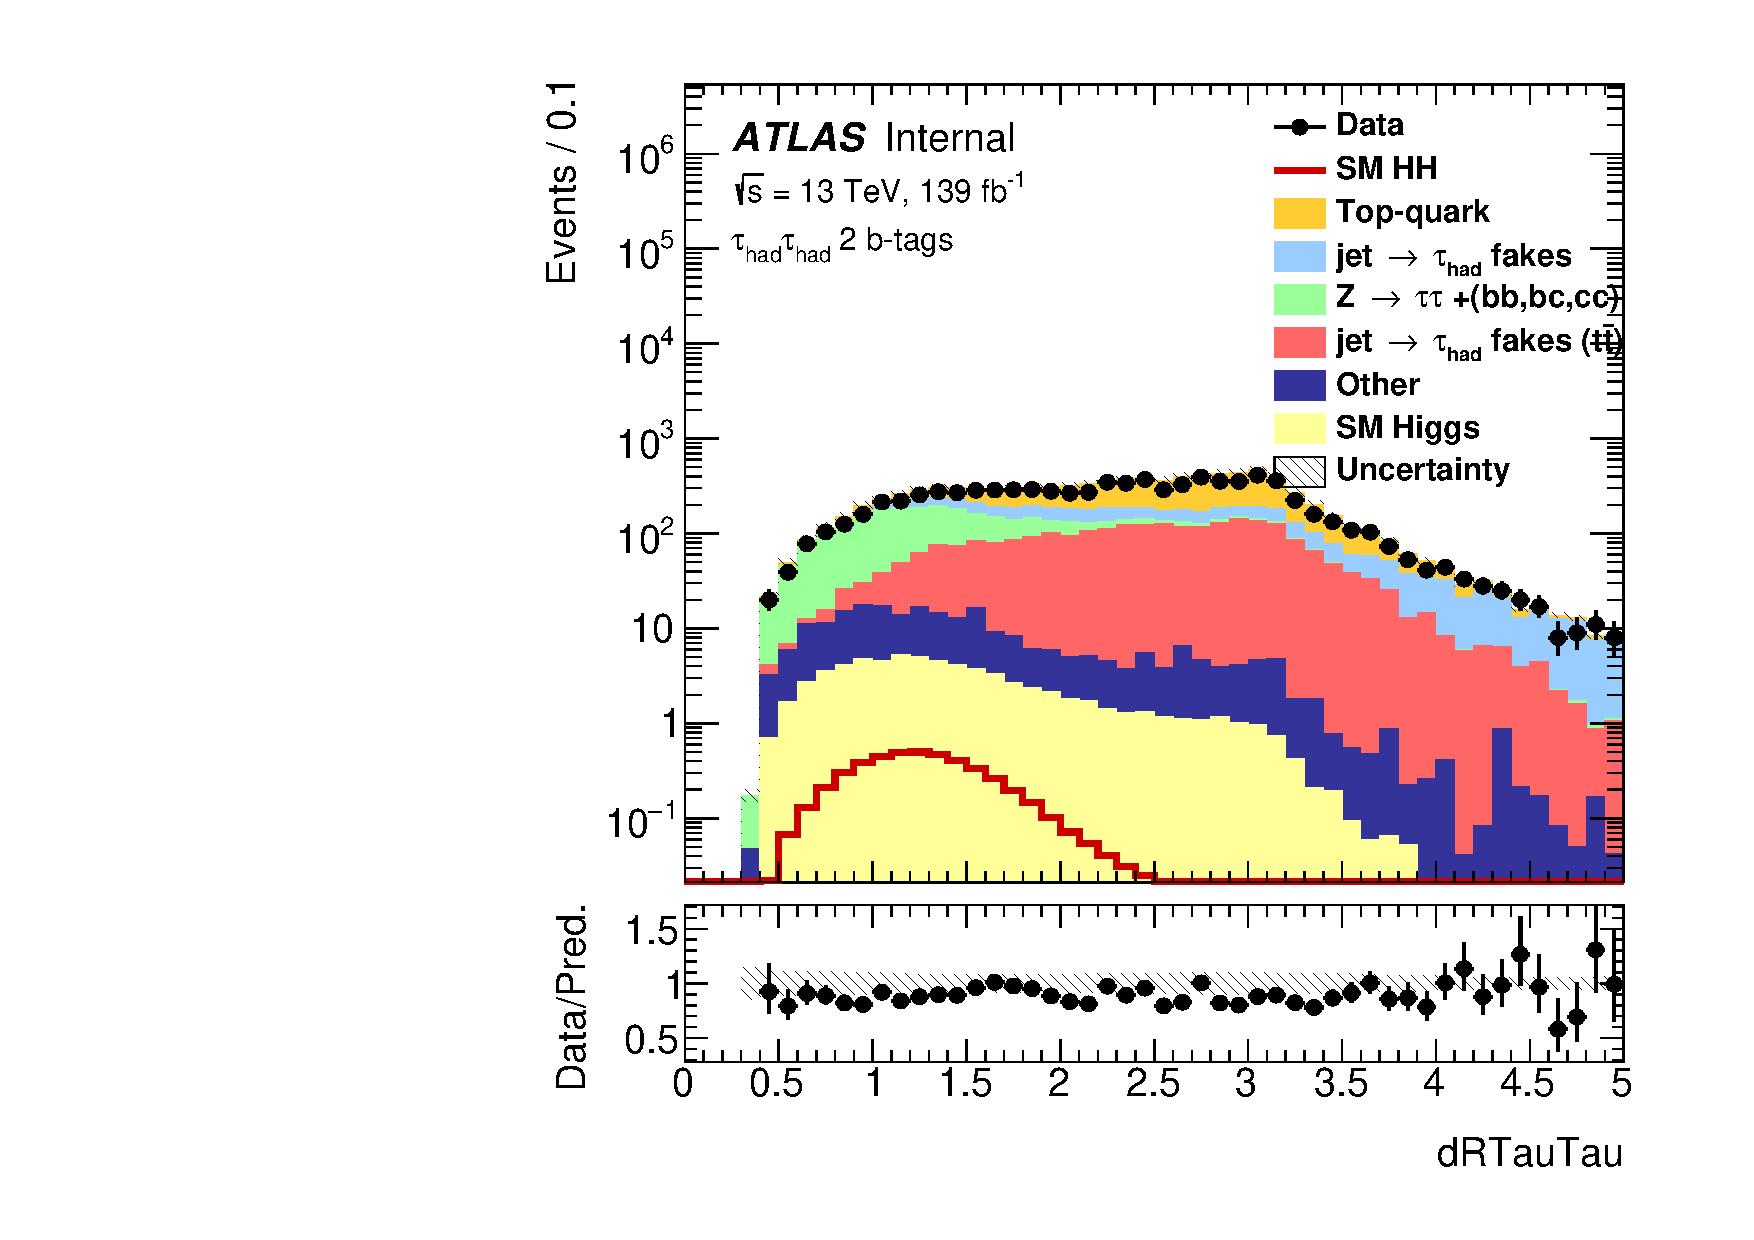
\includegraphics[width=.45\textwidth]{figures/mva/HH/HadHad/Region_BMin0_incJet1_distdRTauTau_J2_Y2015_DLLOS_T2_SpcTauHH_L0_Prefitlog.pdf}\\
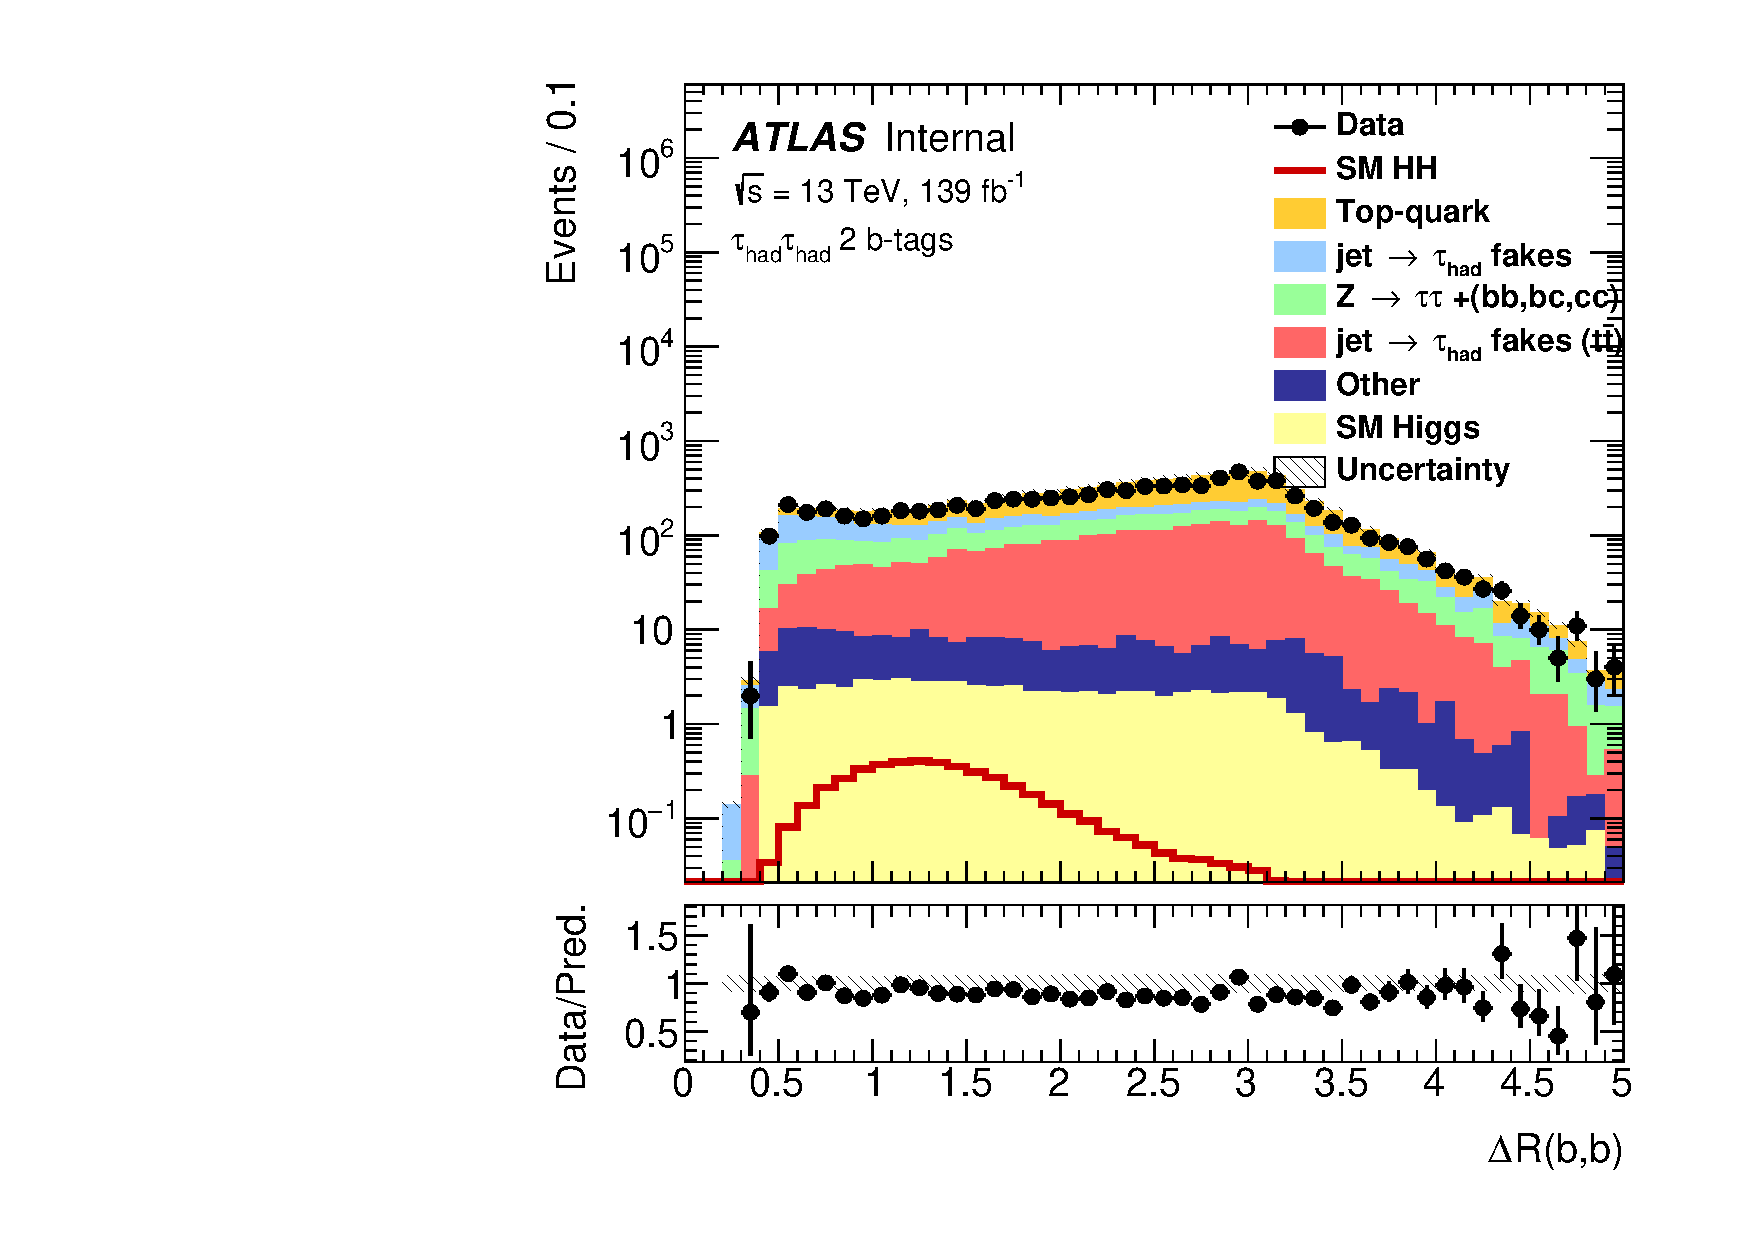
\includegraphics[width=.45\textwidth]{figures/mva/HH/HadHad/Region_BMin0_incJet1_distdRBB_J2_Y2015_DLLOS_T2_SpcTauHH_L0_Prefitlog.pdf}
\caption{Pre-fit MVA input variable distributions in the di-Higgs
  $bb\tau_{had}\tau_{had}$ signal region. The uncertainty band includes all uncertainties. The signal is normalised to the input cross section. (Inputs from 2021\_01\_15).}
\label{fig:HadHadPreselectionPNNInputsDistributions}
\end{figure}


\begin{figure}
\centering
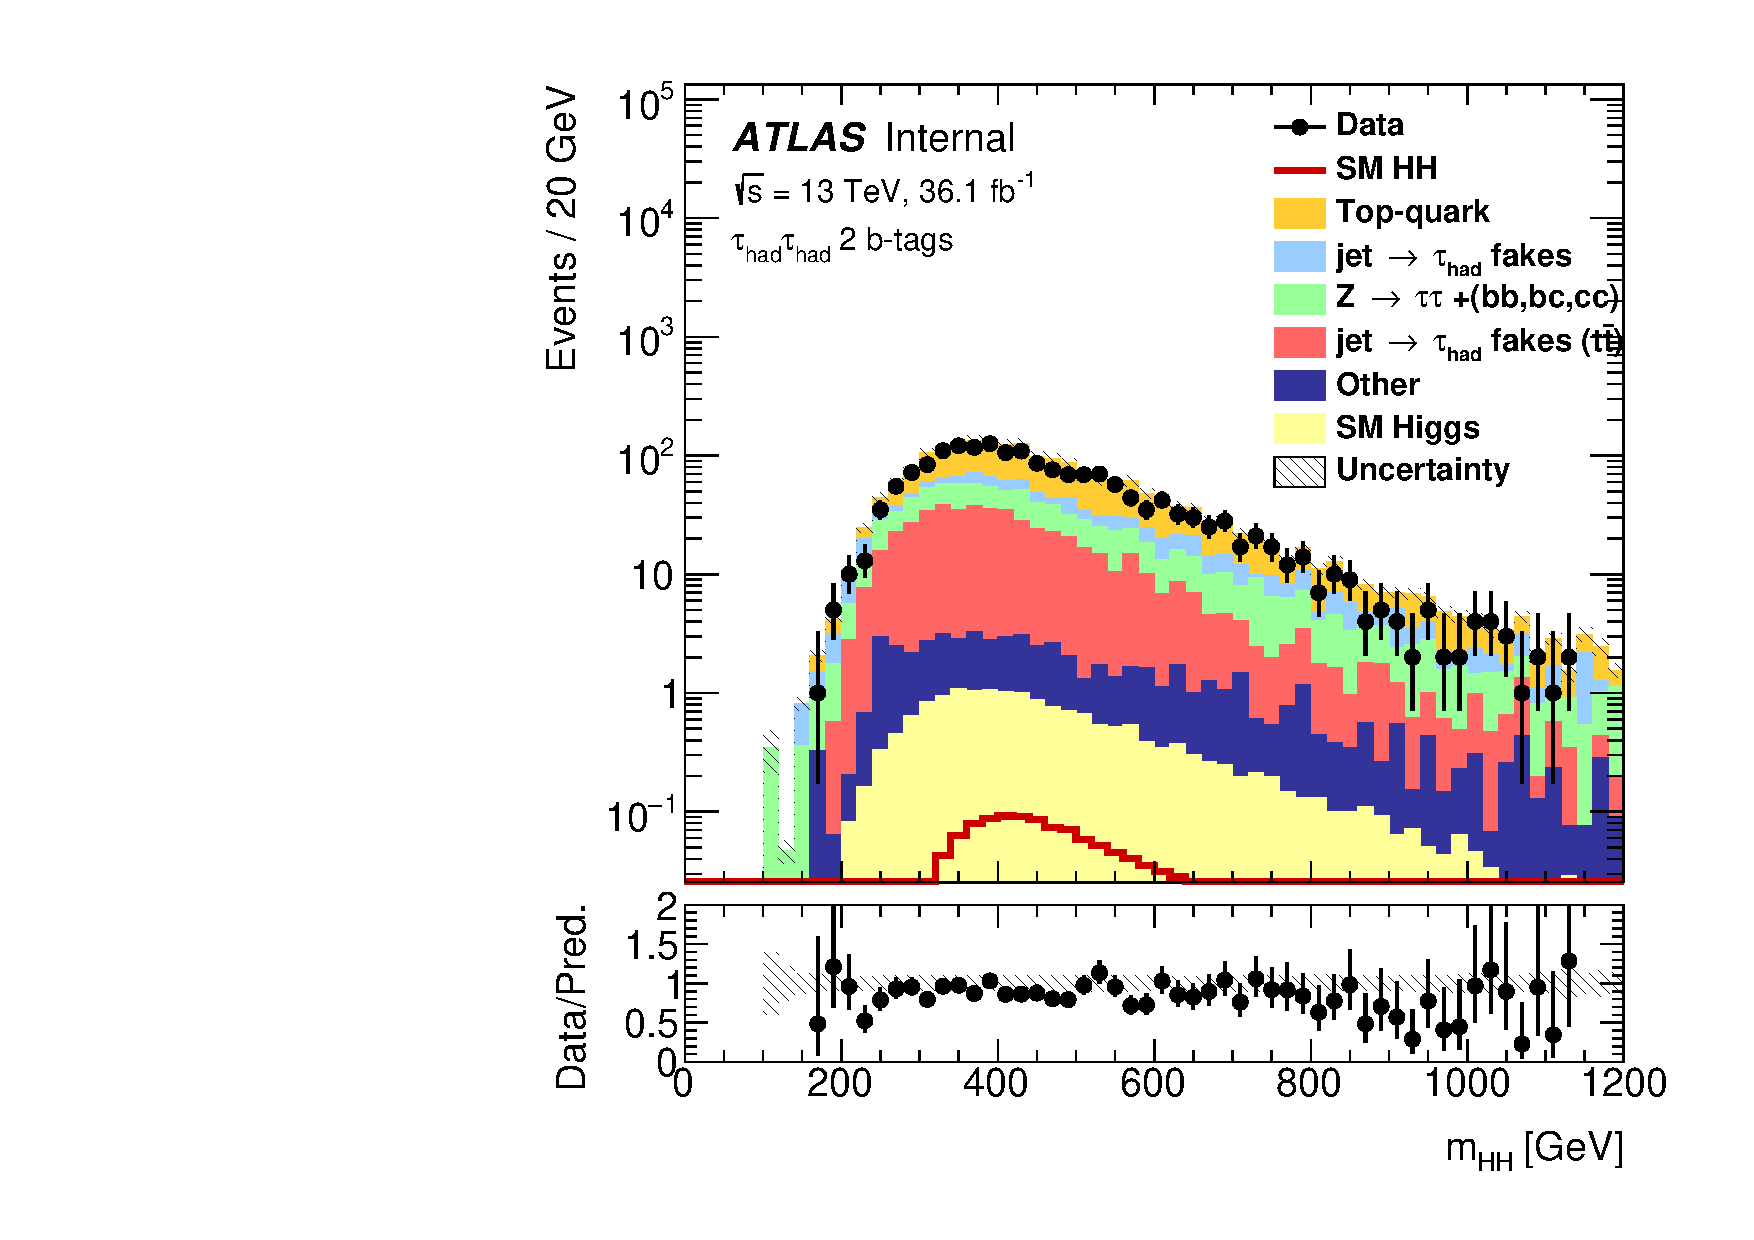
\includegraphics[width=.45\textwidth]{figures/selection/HadHad_HH/Plots2015/Region_BMin0_incJet1_distmHH_J2_Y2015_DLLOS_T2_SpcTauHH_L0_Prefitlog.pdf}
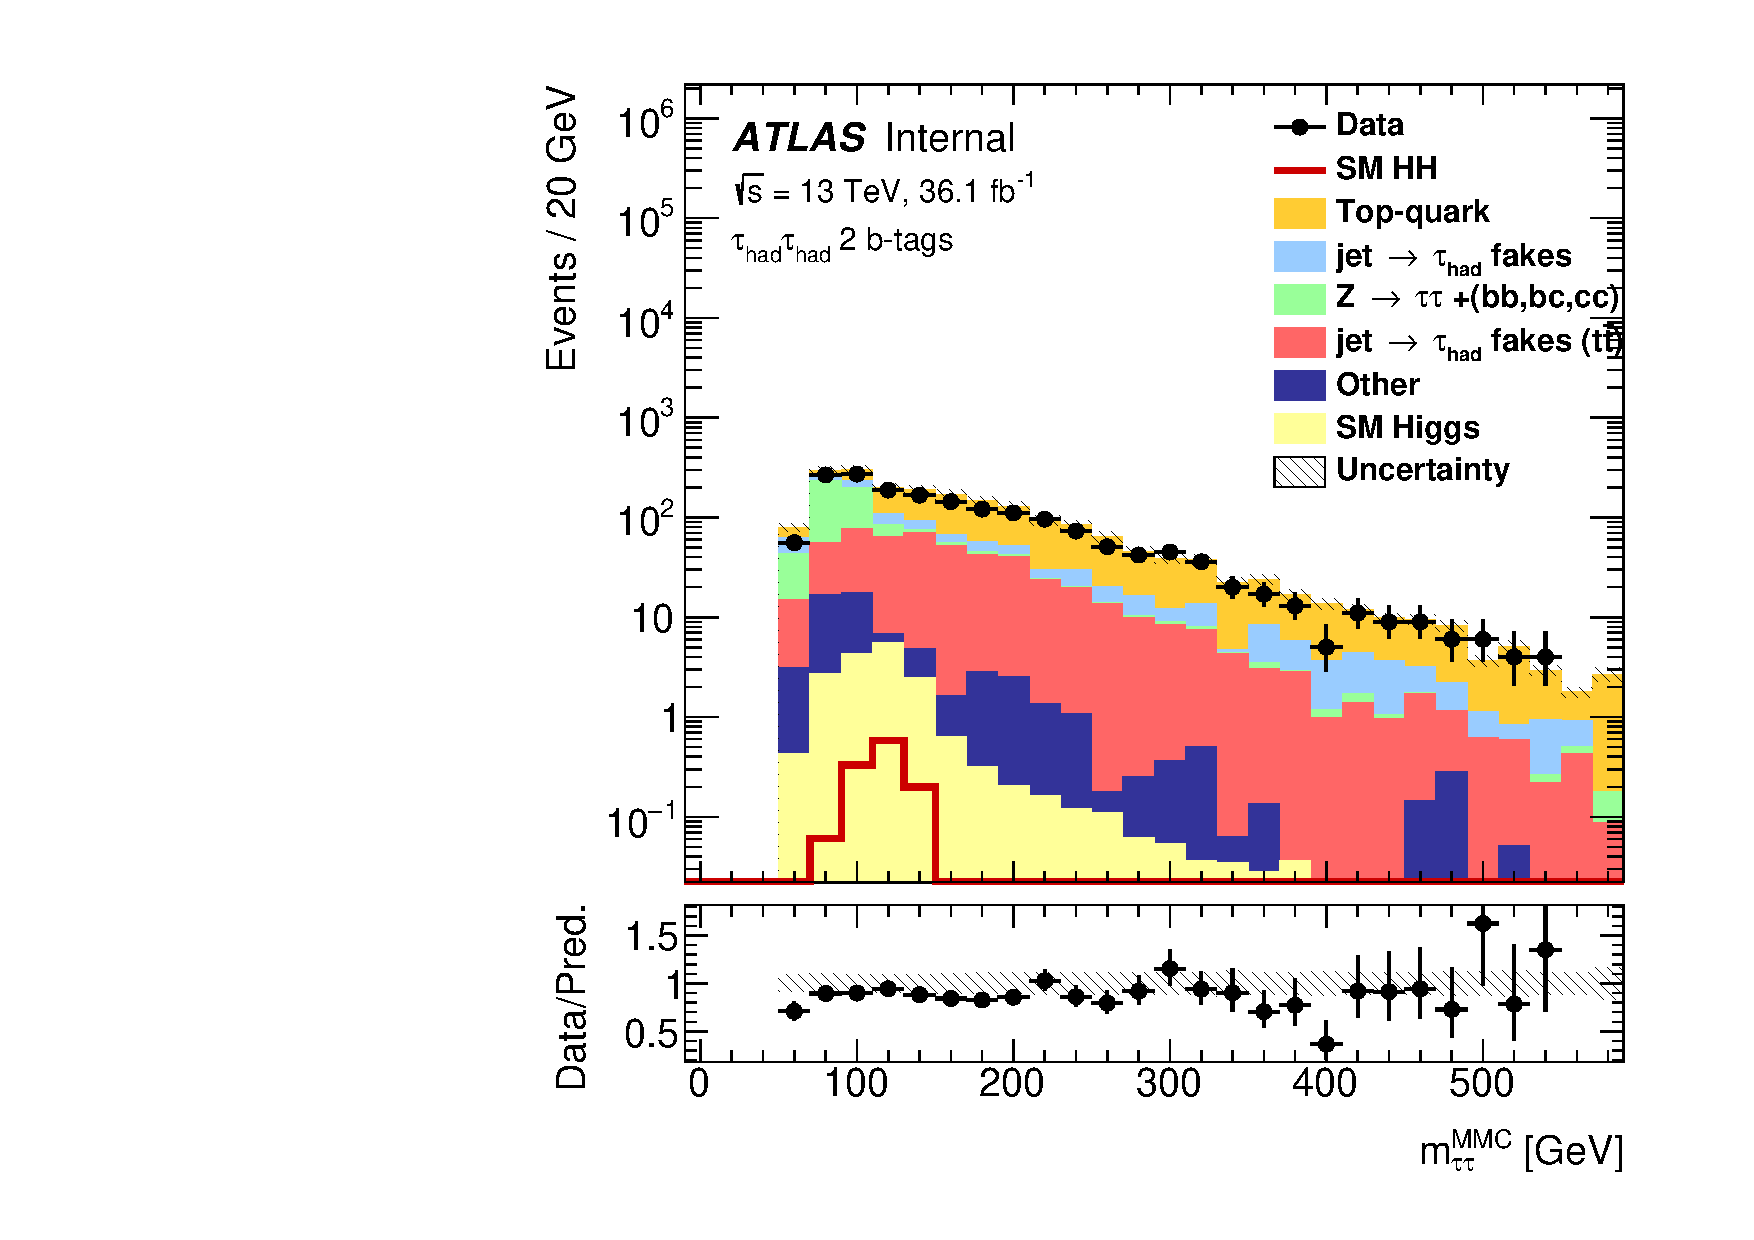
\includegraphics[width=.45\textwidth]{figures/selection/HadHad_HH/Plots2015/Region_BMin0_incJet1_distmMMC_J2_Y2015_DLLOS_T2_SpcTauHH_L0_Prefitlog.pdf}\\
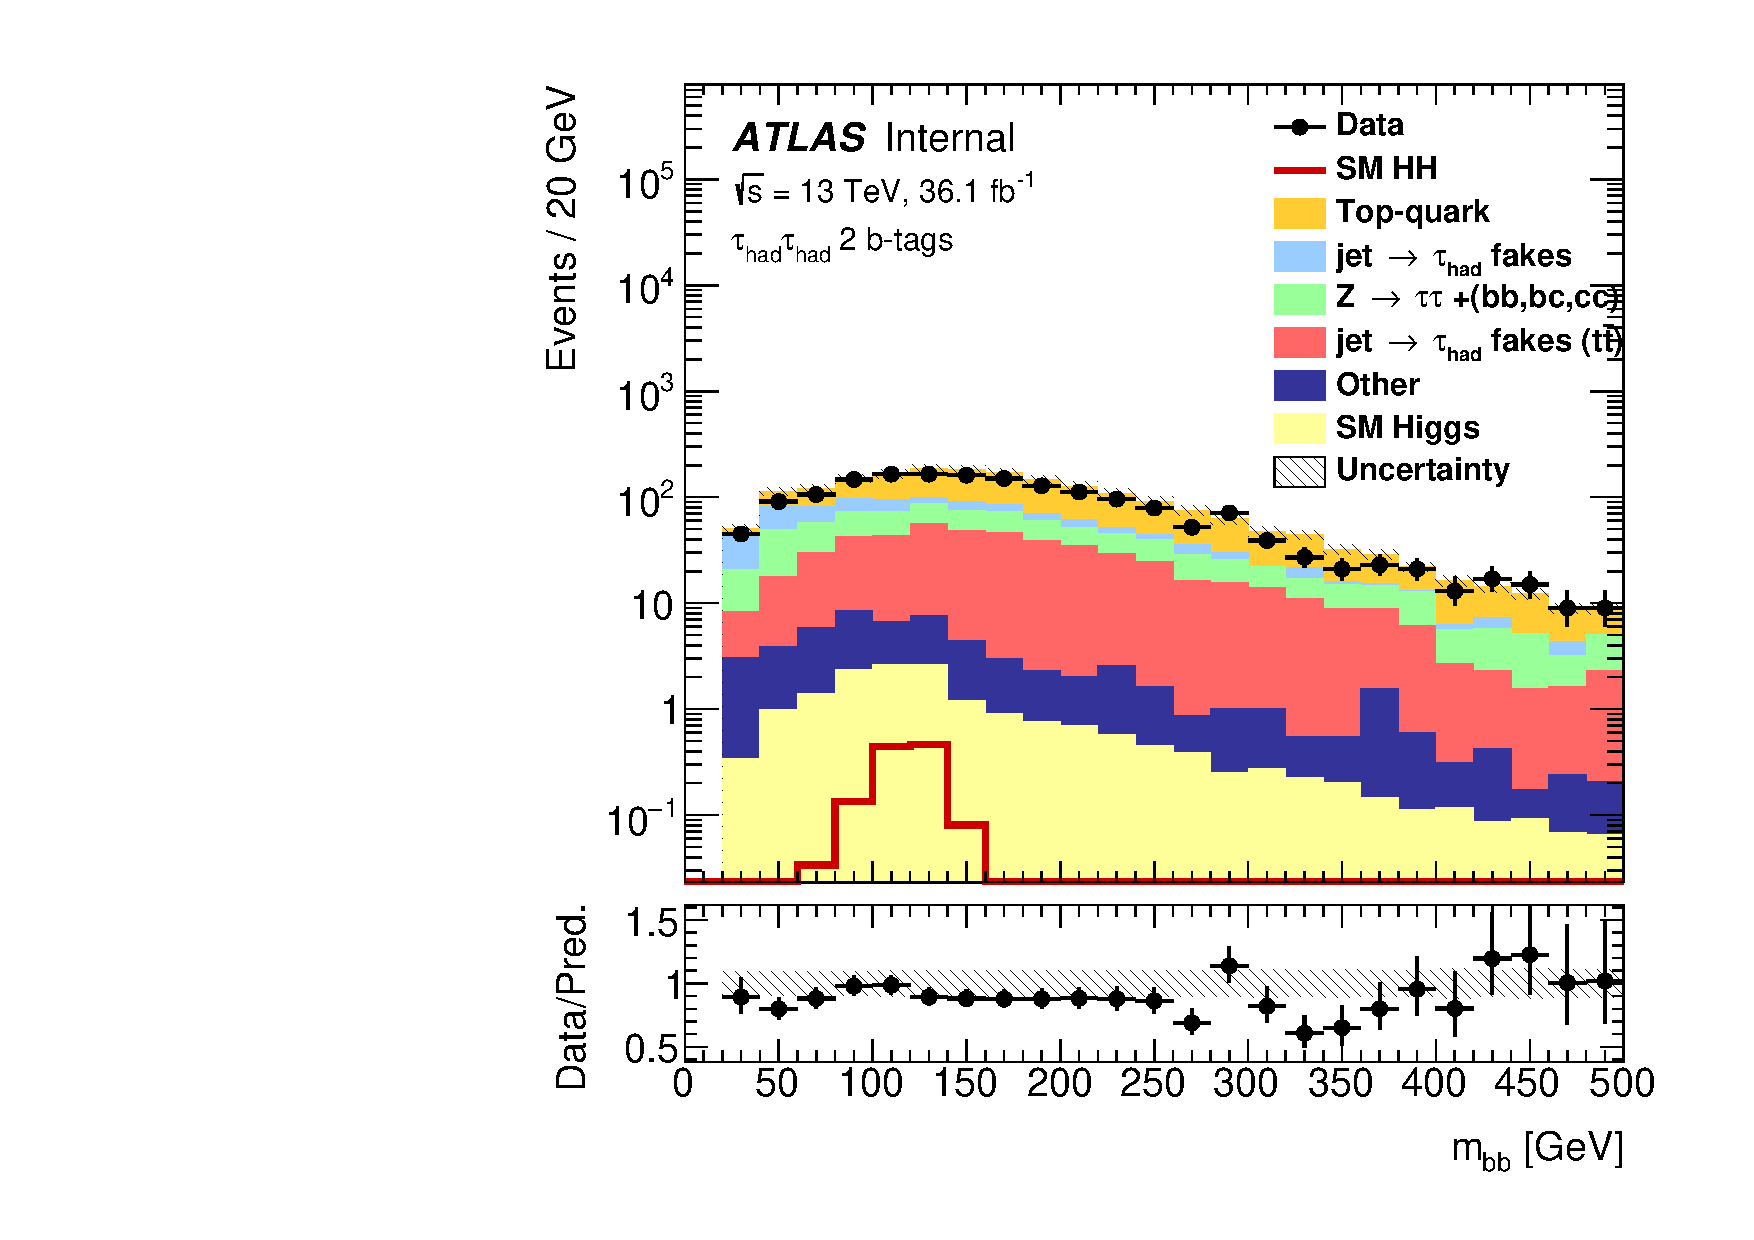
\includegraphics[width=.45\textwidth]{figures/selection/HadHad_HH/Plots2015/Region_BMin0_incJet1_distmBB_J2_Y2015_DLLOS_T2_SpcTauHH_L0_Prefitlog.pdf}
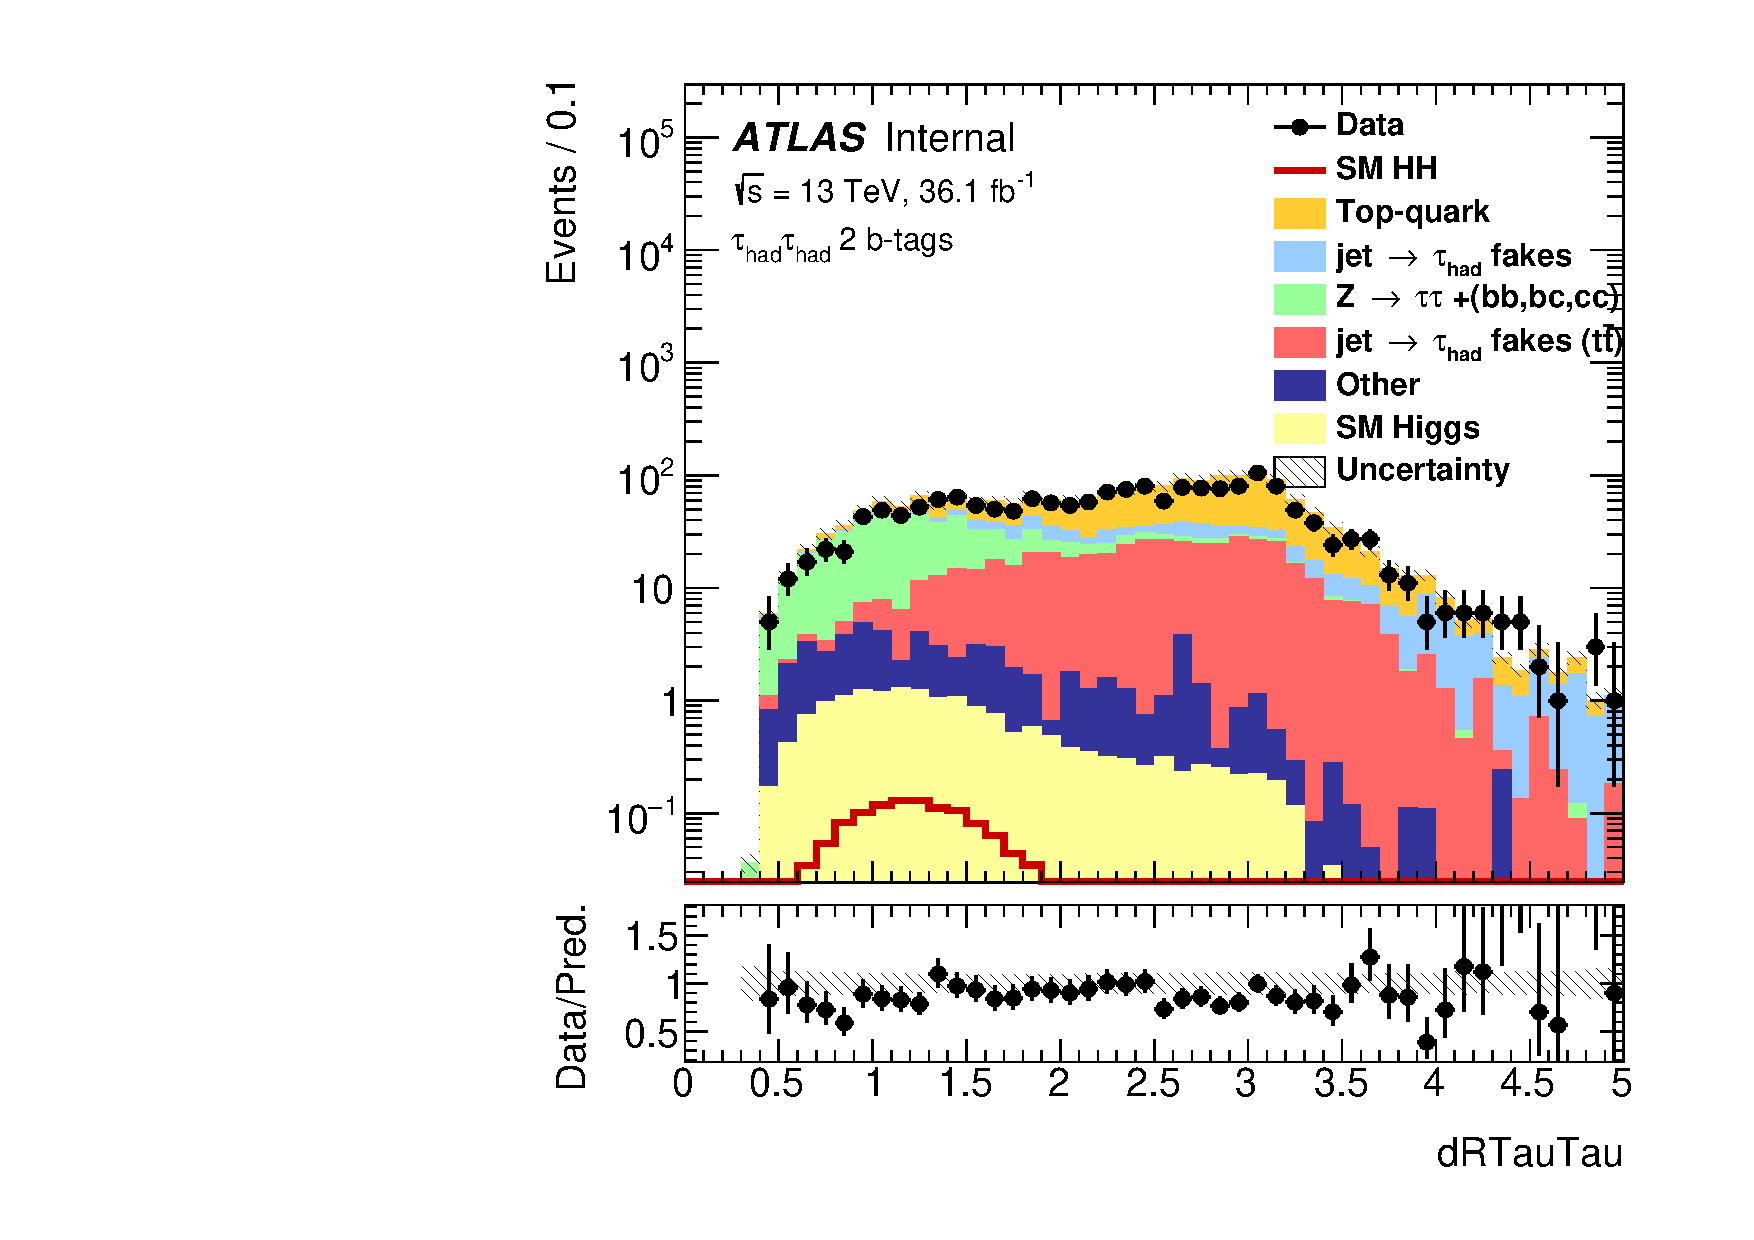
\includegraphics[width=.45\textwidth]{figures/selection/HadHad_HH/Plots2015/Region_BMin0_incJet1_distdRTauTau_J2_Y2015_DLLOS_T2_SpcTauHH_L0_Prefitlog.pdf}\\
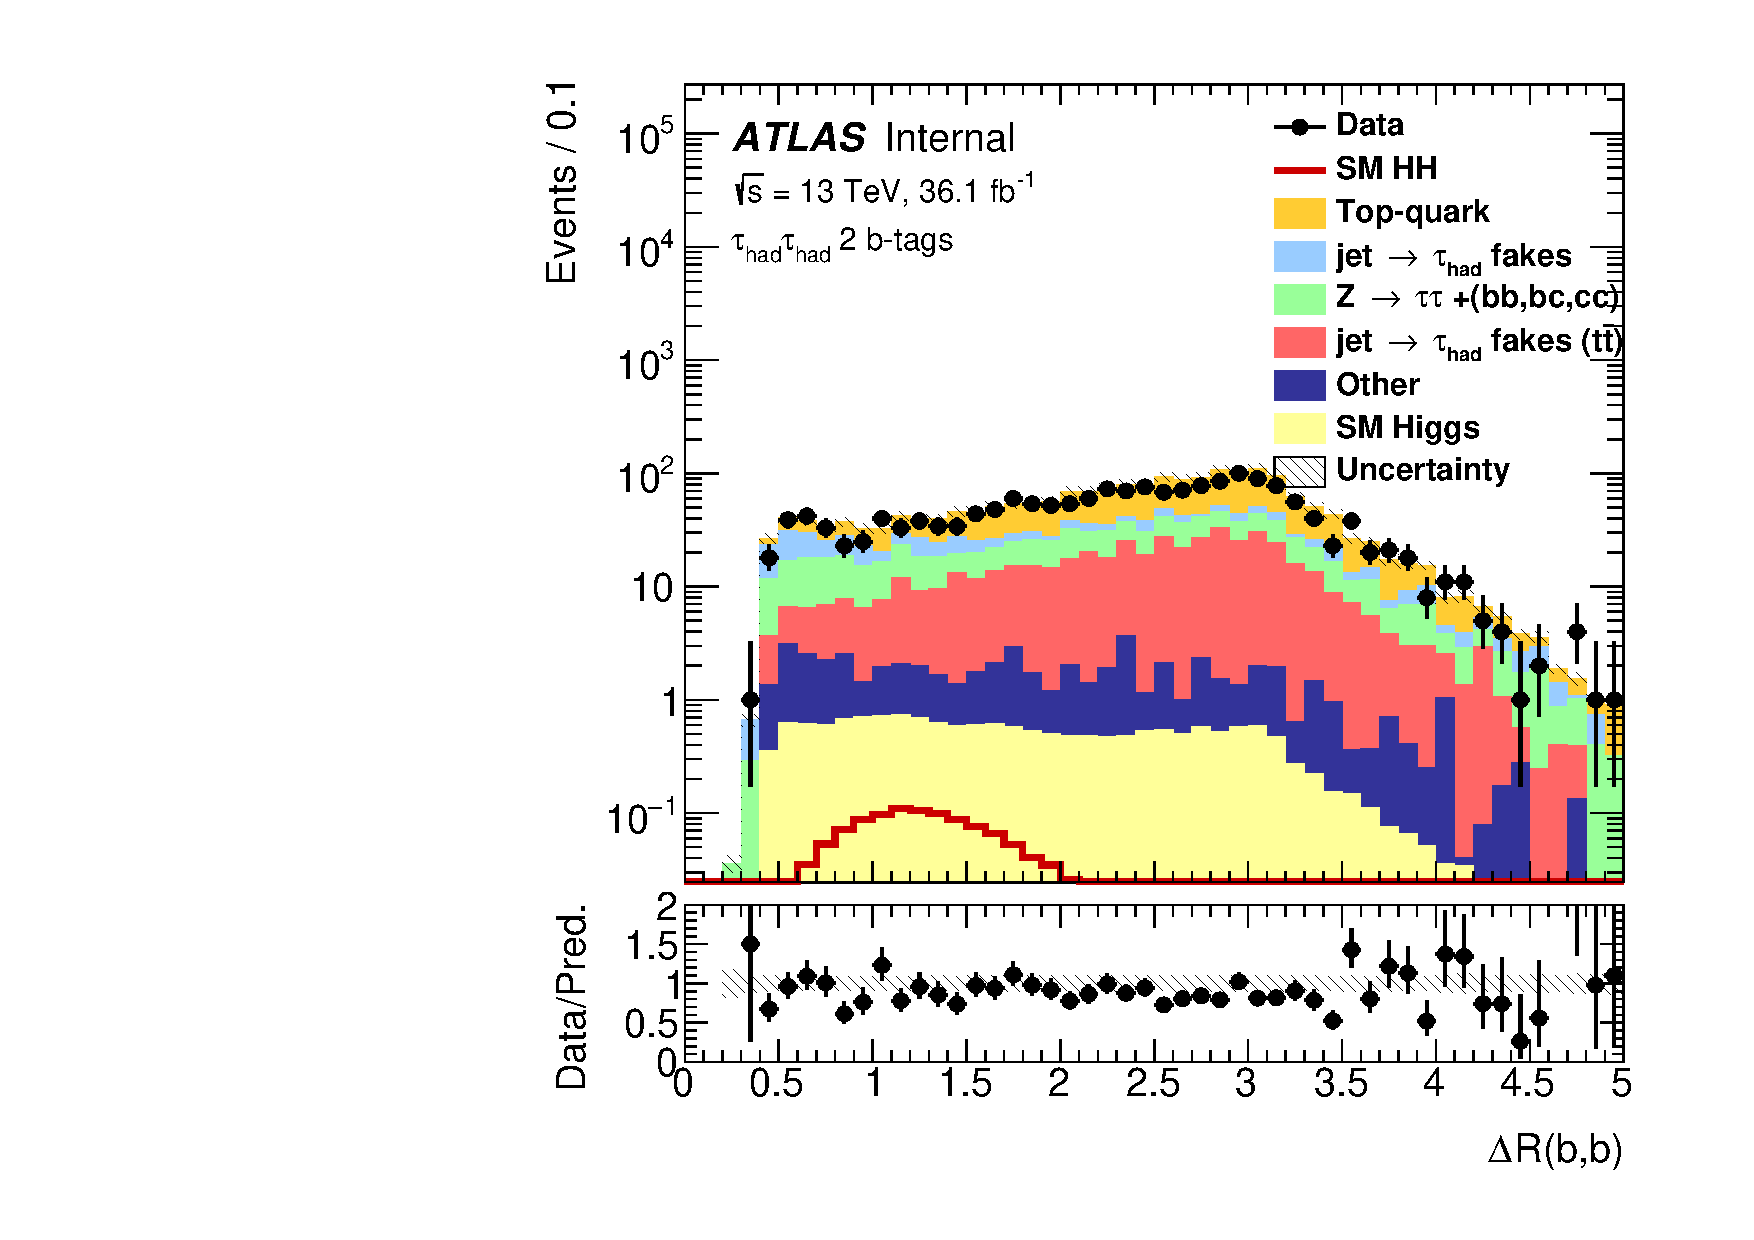
\includegraphics[width=.45\textwidth]{figures/selection/HadHad_HH/Plots2015/Region_BMin0_incJet1_distdRBB_J2_Y2015_DLLOS_T2_SpcTauHH_L0_Prefitlog.pdf}
\caption{Pre-fit MVA input variable distributions in the di-Higgs
  $bb\tau_{had}\tau_{had}$ signal region for the 2015-2016 data-taking period. The uncertainty band includes all uncertainties. The signal is normalised to the input cross section. (Inputs from 2021\_01\_15).}
\label{fig:HadHadPreselectionPNNInputsDistributions2015}
\end{figure}

\begin{figure}
\centering
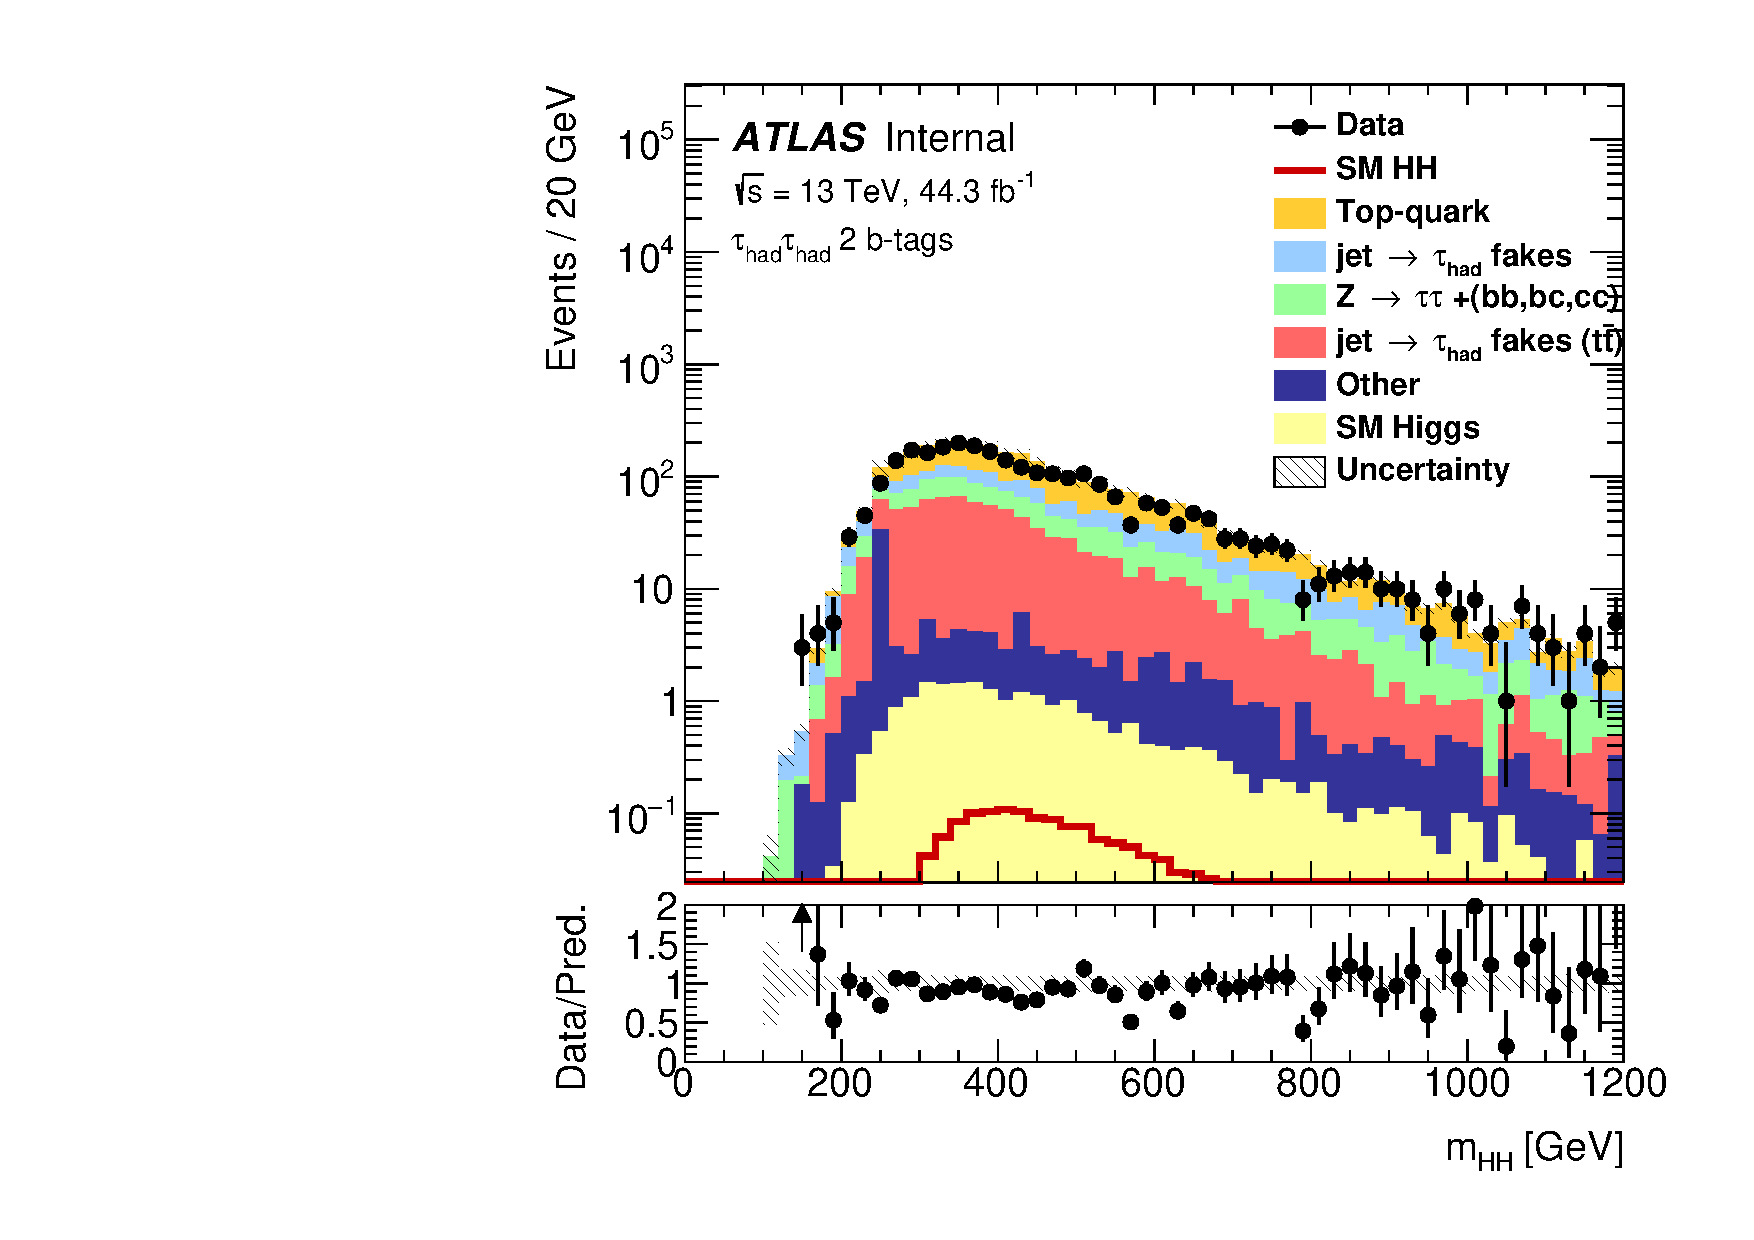
\includegraphics[width=.45\textwidth]{figures/selection/HadHad_HH/Plots2017/Region_BMin0_incJet1_distmHH_J2_Y2015_DLLOS_T2_SpcTauHH_L0_Prefitlog.pdf}
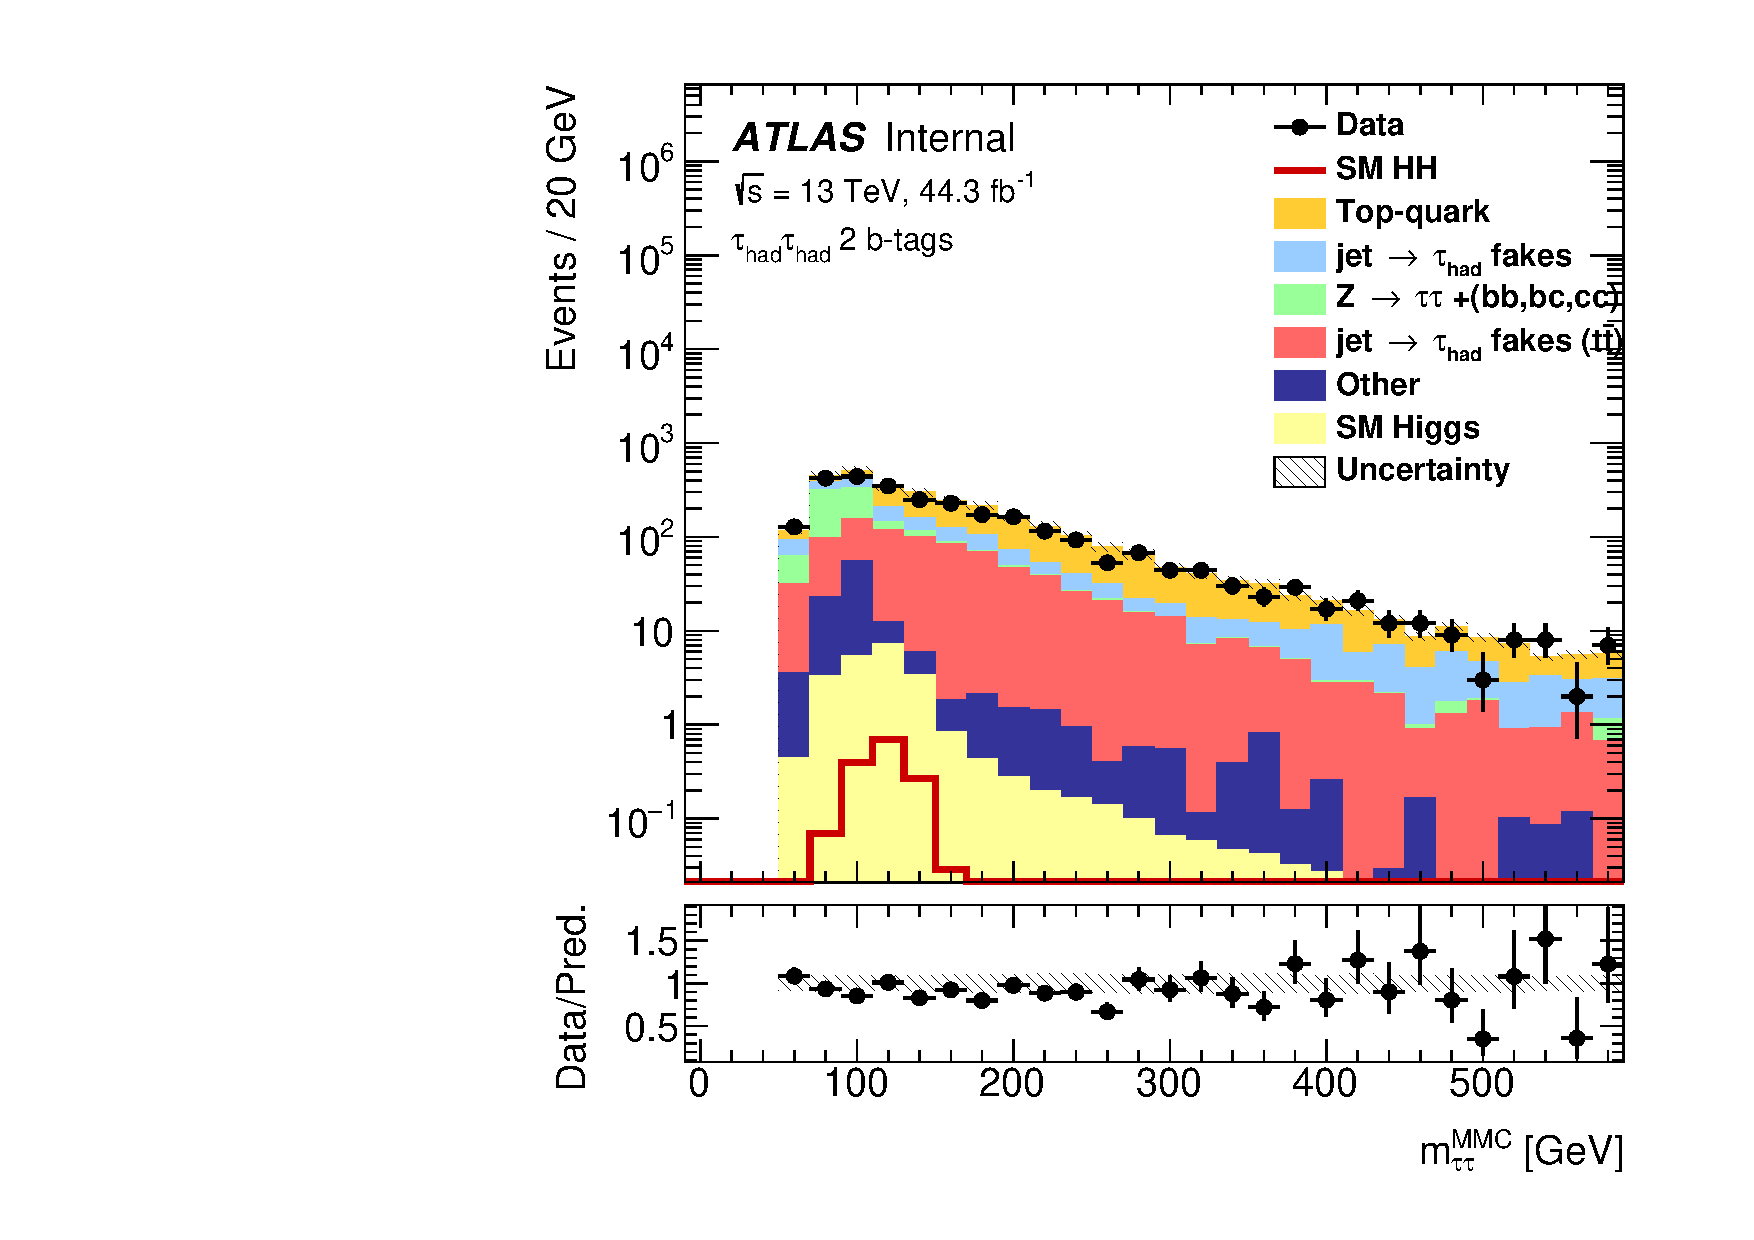
\includegraphics[width=.45\textwidth]{figures/selection/HadHad_HH/Plots2017/Region_BMin0_incJet1_distmMMC_J2_Y2015_DLLOS_T2_SpcTauHH_L0_Prefitlog.pdf}\\
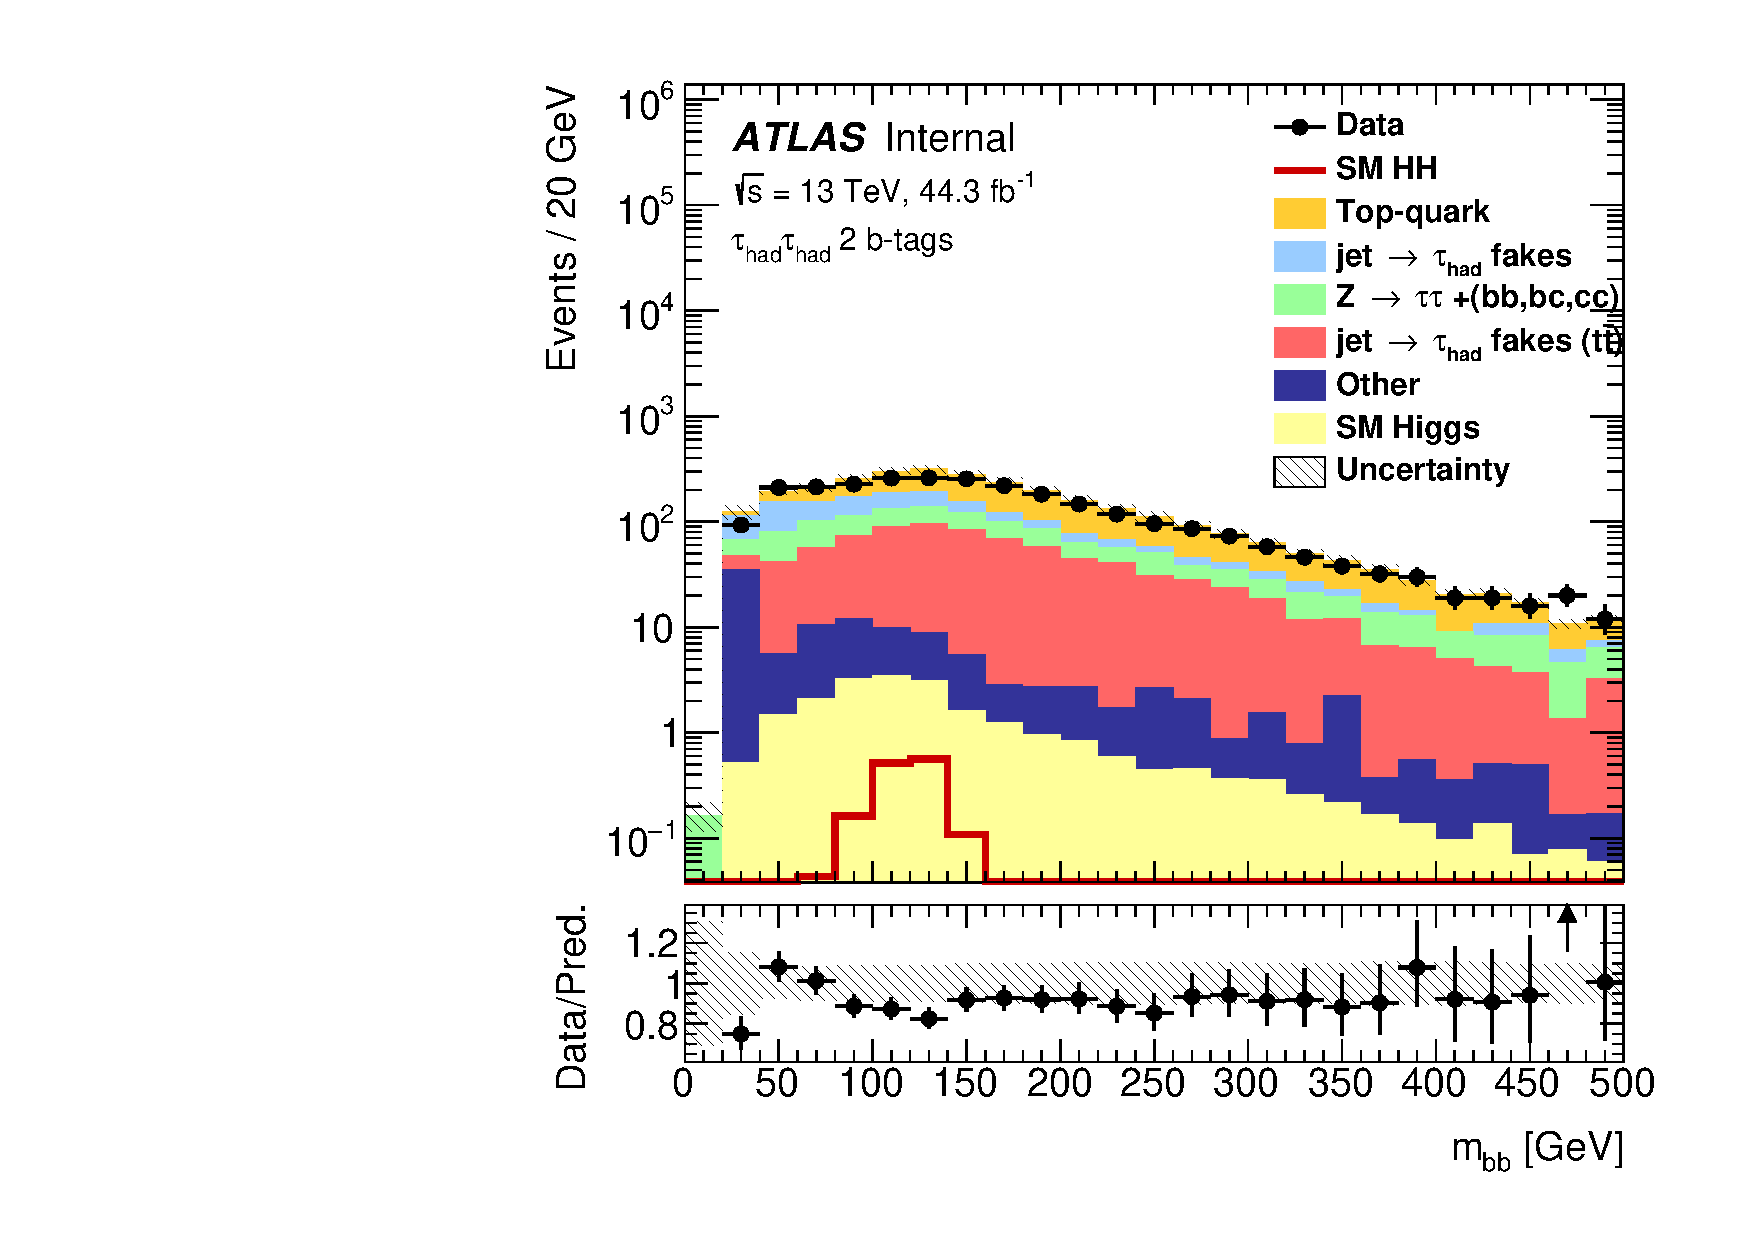
\includegraphics[width=.45\textwidth]{figures/selection/HadHad_HH/Plots2017/Region_BMin0_incJet1_distmBB_J2_Y2015_DLLOS_T2_SpcTauHH_L0_Prefitlog.pdf}
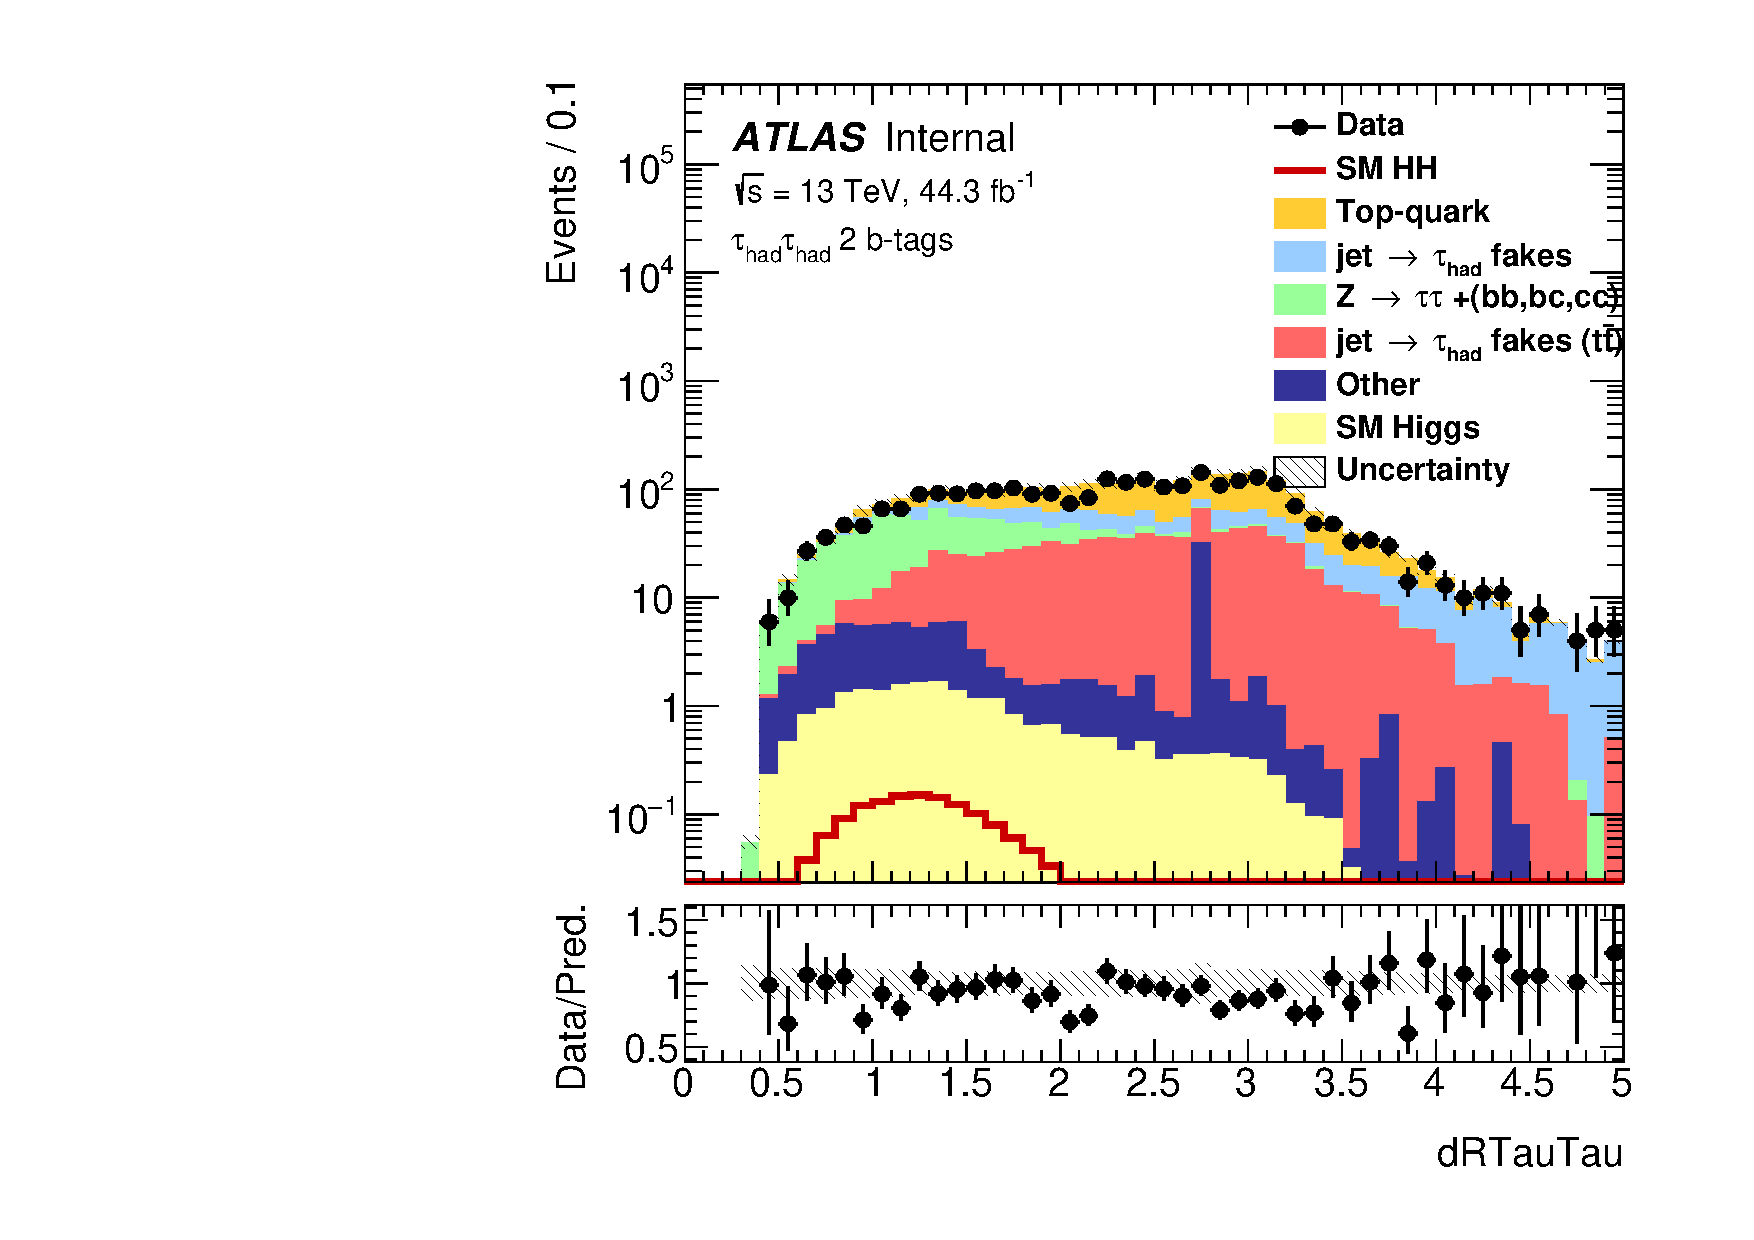
\includegraphics[width=.45\textwidth]{figures/selection/HadHad_HH/Plots2017/Region_BMin0_incJet1_distdRTauTau_J2_Y2015_DLLOS_T2_SpcTauHH_L0_Prefitlog.pdf}\\
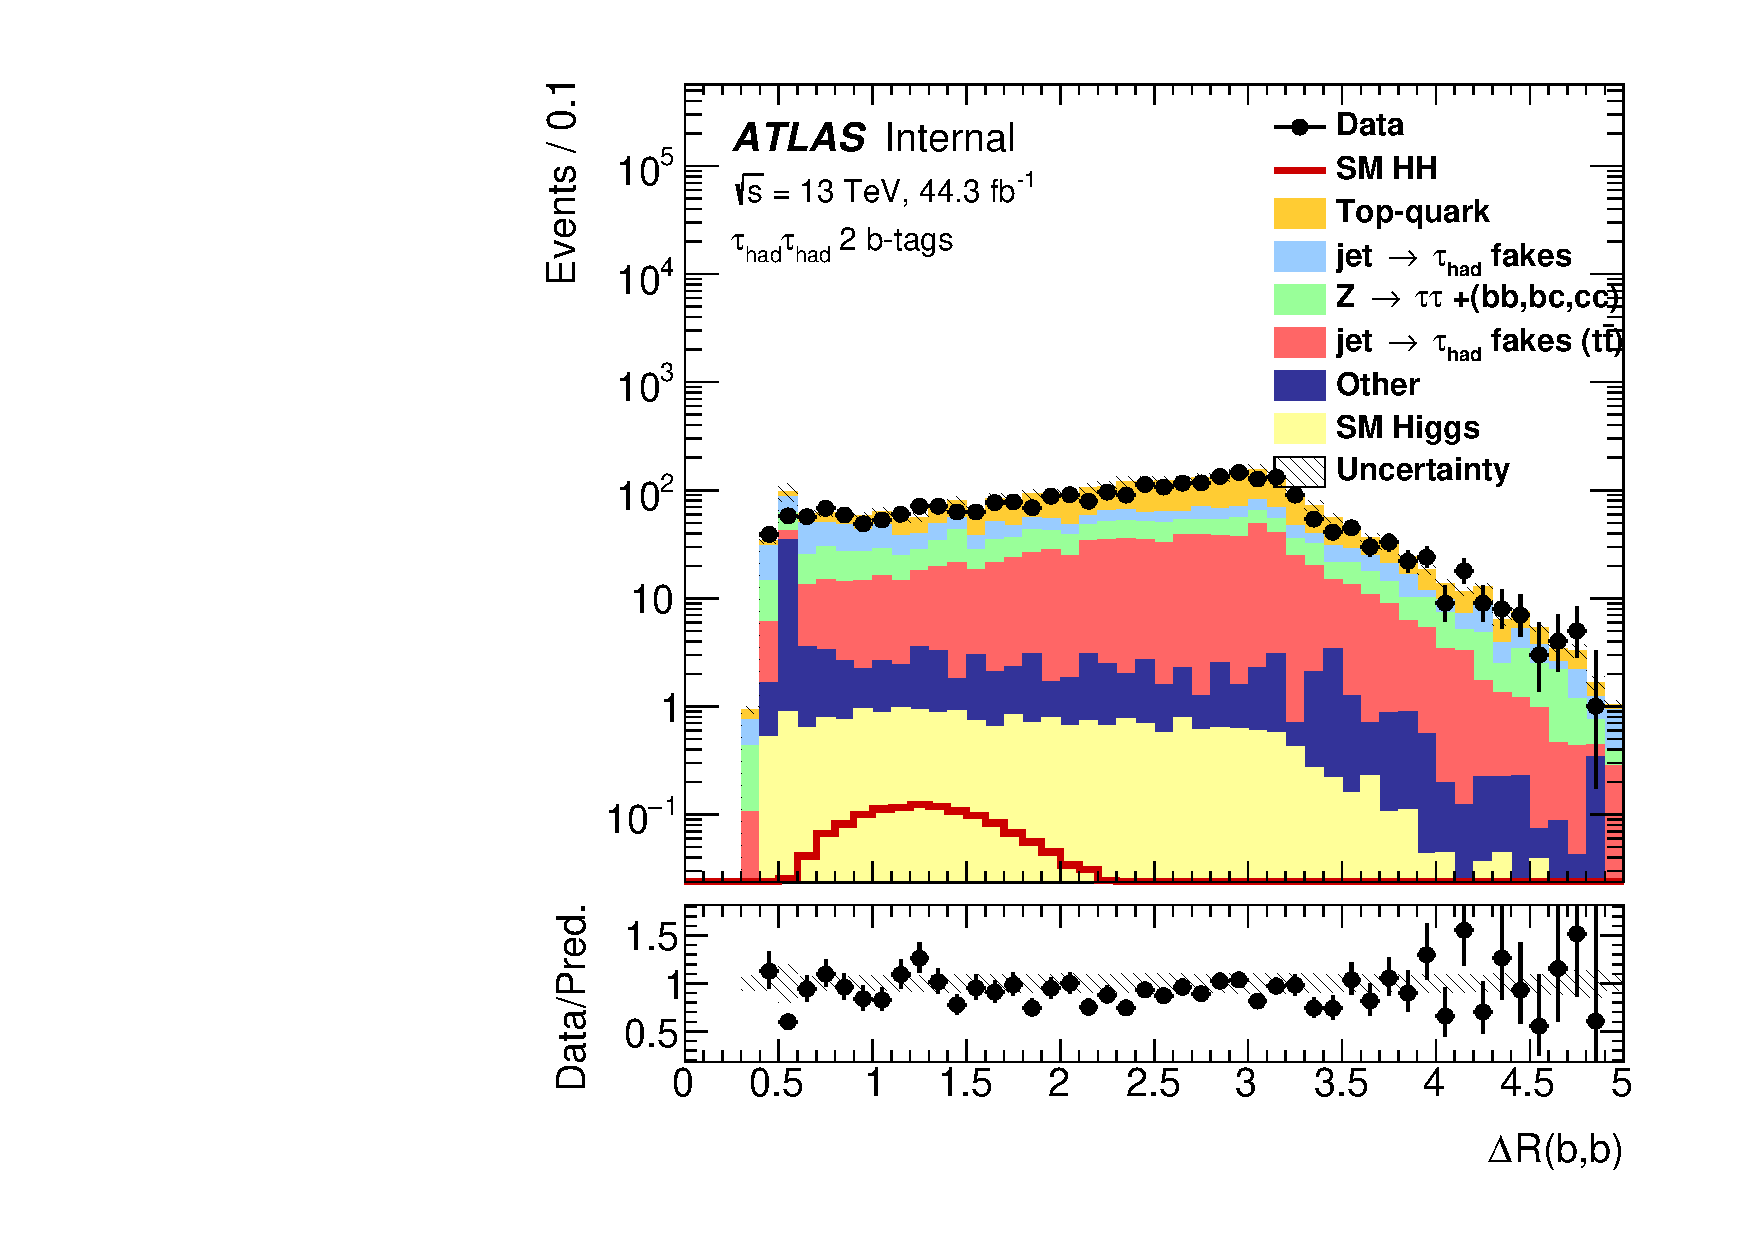
\includegraphics[width=.45\textwidth]{figures/selection/HadHad_HH/Plots2017/Region_BMin0_incJet1_distdRBB_J2_Y2015_DLLOS_T2_SpcTauHH_L0_Prefitlog.pdf}
\caption{Pre-fit MVA input variable distributions in the di-Higgs
  $bb\tau_{had}\tau_{had}$ signal region for the 2017 data-taking period. The uncertainty band includes all uncertainties. The signal is normalised to the input cross section. (Inputs from 2021\_01\_15).}
\label{fig:HadHadPreselectionPNNInputsDistributions2017}
\end{figure}


\begin{figure}
\centering
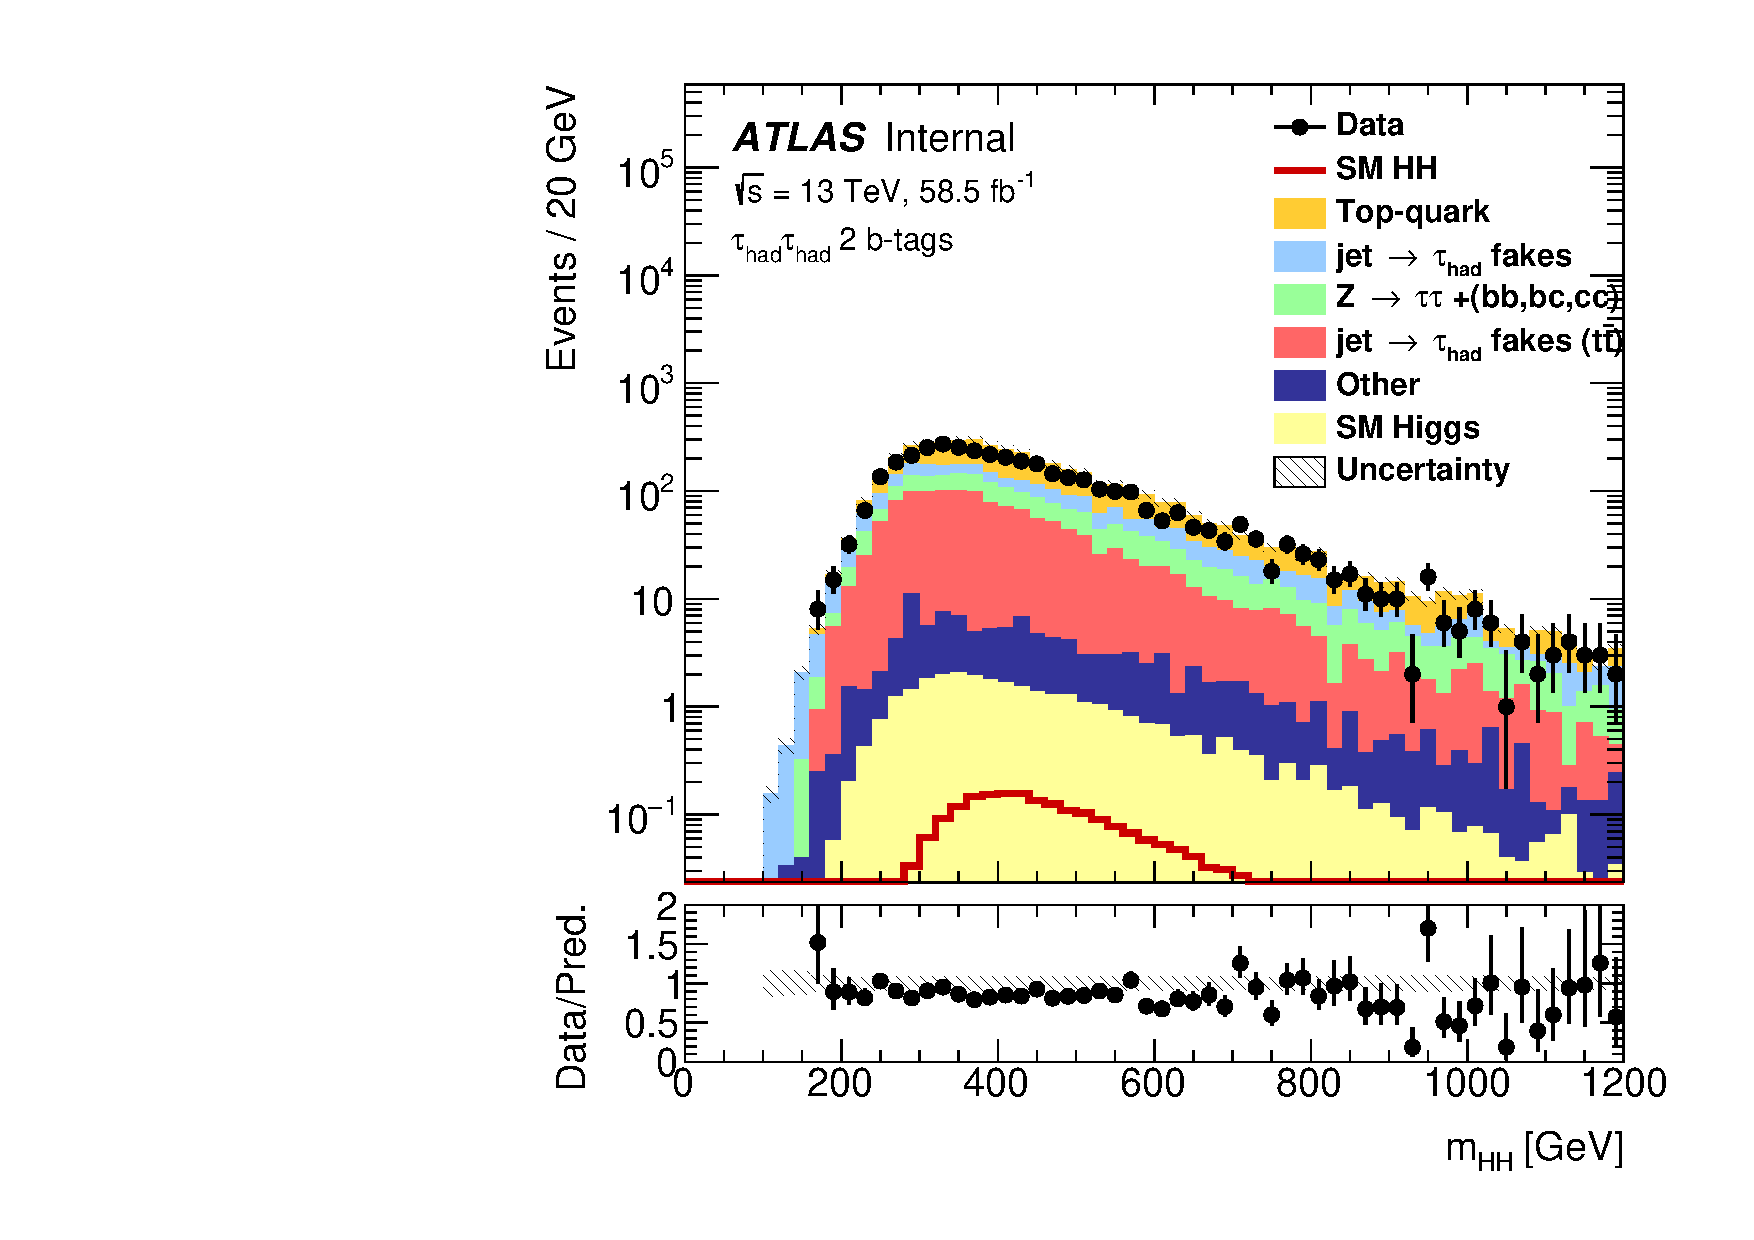
\includegraphics[width=.45\textwidth]{figures/selection/HadHad_HH/Plots2018/Region_BMin0_incJet1_distmHH_J2_Y2015_DLLOS_T2_SpcTauHH_L0_Prefitlog.pdf}
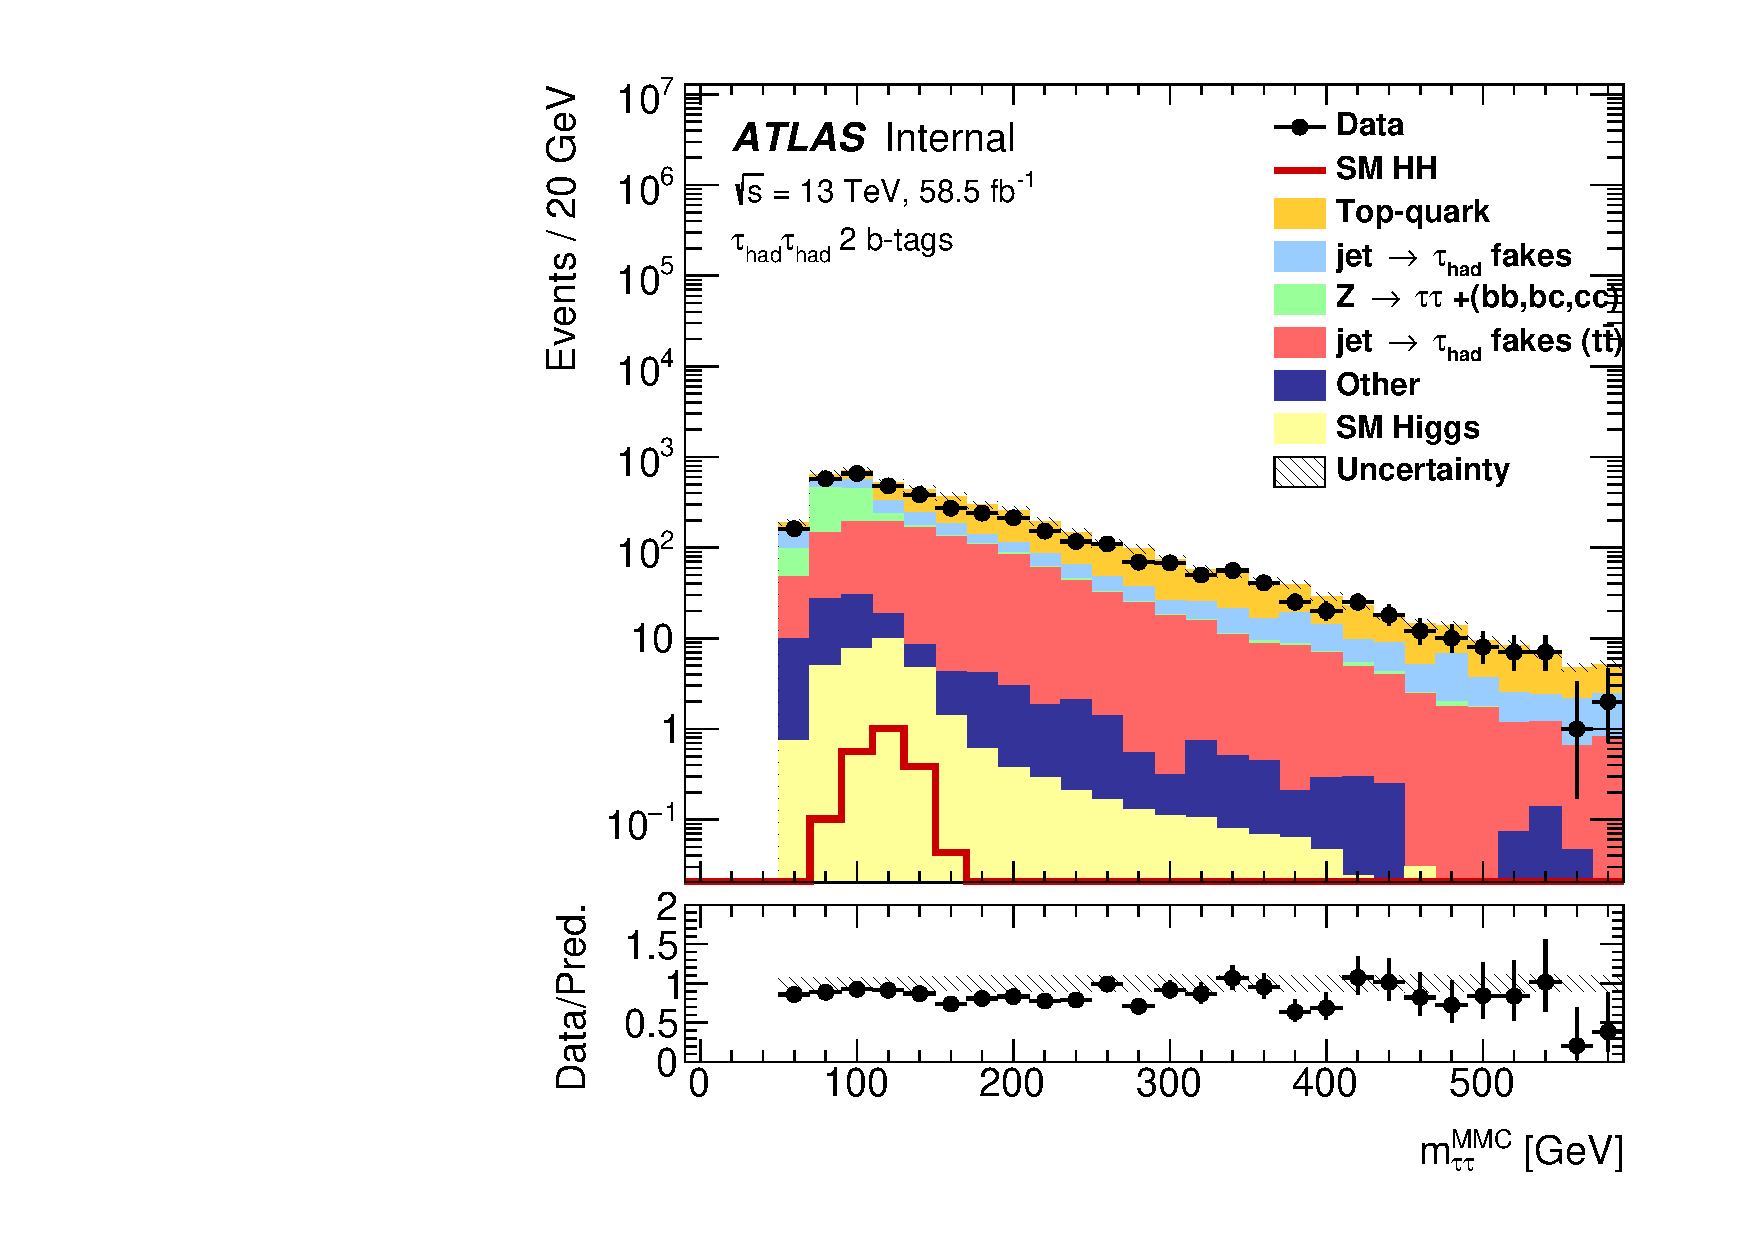
\includegraphics[width=.45\textwidth]{figures/selection/HadHad_HH/Plots2018/Region_BMin0_incJet1_distmMMC_J2_Y2015_DLLOS_T2_SpcTauHH_L0_Prefitlog.pdf}\\
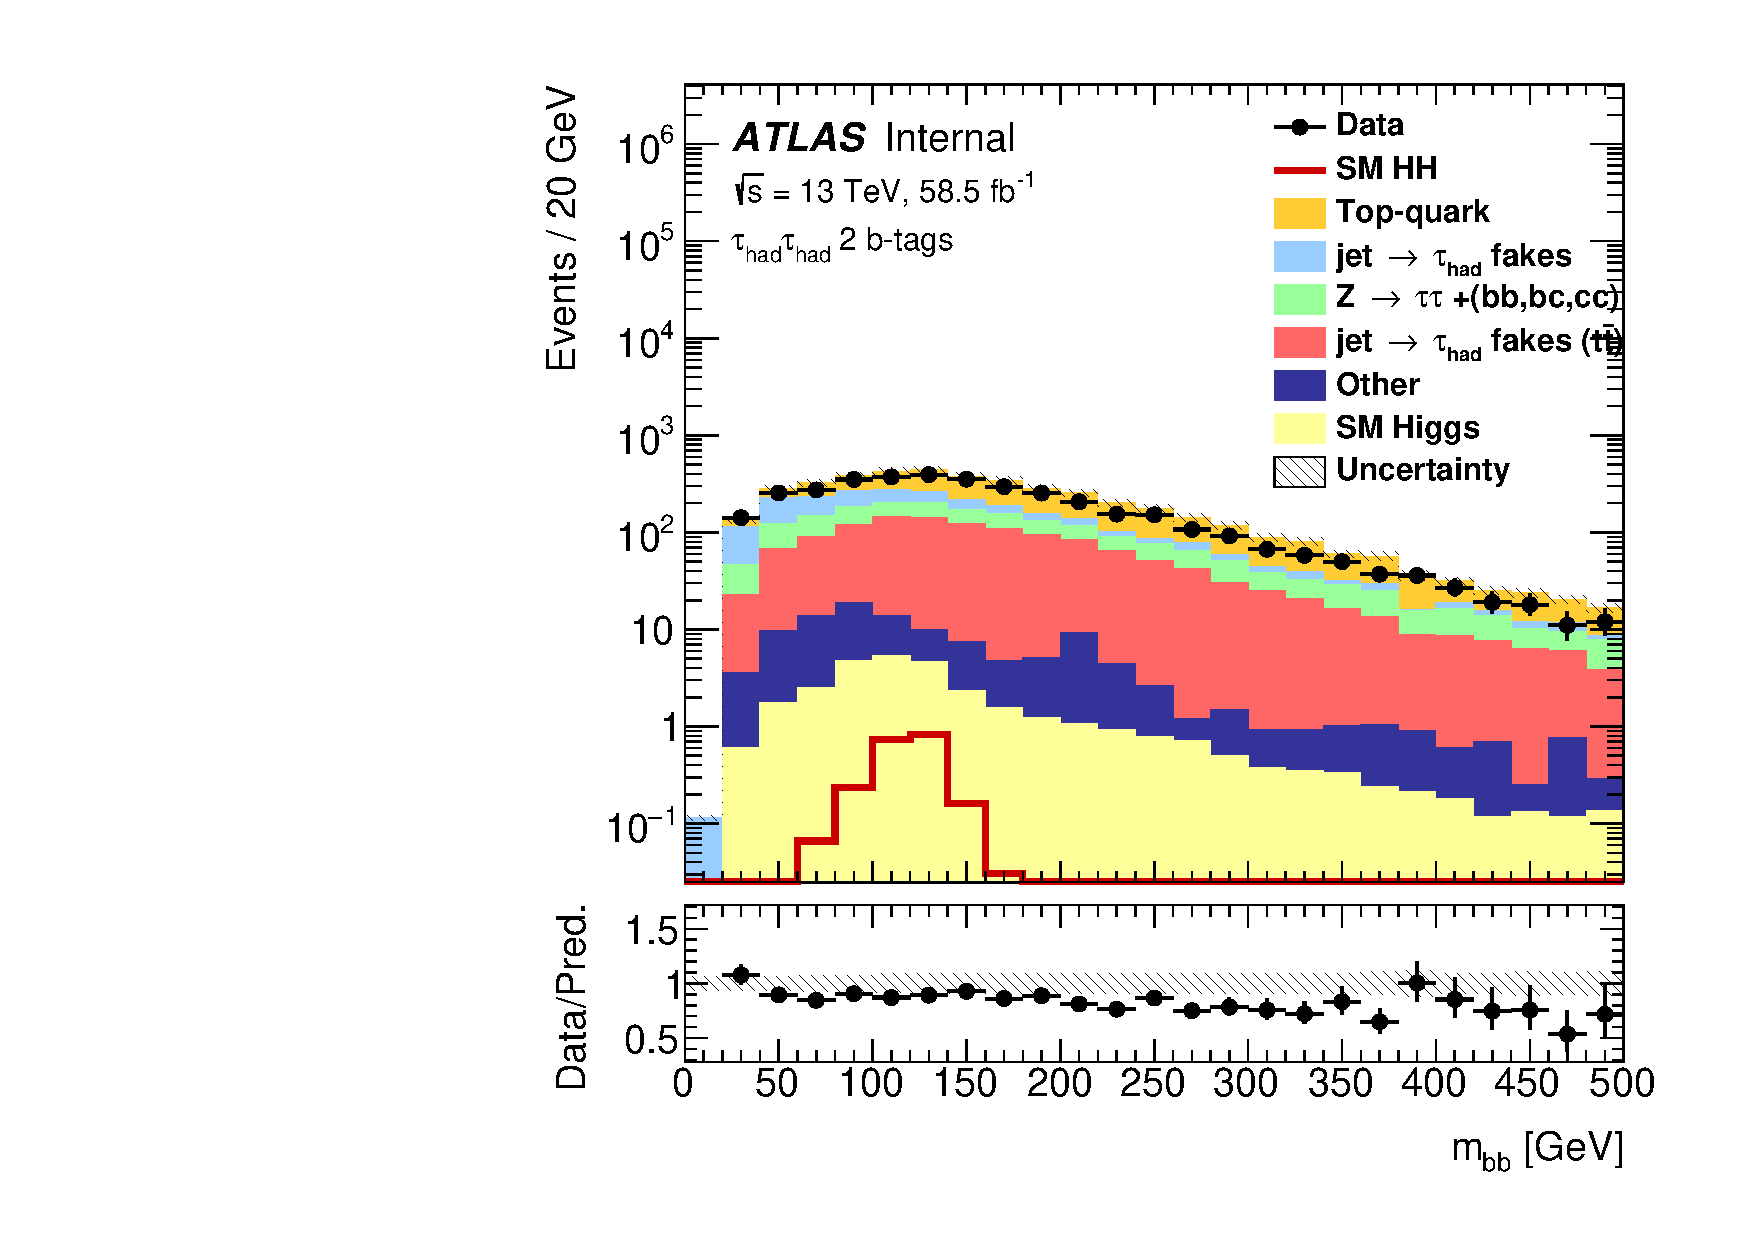
\includegraphics[width=.45\textwidth]{figures/selection/HadHad_HH/Plots2018/Region_BMin0_incJet1_distmBB_J2_Y2015_DLLOS_T2_SpcTauHH_L0_Prefitlog.pdf}
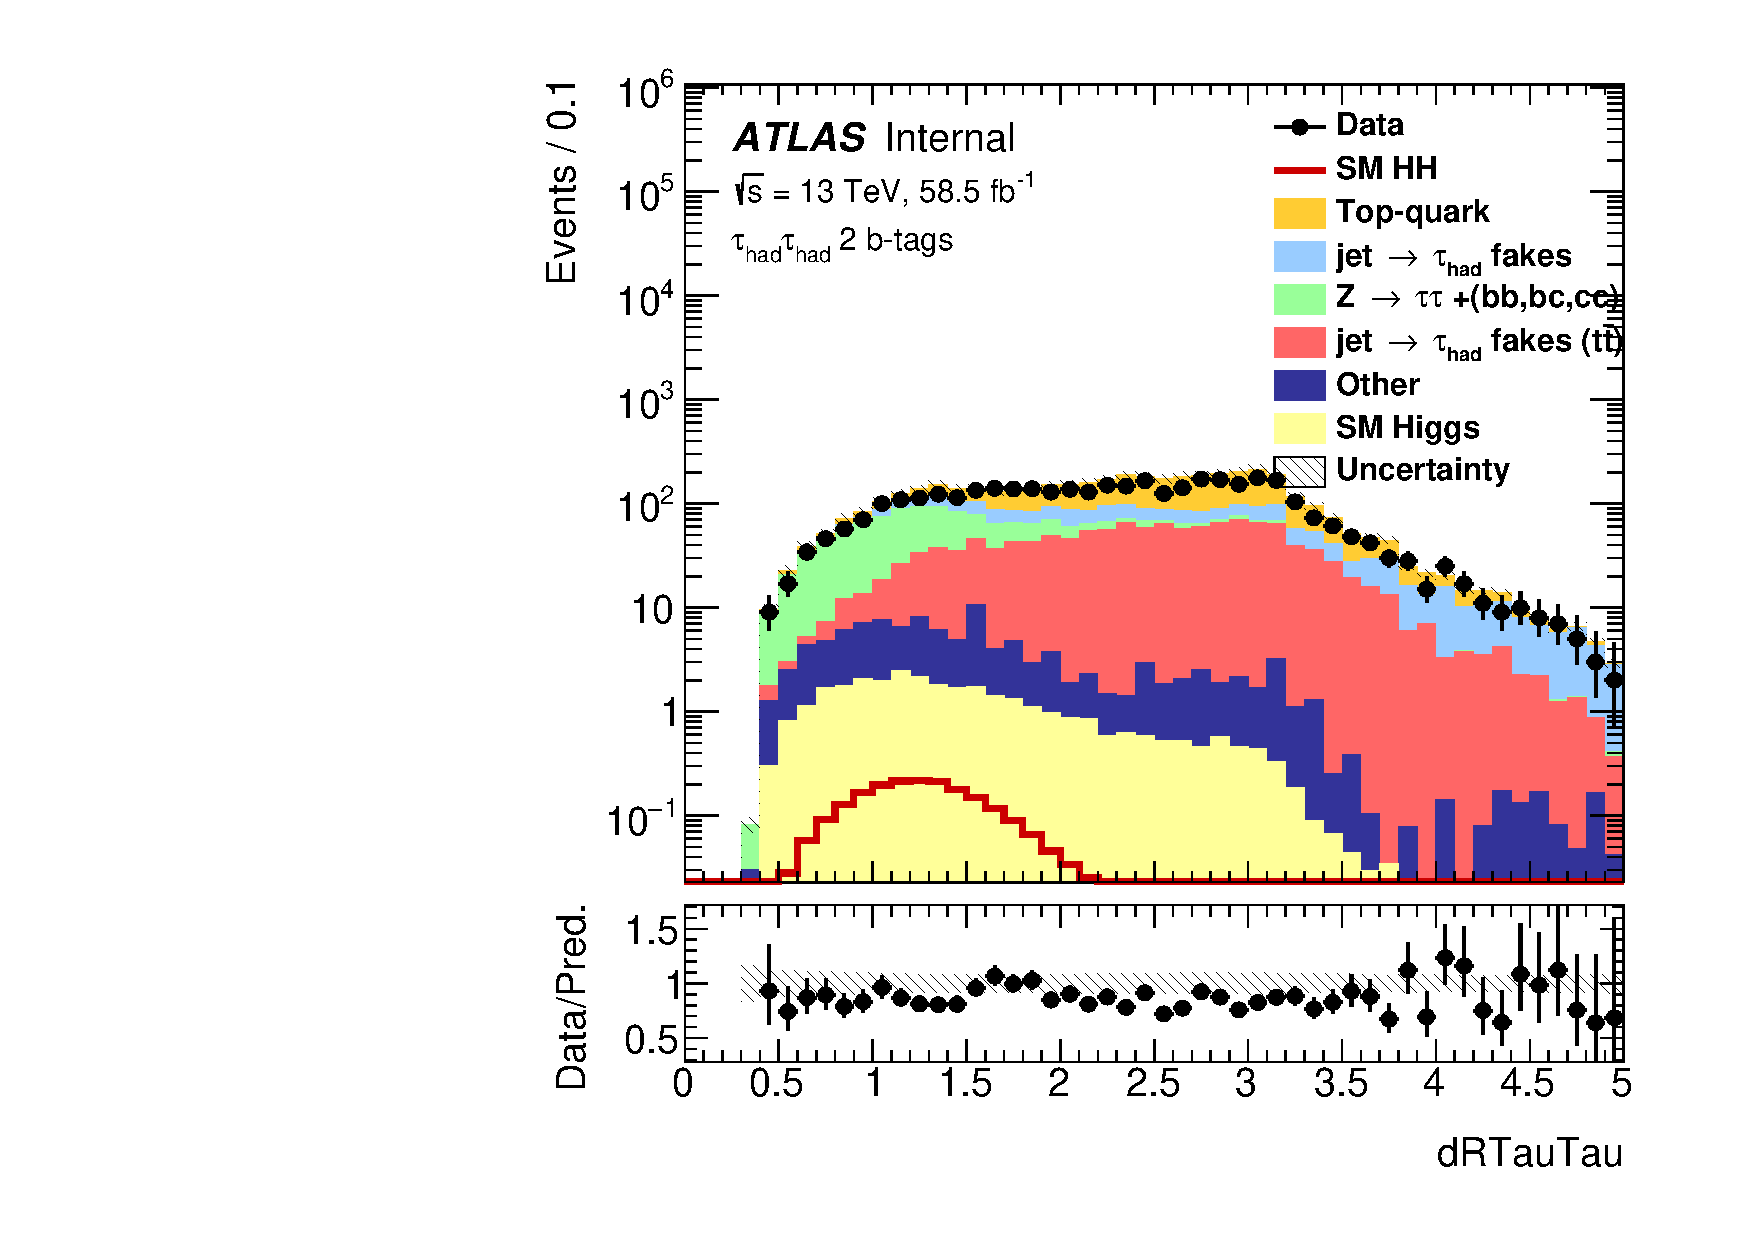
\includegraphics[width=.45\textwidth]{figures/selection/HadHad_HH/Plots2018/Region_BMin0_incJet1_distdRTauTau_J2_Y2015_DLLOS_T2_SpcTauHH_L0_Prefitlog.pdf}\\
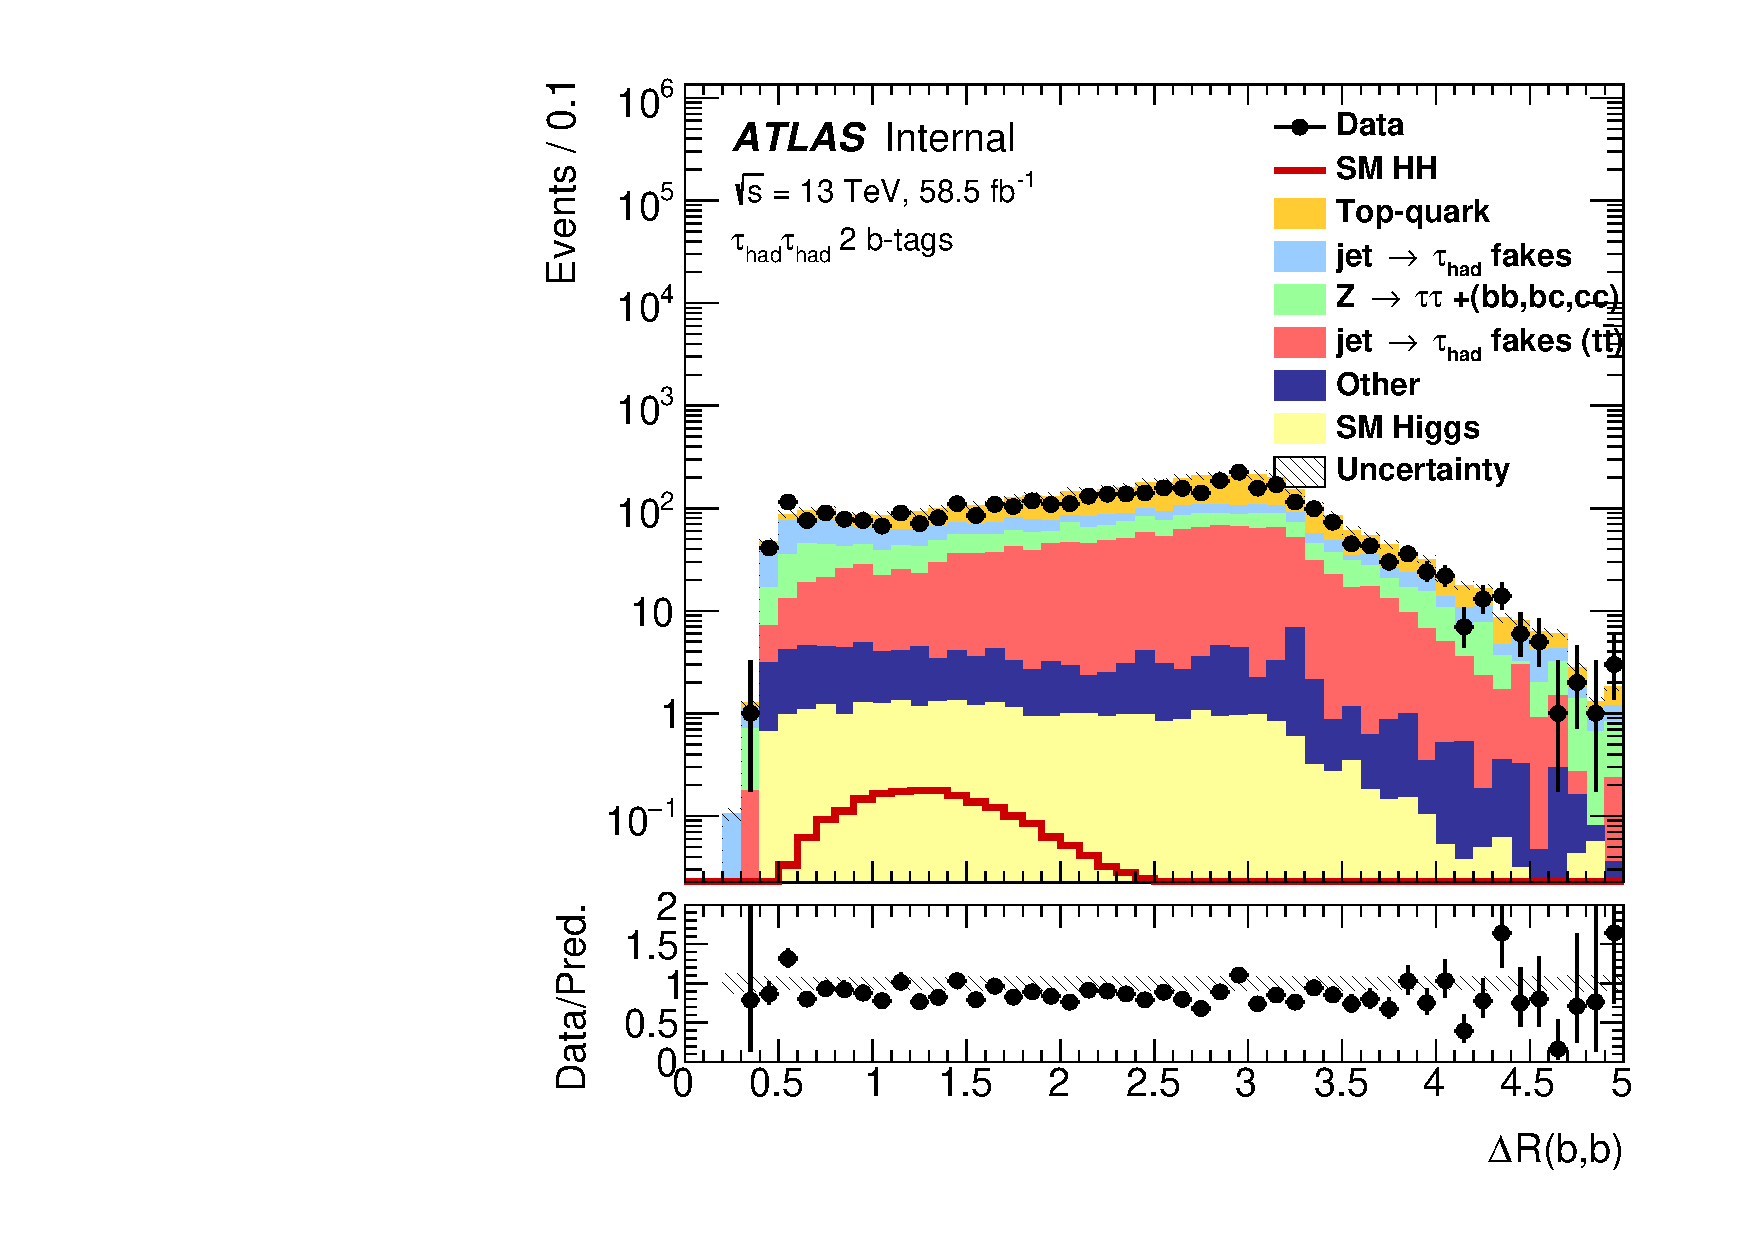
\includegraphics[width=.45\textwidth]{figures/selection/HadHad_HH/Plots2018/Region_BMin0_incJet1_distdRBB_J2_Y2015_DLLOS_T2_SpcTauHH_L0_Prefitlog.pdf}
\caption{Pre-fit MVA input variable distributions in the di-Higgs
  $bb\tau_{had}\tau_{had}$ signal region for the 2017 data-taking period. The uncertainty band includes all uncertainties. The signal is normalised to the input cross section. (Inputs from 2021\_01\_15).}
\label{fig:HadHadPreselectionPNNInputsDistributions2018}
\end{figure}



Figure~\ref{fig:HadHadPreselectionPNNScoreDistributions} shows the data/prediction comparison for the pre-fit PNN score distributions for the $300, 500, 1000, 1600$ GeV mass points and for the pre-fit SM BDT distribution in the $bb\tau_{had}\tau_{had}$ signal region.  The PNN score distributions for each mass point and the SM BDT distribution are used as final discriminants for the limit settings and are shown here with the binning used in the fit defined as described in Section~\ref{sec:fit}. The background estimation and the systematic uncertainties included in these plots are discussed in Section~\ref{sec:bkg} and Section~\ref{sec:systs} respectively.

Figure~\ref{fig:HadHadPreselectionPNNScoreDistributions1bTag} and Figure~\ref{fig:HadHadPreselectionPNNScoreDistributionsSS} show the  data/prediction comparison for the pre-fit PNN score distributions for the $300, 500, 1000$ GeV mass points and for the pre-fit SM BDT distribution in the $bb\tau_{had}\tau_{had}$ 1 $b$-tag and 2 $b$-tags same-sign validation regions, which are dominated by backgrounds with \tauhad-fakes and have a much lower signal over background ratio compared to the signal region.

\begin{figure}
\centering
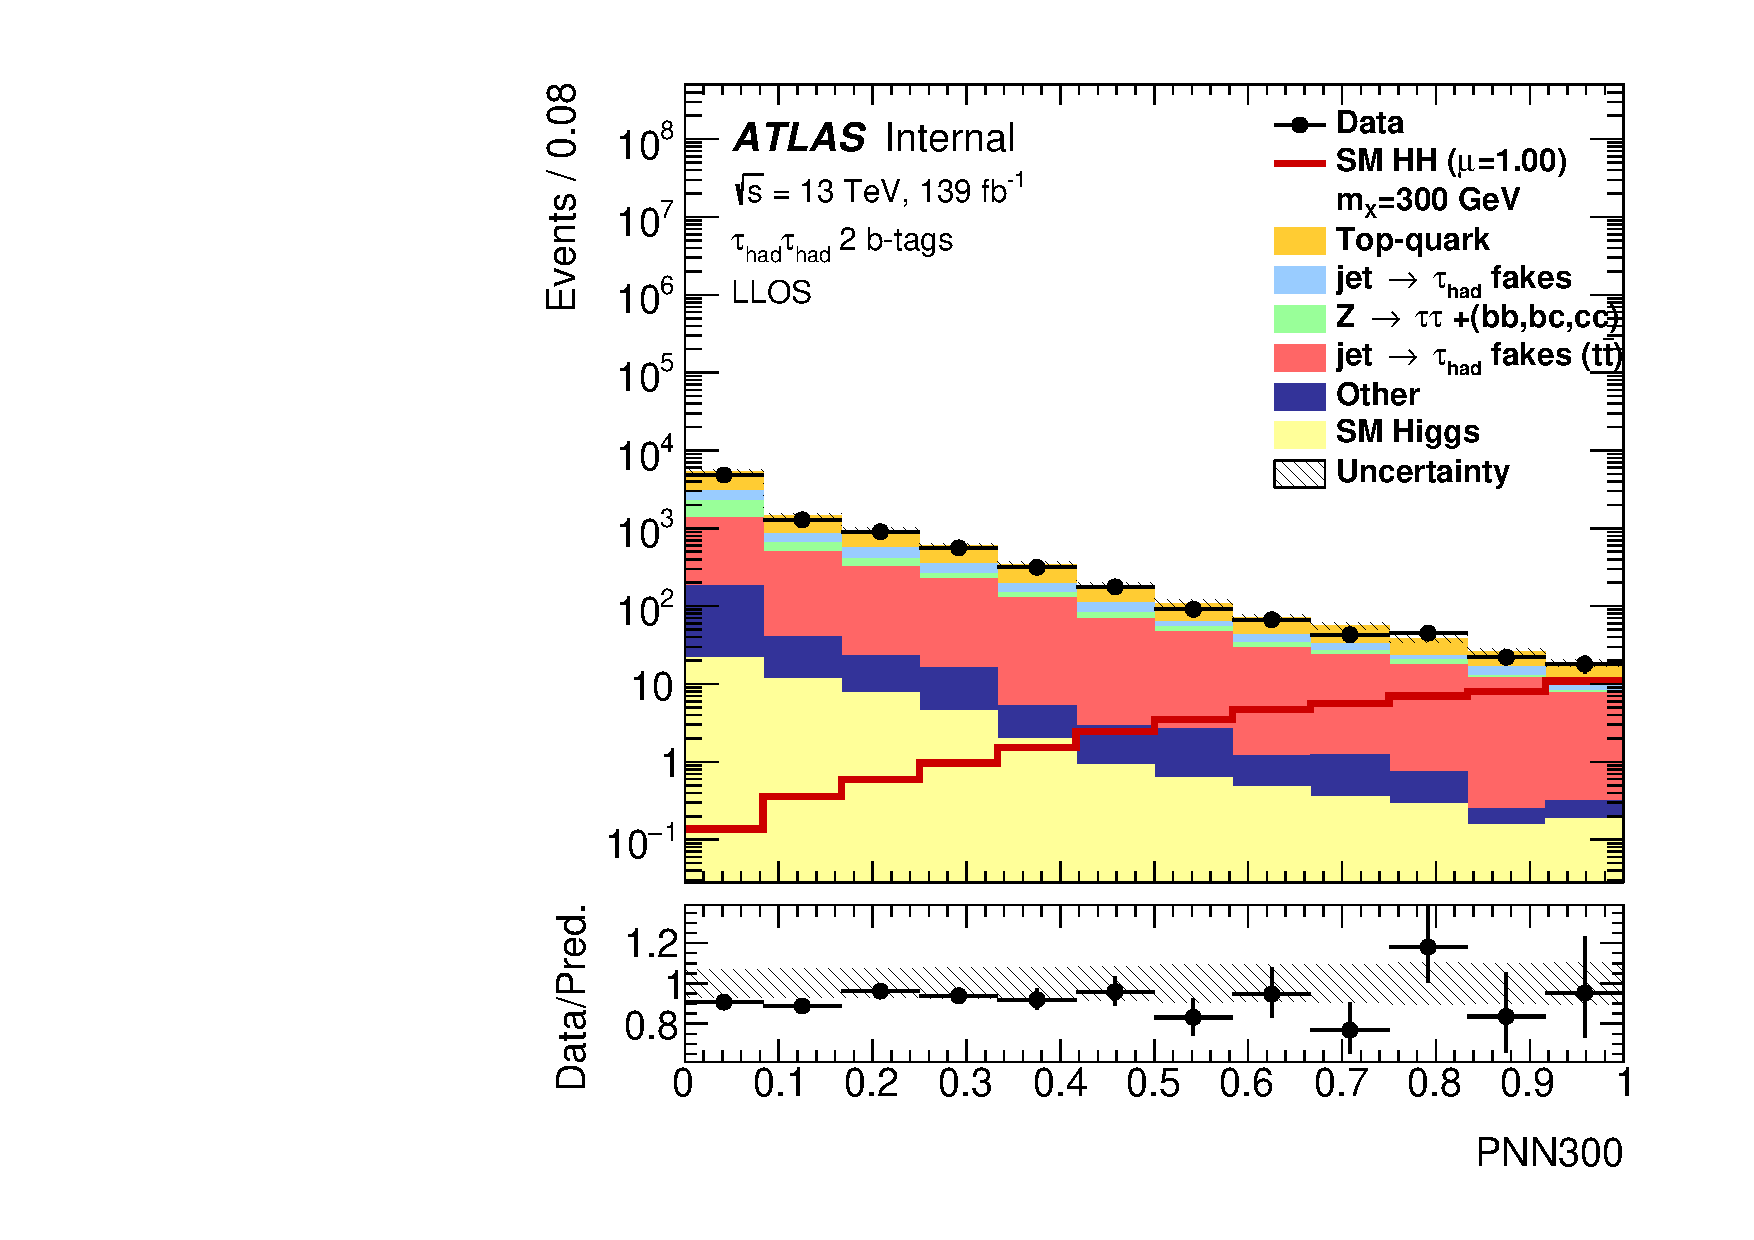
\includegraphics[width=.45\textwidth]{figures/results/HH/HadHad/HadHadFit01062021/MVA/prefit/Region_BMin0_incJet1_distPNN300_J2_Y2015_DLLOS_T2_SpcTauHH_L0_Prefitlog.pdf}
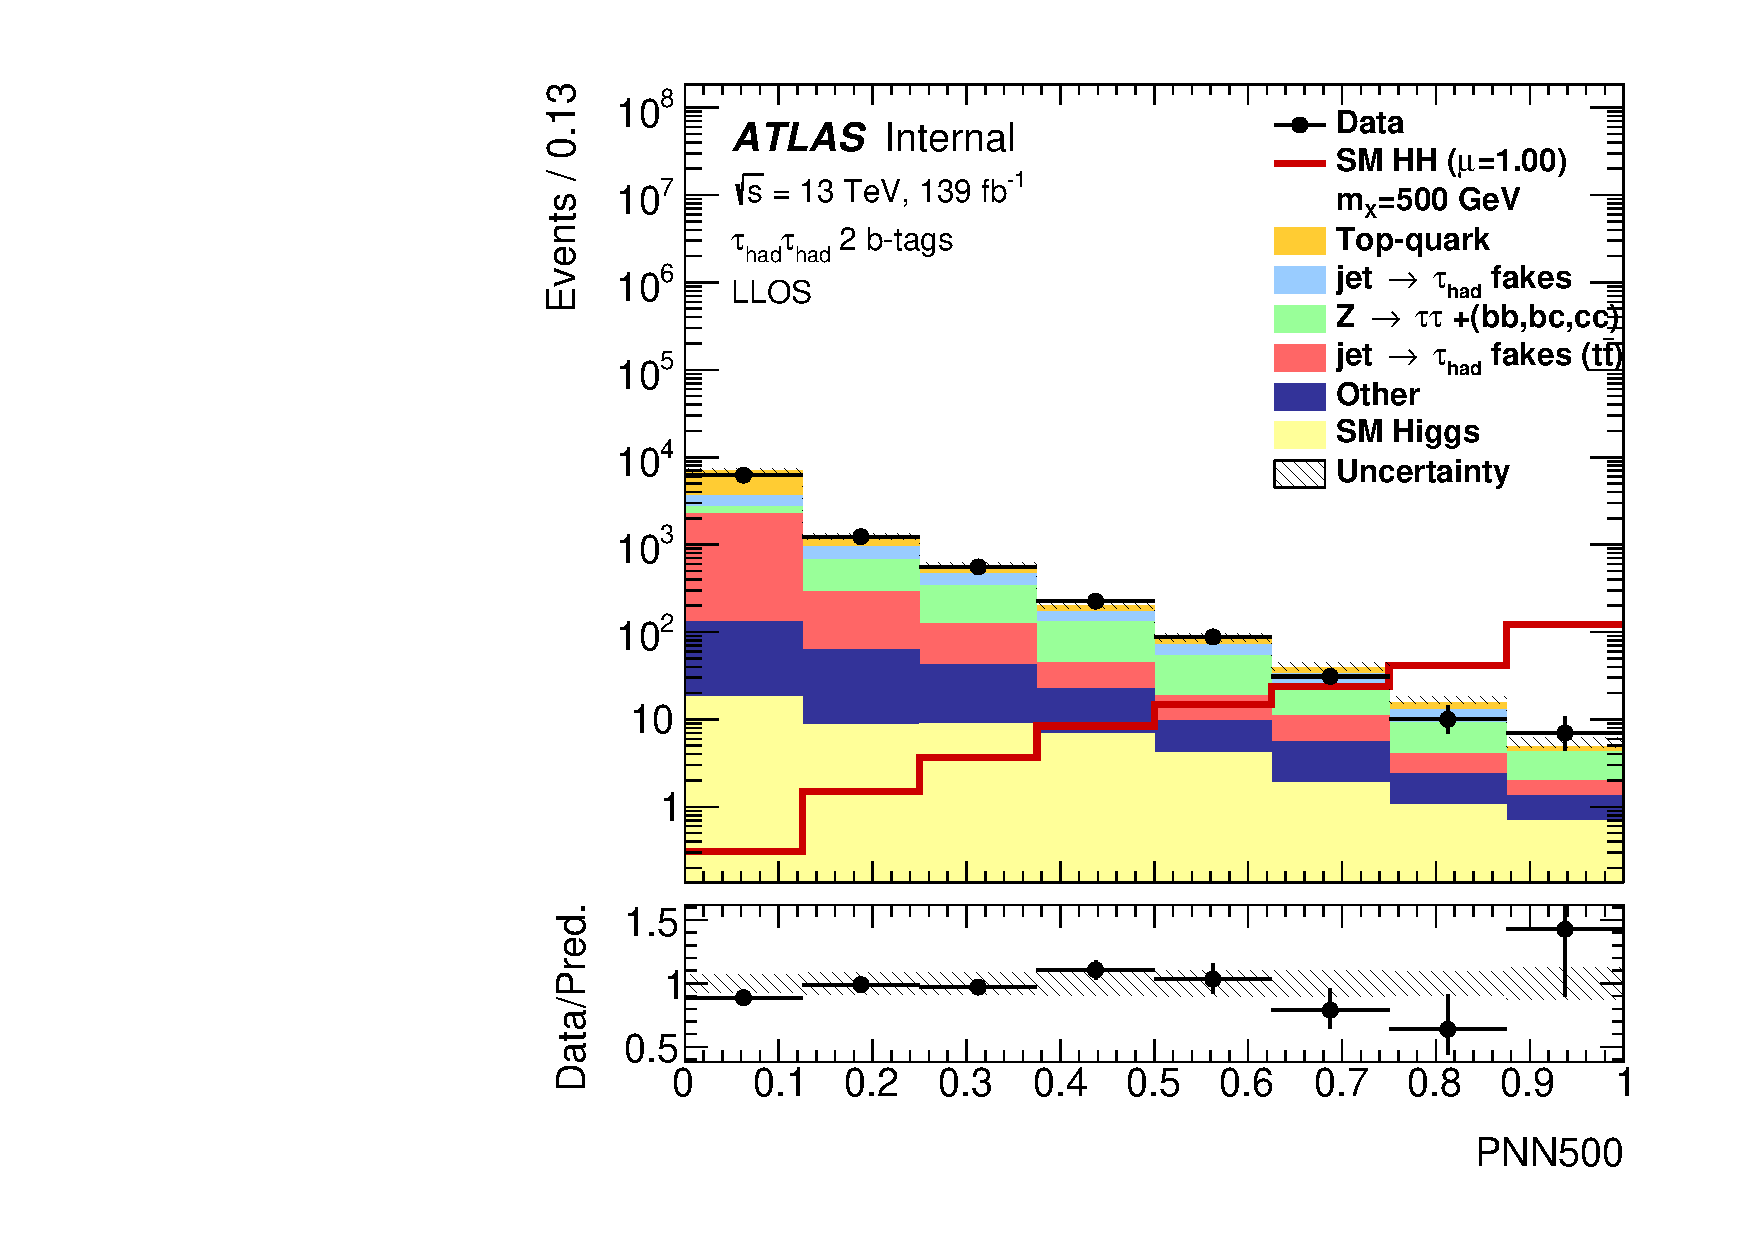
\includegraphics[width=.45\textwidth]{figures/results/HH/HadHad/HadHadFit01062021/MVA/prefit/Region_BMin0_incJet1_distPNN500_J2_Y2015_DLLOS_T2_SpcTauHH_L0_Prefitlog.pdf}\\
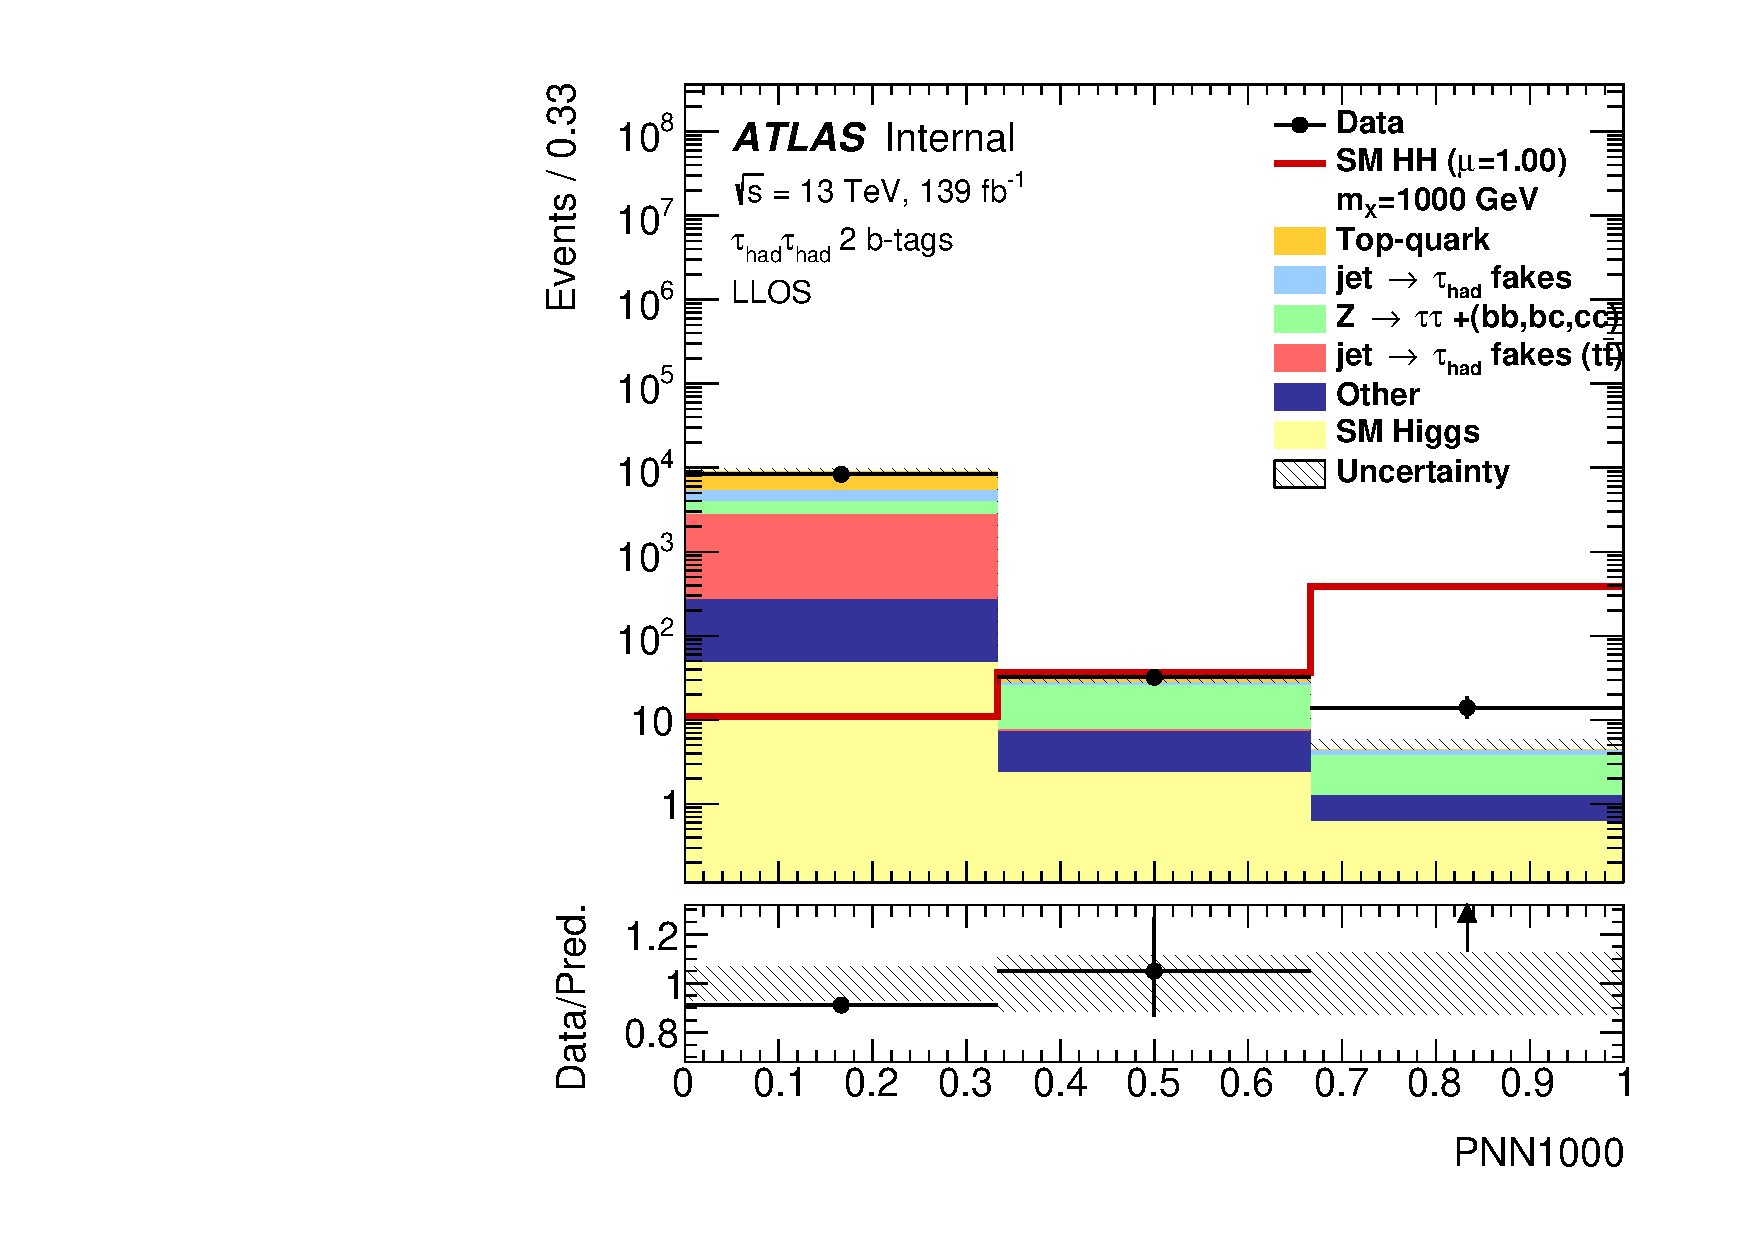
\includegraphics[width=.45\textwidth]{figures/results/HH/HadHad/HadHadFit01062021/MVA/prefit/Region_BMin0_incJet1_distPNN1000_J2_Y2015_DLLOS_T2_SpcTauHH_L0_Prefitlog.pdf}
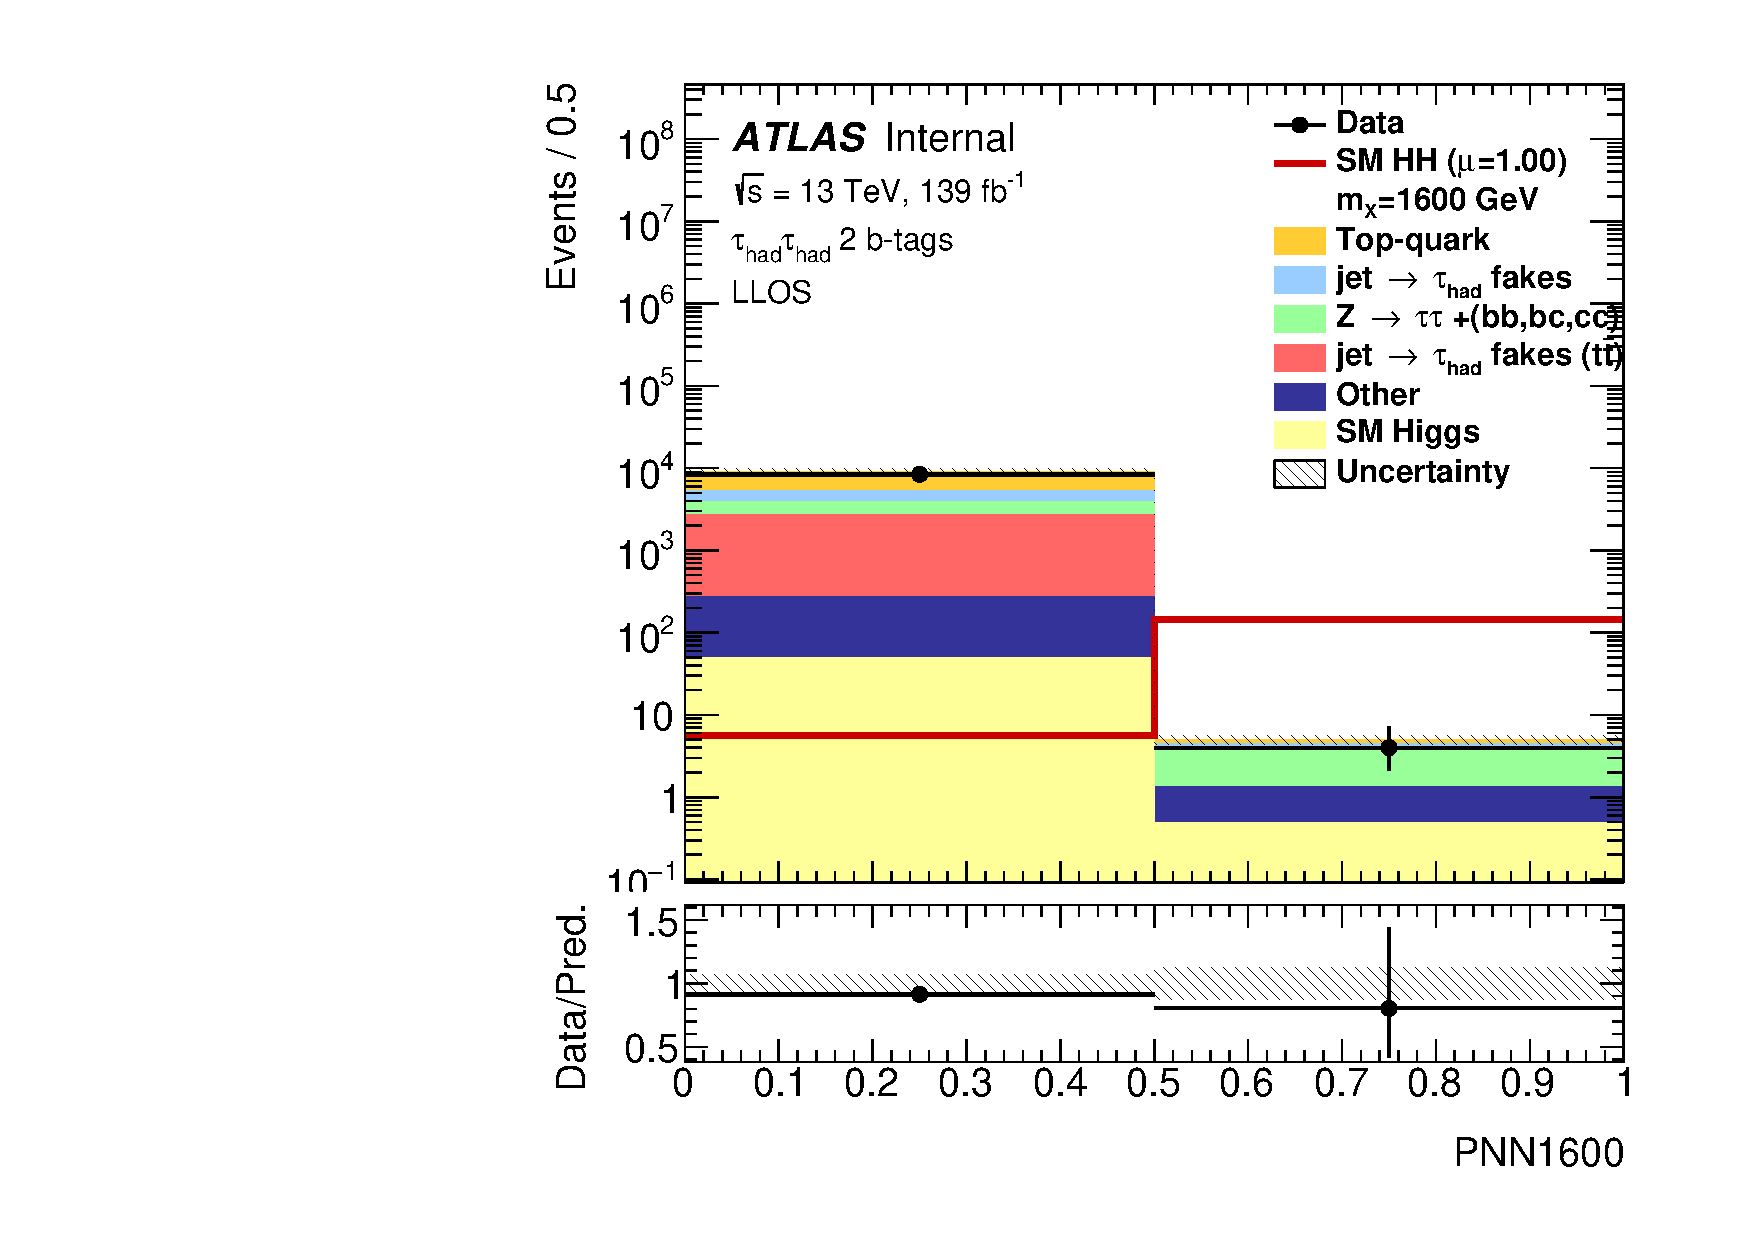
\includegraphics[width=.45\textwidth]{figures/results/HH/HadHad/HadHadFit01062021/MVA/prefit/Region_BMin0_incJet1_distPNN1600_J2_Y2015_DLLOS_T2_SpcTauHH_L0_Prefitlog.pdf}
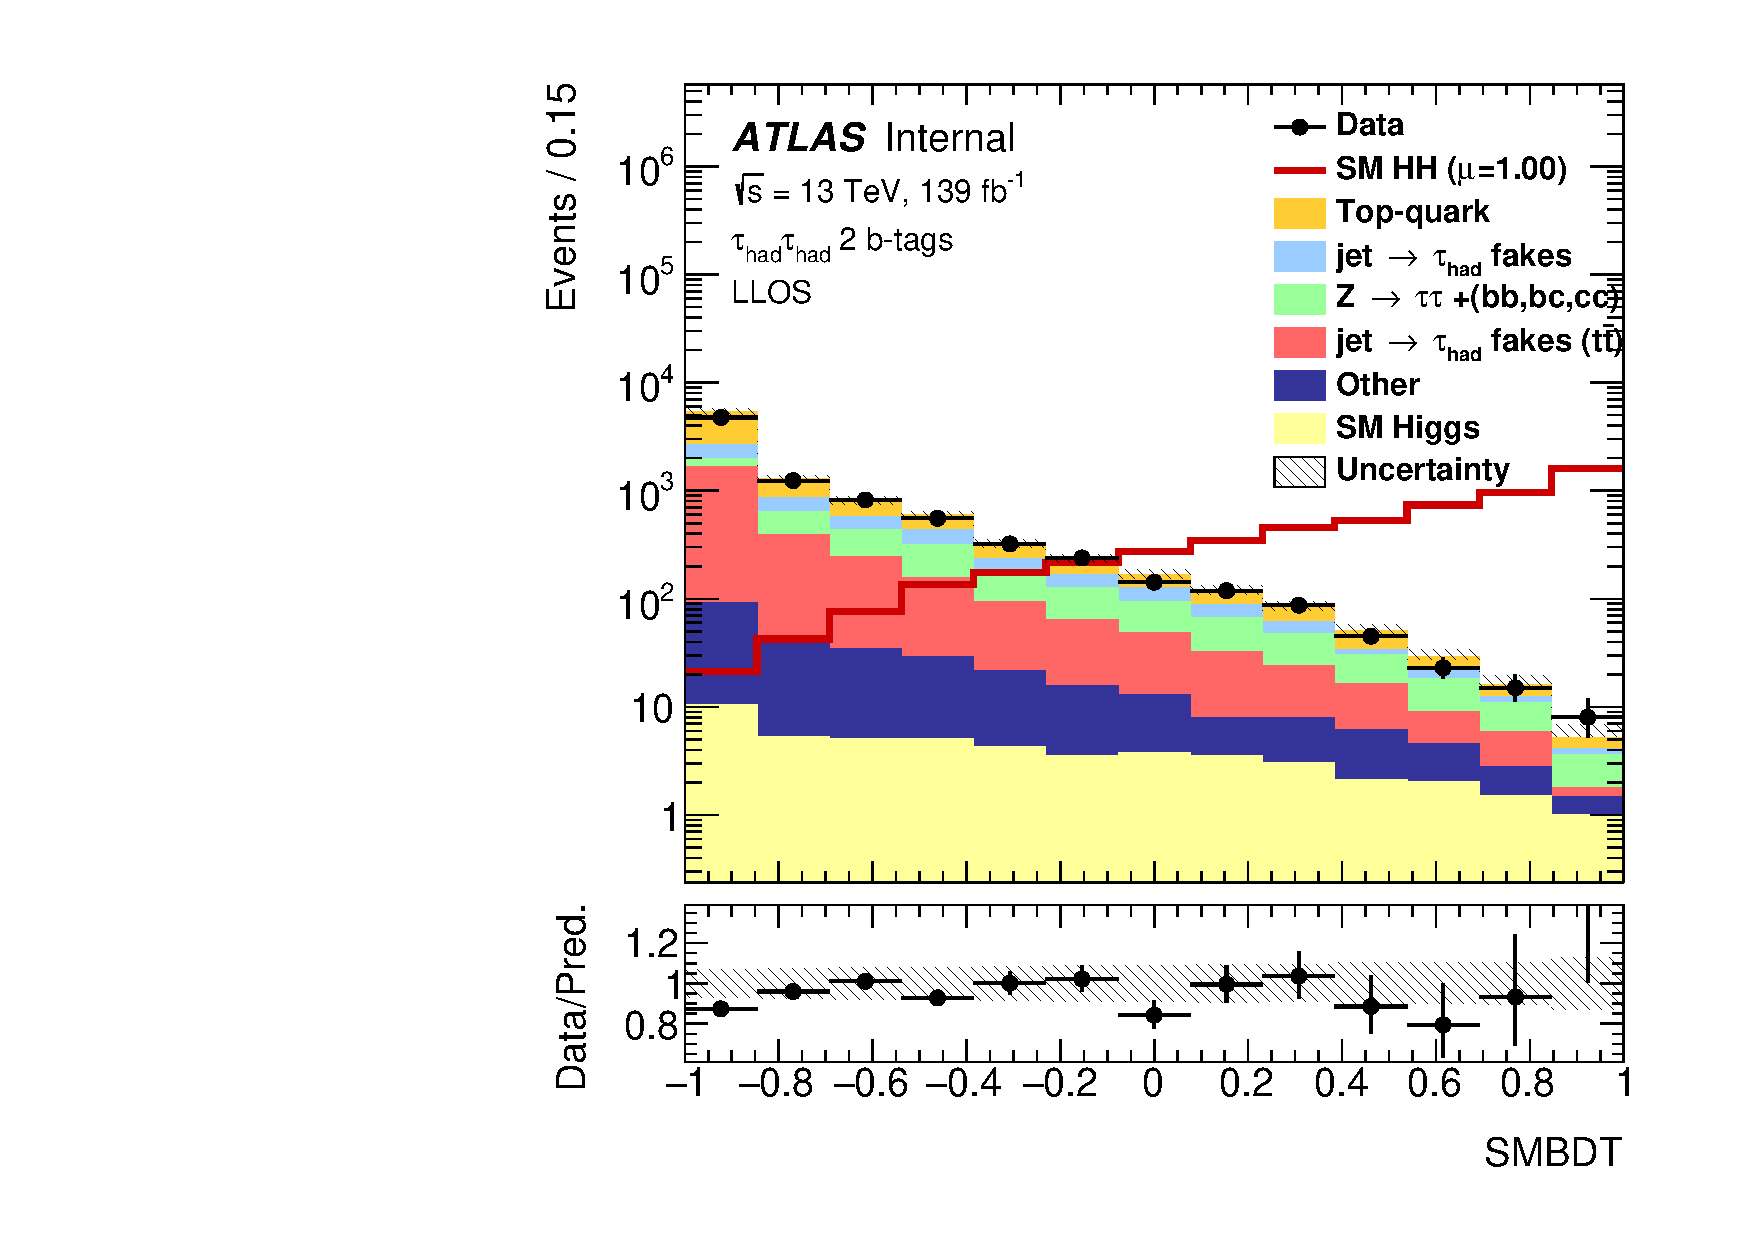
\includegraphics[width=.45\textwidth]{figures/results/HH/HadHad/HadHadFit01062021/MVA/prefit/Region_BMin0_incJet1_distSMBDT_J2_Y2015_DLLOS_T2_SpcTauHH_L0_Prefitlog.pdf}\\
\caption{Pre-fit PNN score distributions for the $300, 500, 1000, 1600$ GeV mass points and pre-fit SM BDT distribution in the di-Higgs $bb\tau_{had}\tau_{had}$ signal region. The uncertainty band includes all uncertainties. The signal is normalised to the input cross section. (Inputs from 2021\textunderscore 05\textunderscore 25)}
\label{fig:HadHadPreselectionPNNScoreDistributions}
\end{figure}

\begin{figure}
\centering
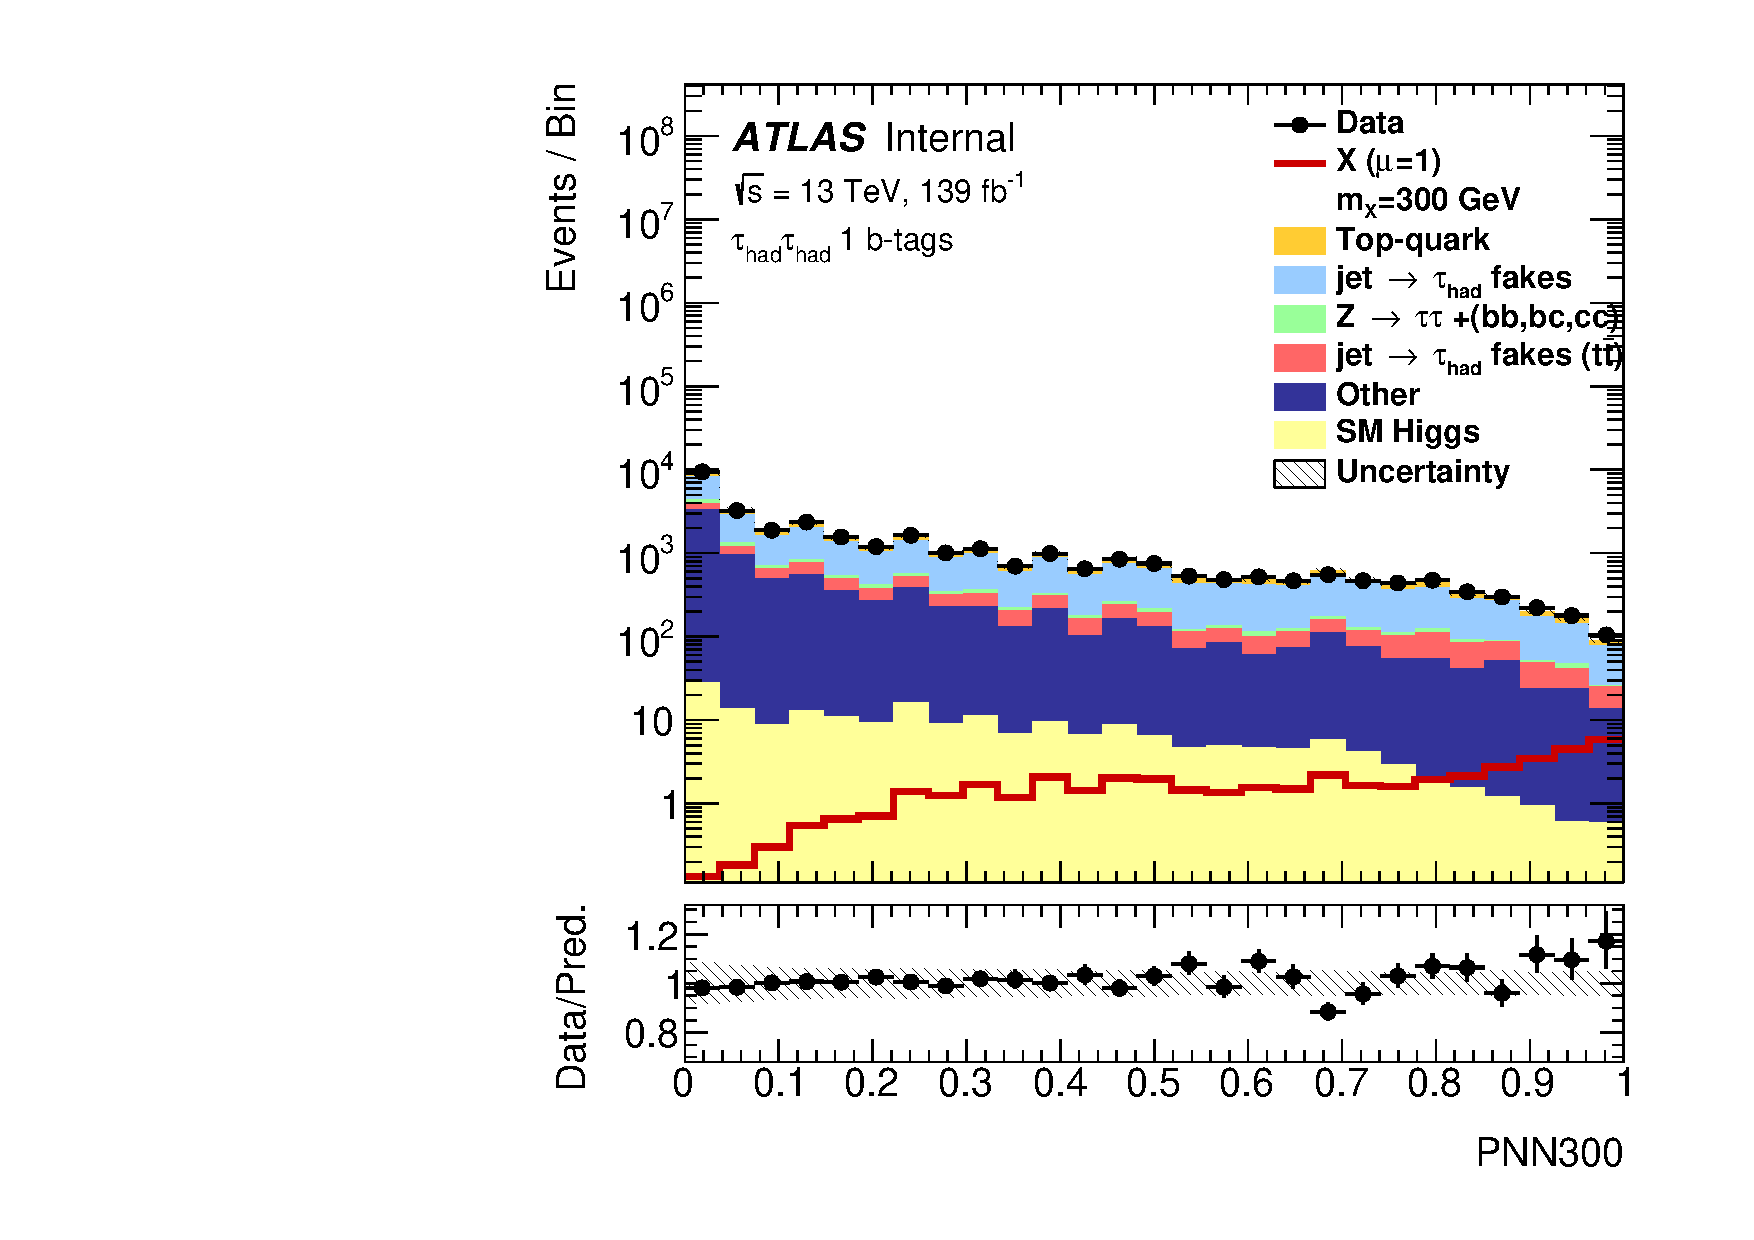
\includegraphics[width=.45\textwidth]{figures/mva/HH/HadHad/Region_BMin0_incJet1_distPNN300_J2_Y2015_DLLOS_T1_SpcTauHH_L0_Prefitlog.pdf}
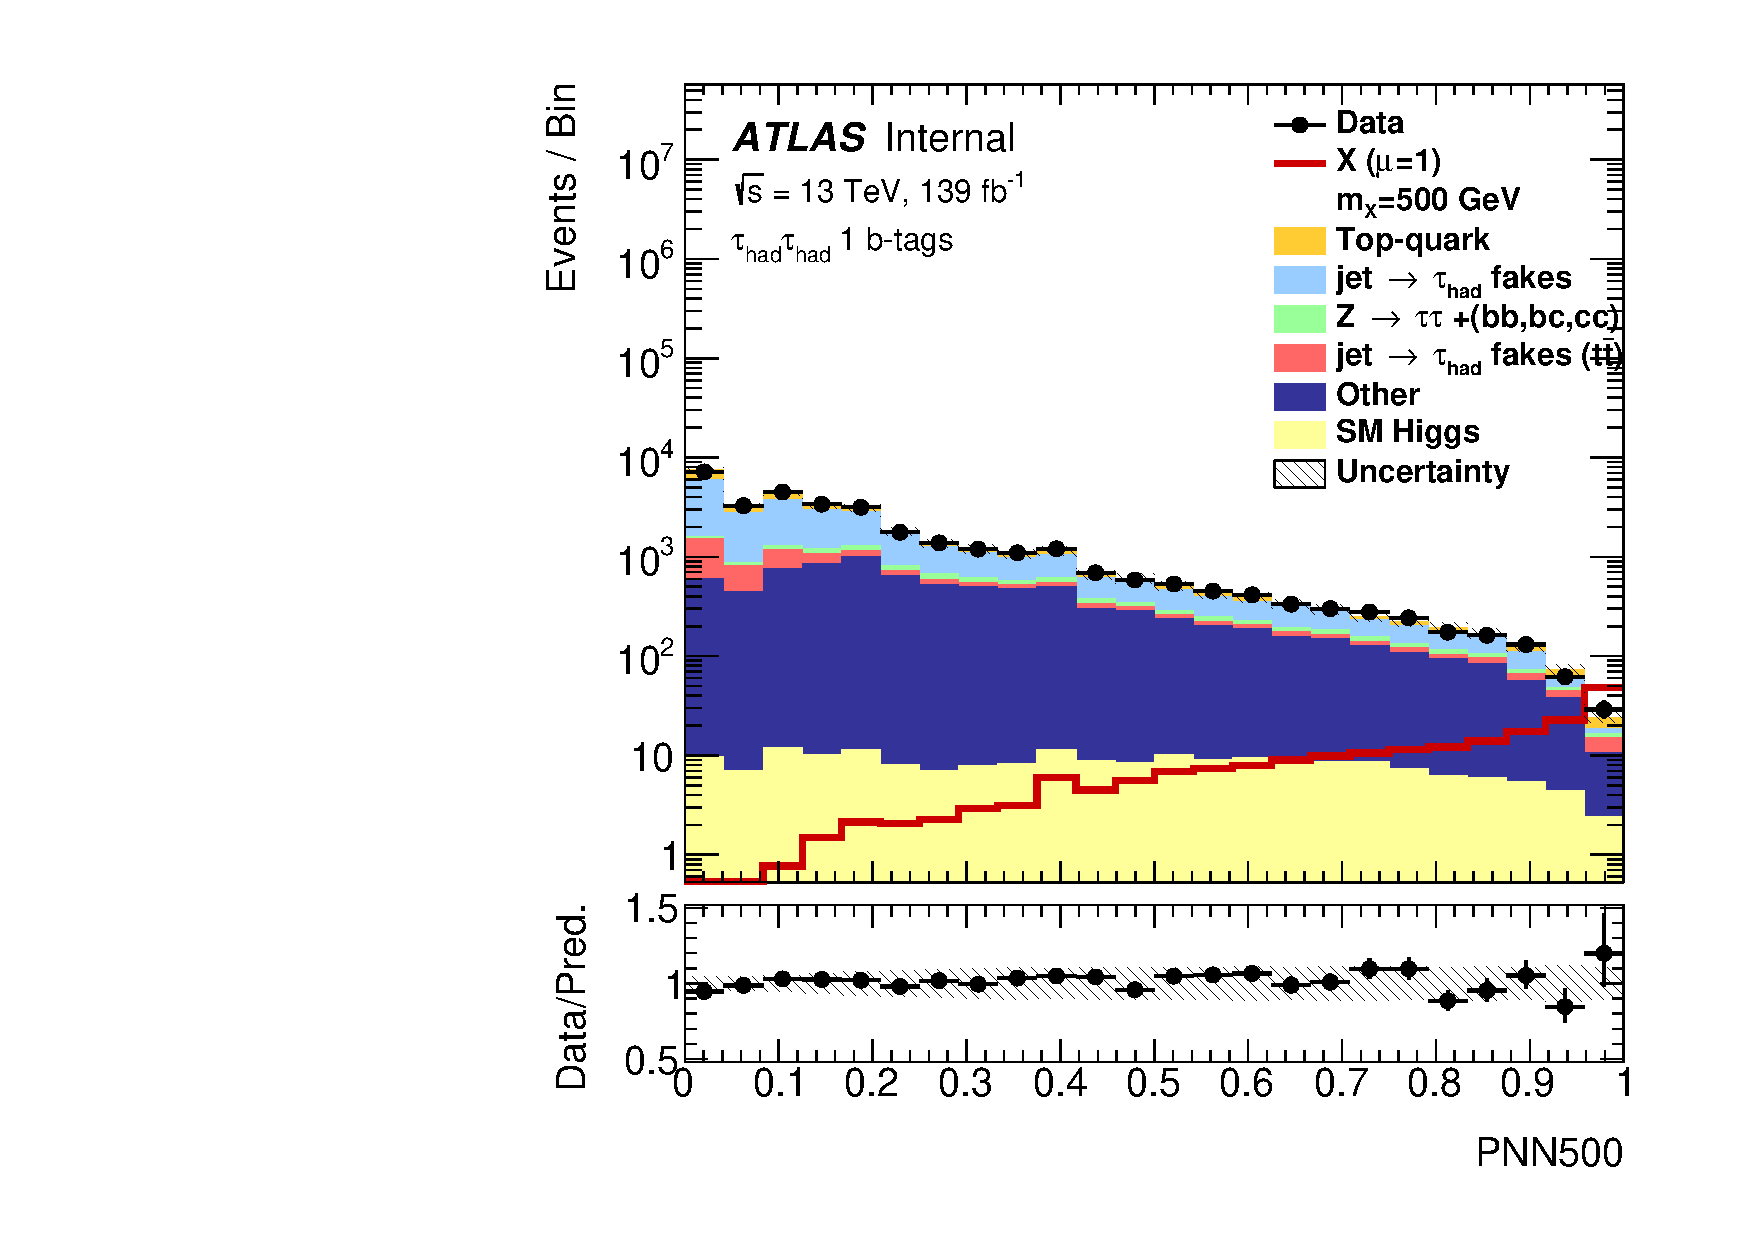
\includegraphics[width=.45\textwidth]{figures/mva/HH/HadHad/Region_BMin0_incJet1_distPNN500_J2_Y2015_DLLOS_T1_SpcTauHH_L0_Prefitlog.pdf}\\
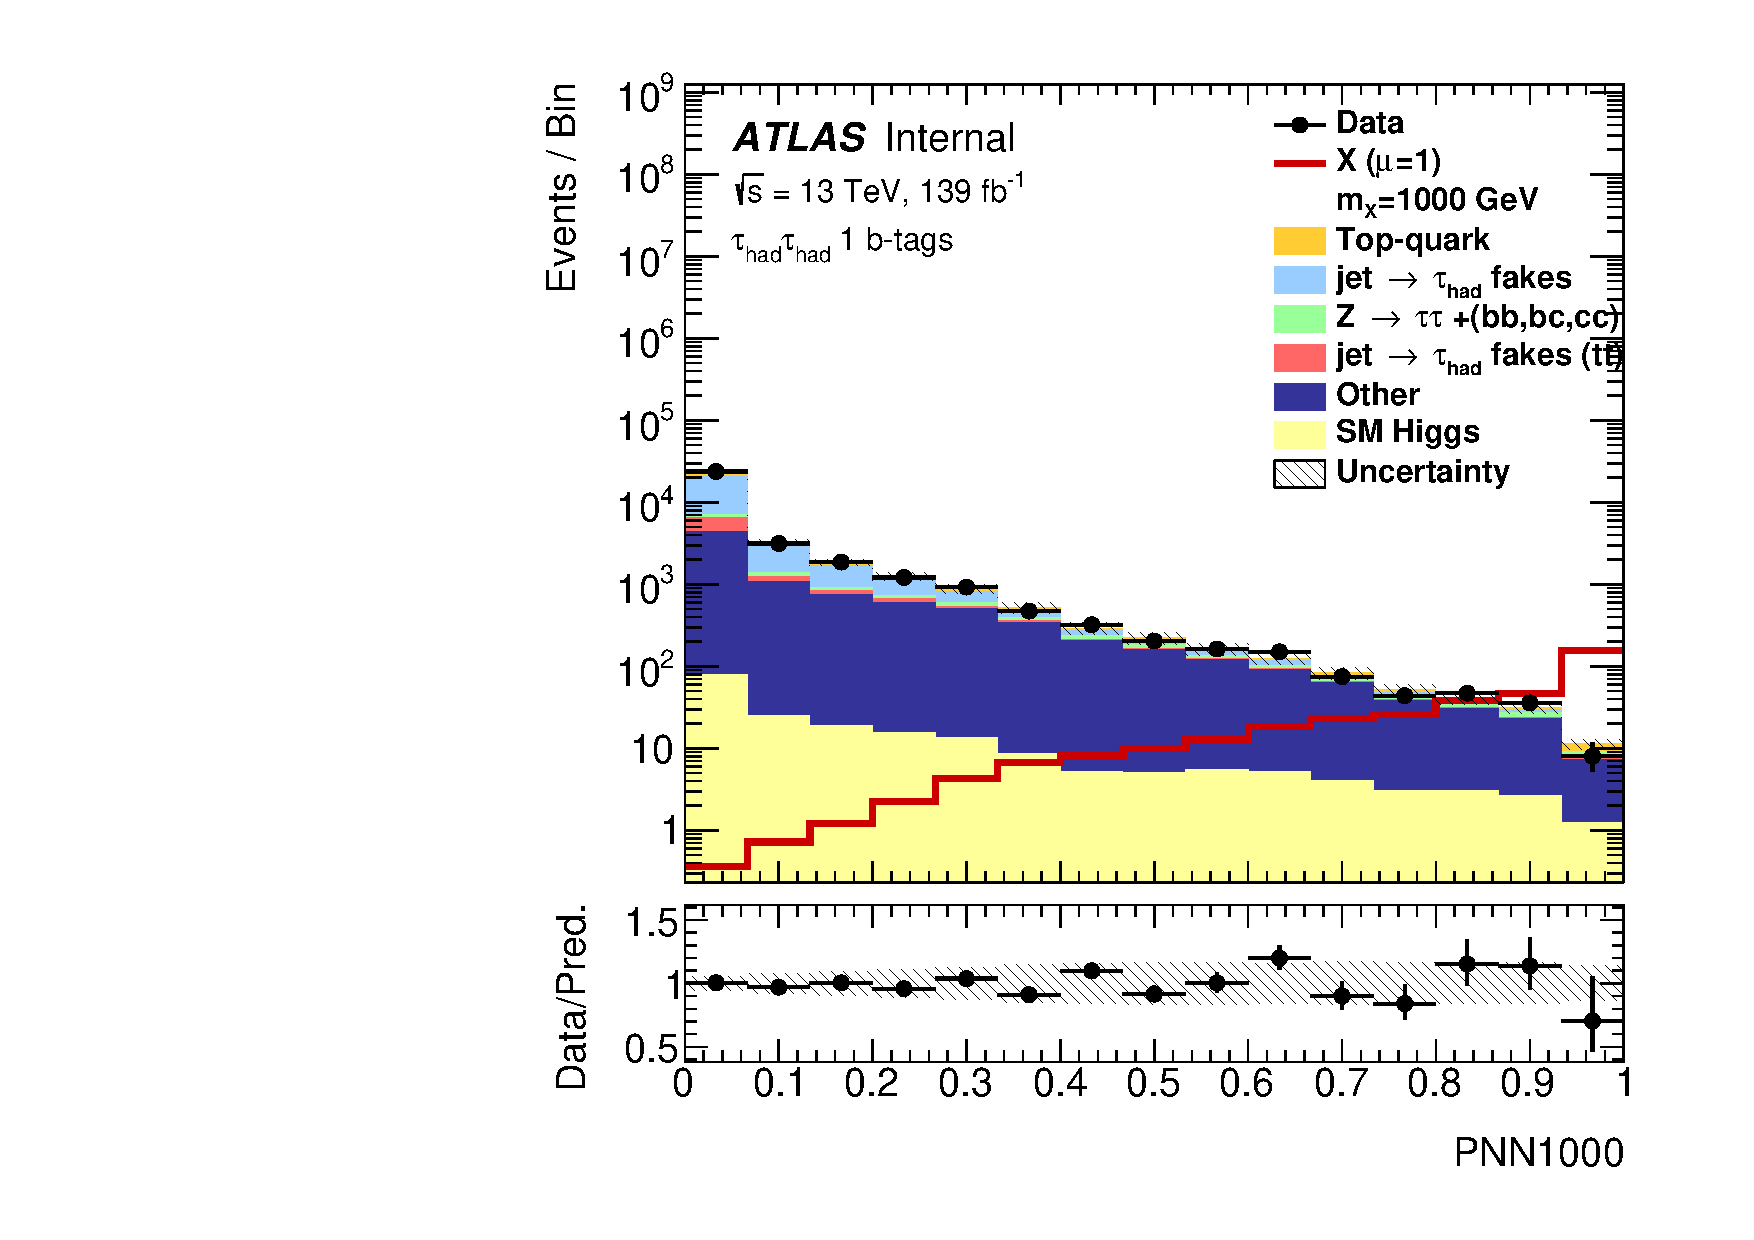
\includegraphics[width=.45\textwidth]{figures/mva/HH/HadHad/Region_BMin0_incJet1_distPNN1000_J2_Y2015_DLLOS_T1_SpcTauHH_L0_Prefitlog.pdf}
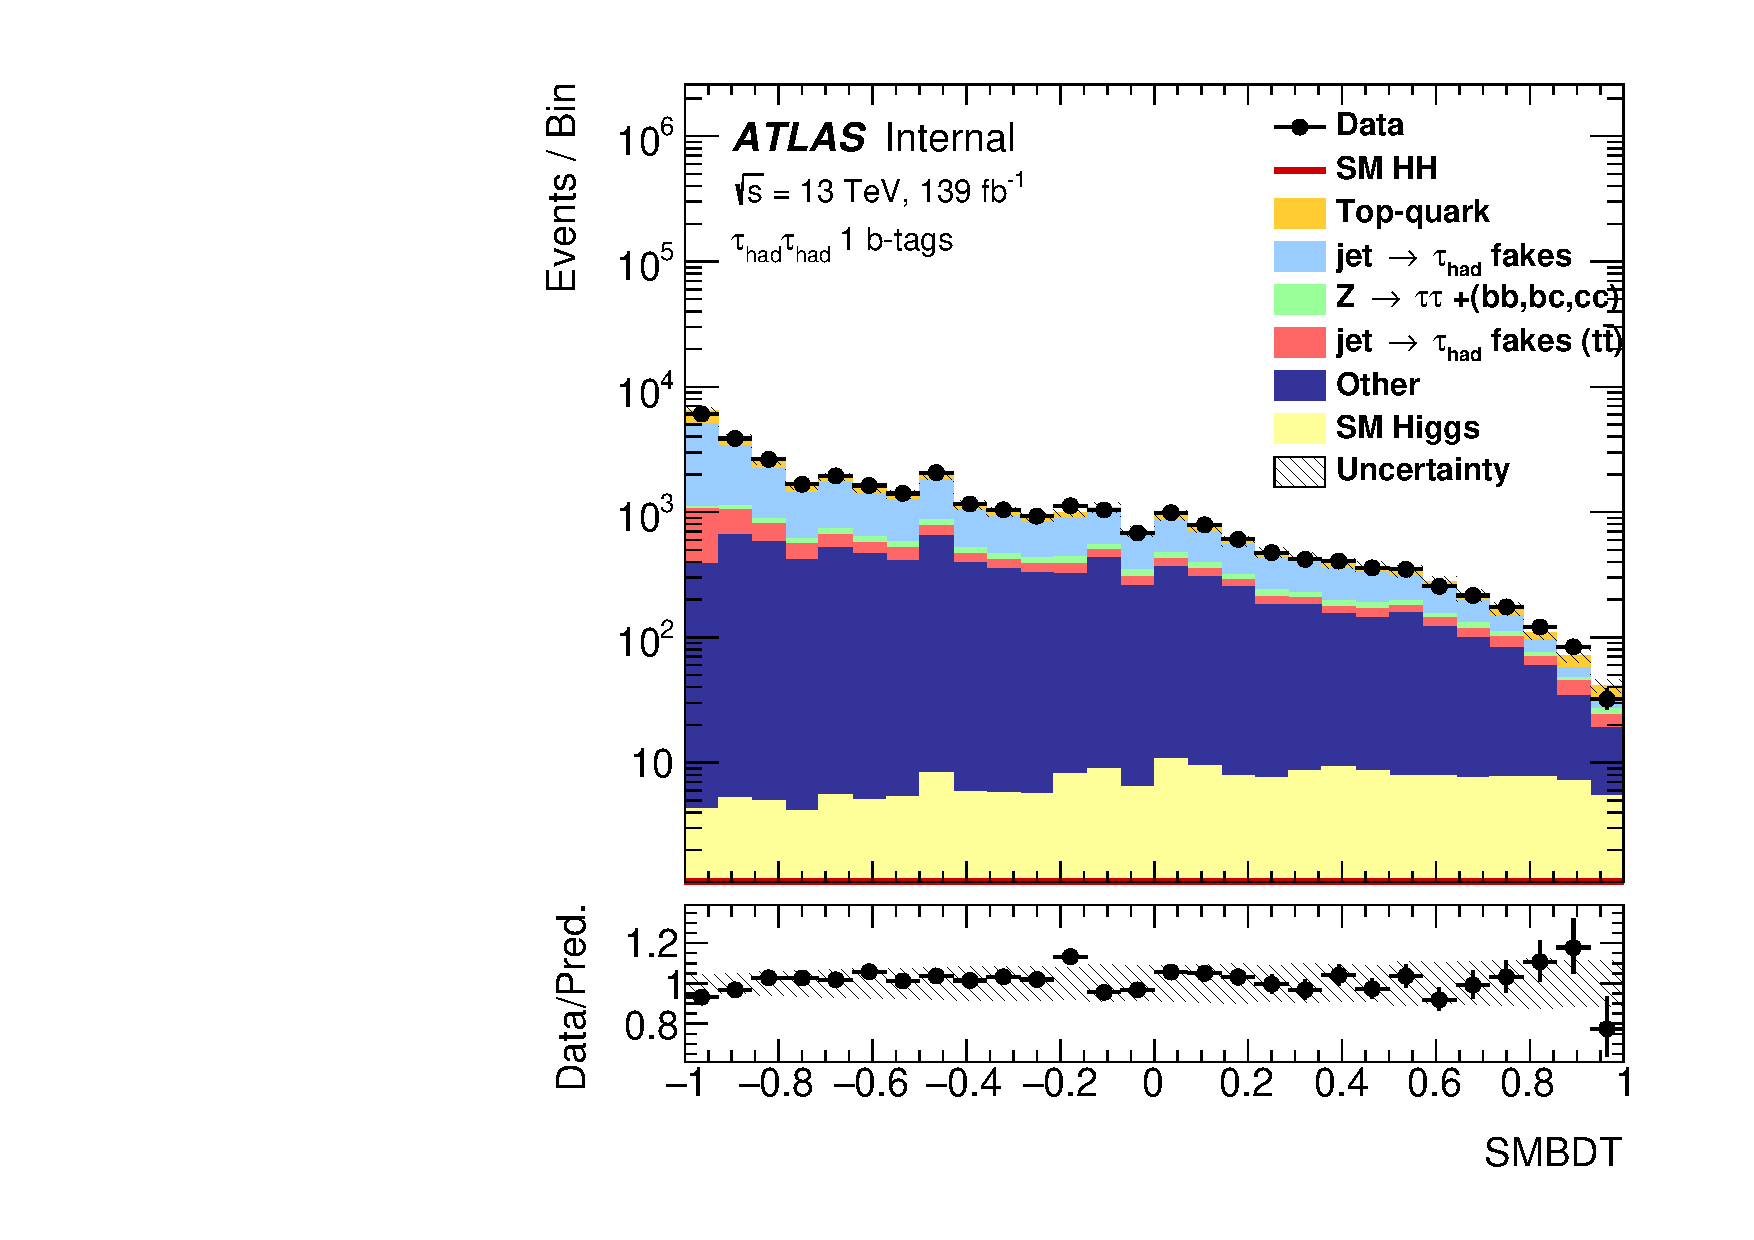
\includegraphics[width=.45\textwidth]{figures/mva/HH/HadHad/Region_BMin0_incJet1_distSMBDT_J2_Y2015_DLLOS_T1_SpcTauHH_L0_Prefitlog.pdf}
\caption{Pre-fit PNN score distributions for the $300, 500, 1000$ GeV mass points and pre-fit SM BDT distribution in the di-Higgs $bb\tau_{had}\tau_{had}$ 1 $b$-tag validation region. The signal is normalised to the input cross section. (Inputs from 2020\textunderscore 11\textunderscore 26)}
\label{fig:HadHadPreselectionPNNScoreDistributions1bTag}
\end{figure}

\begin{figure}
\centering
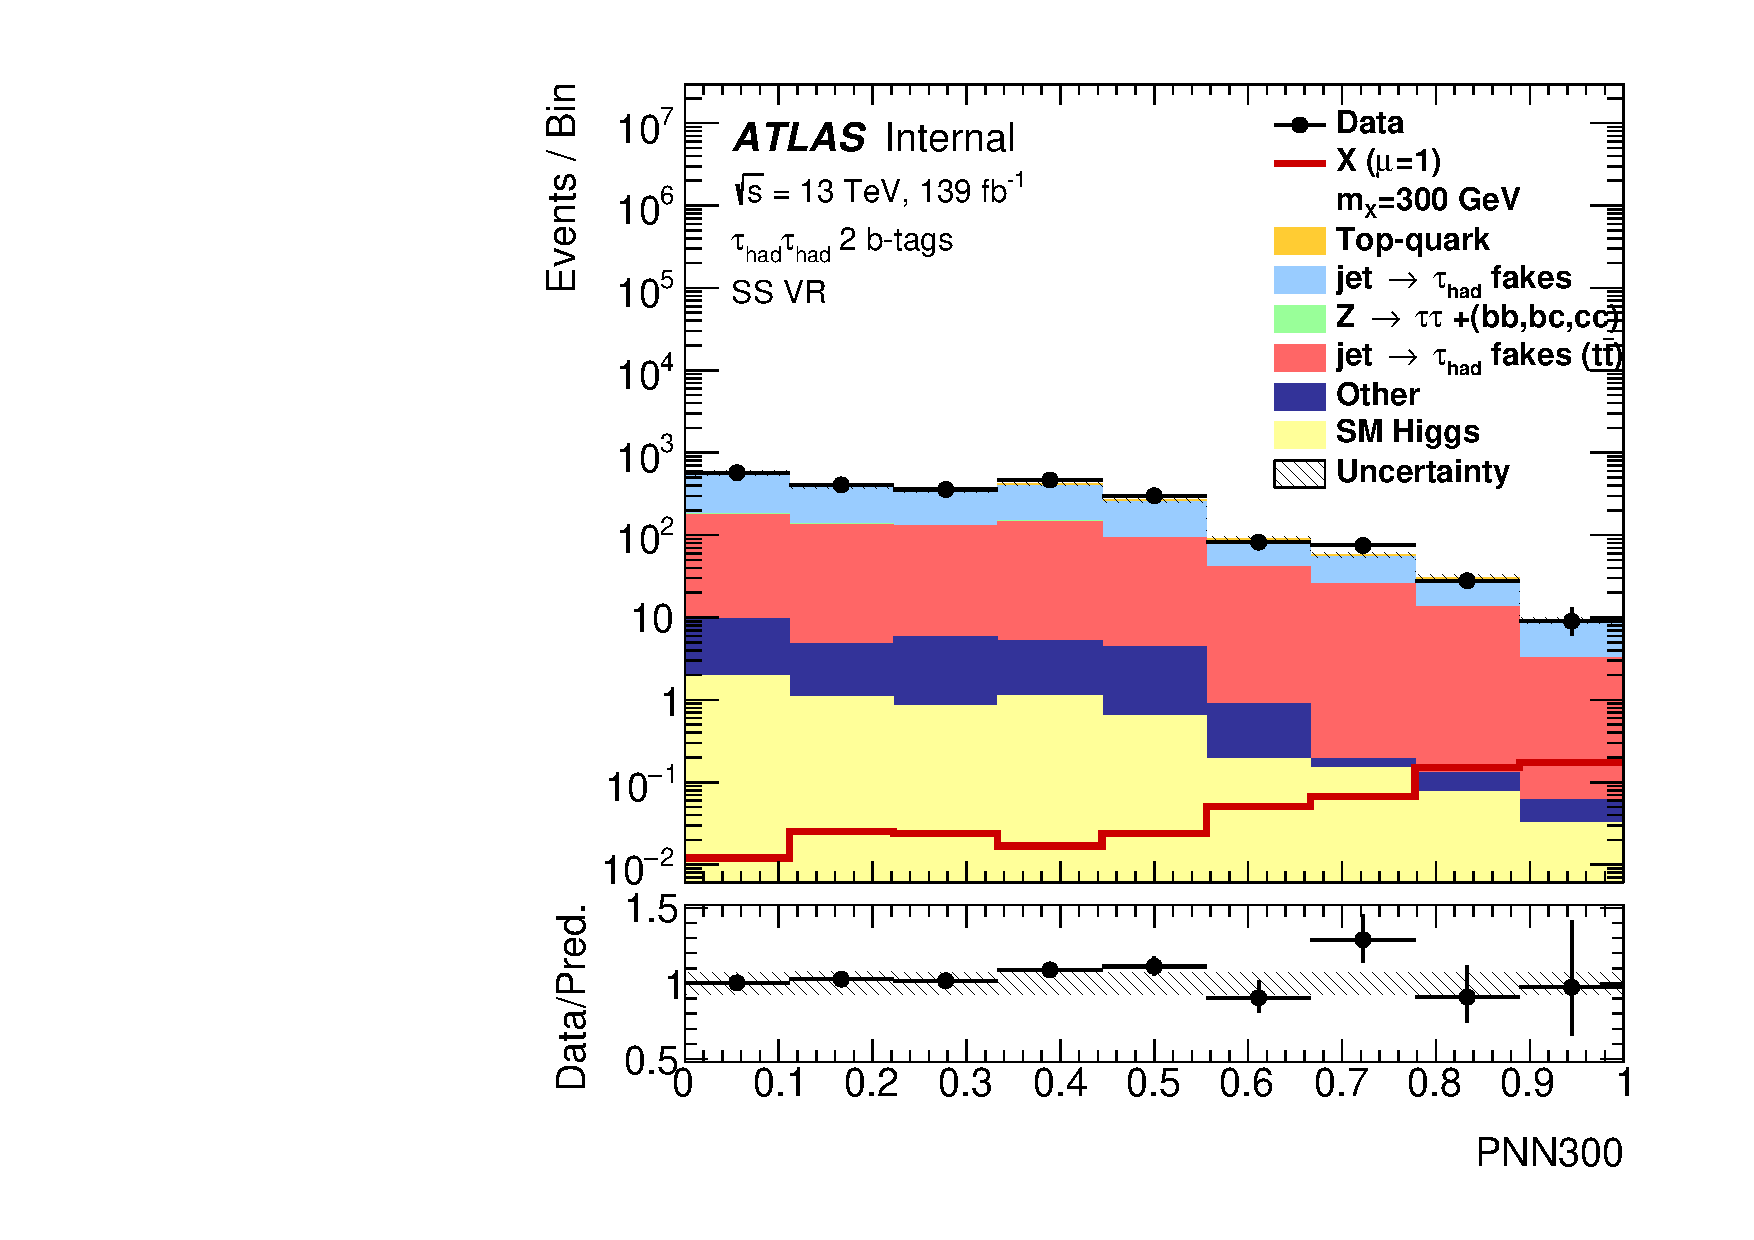
\includegraphics[width=.45\textwidth]{figures/mva/HH/HadHad/Region_BMin0_incJet1_distPNN300_J2_Y2015_DLLSS_T2_SpcTauHH_L0_Prefitlog.pdf}
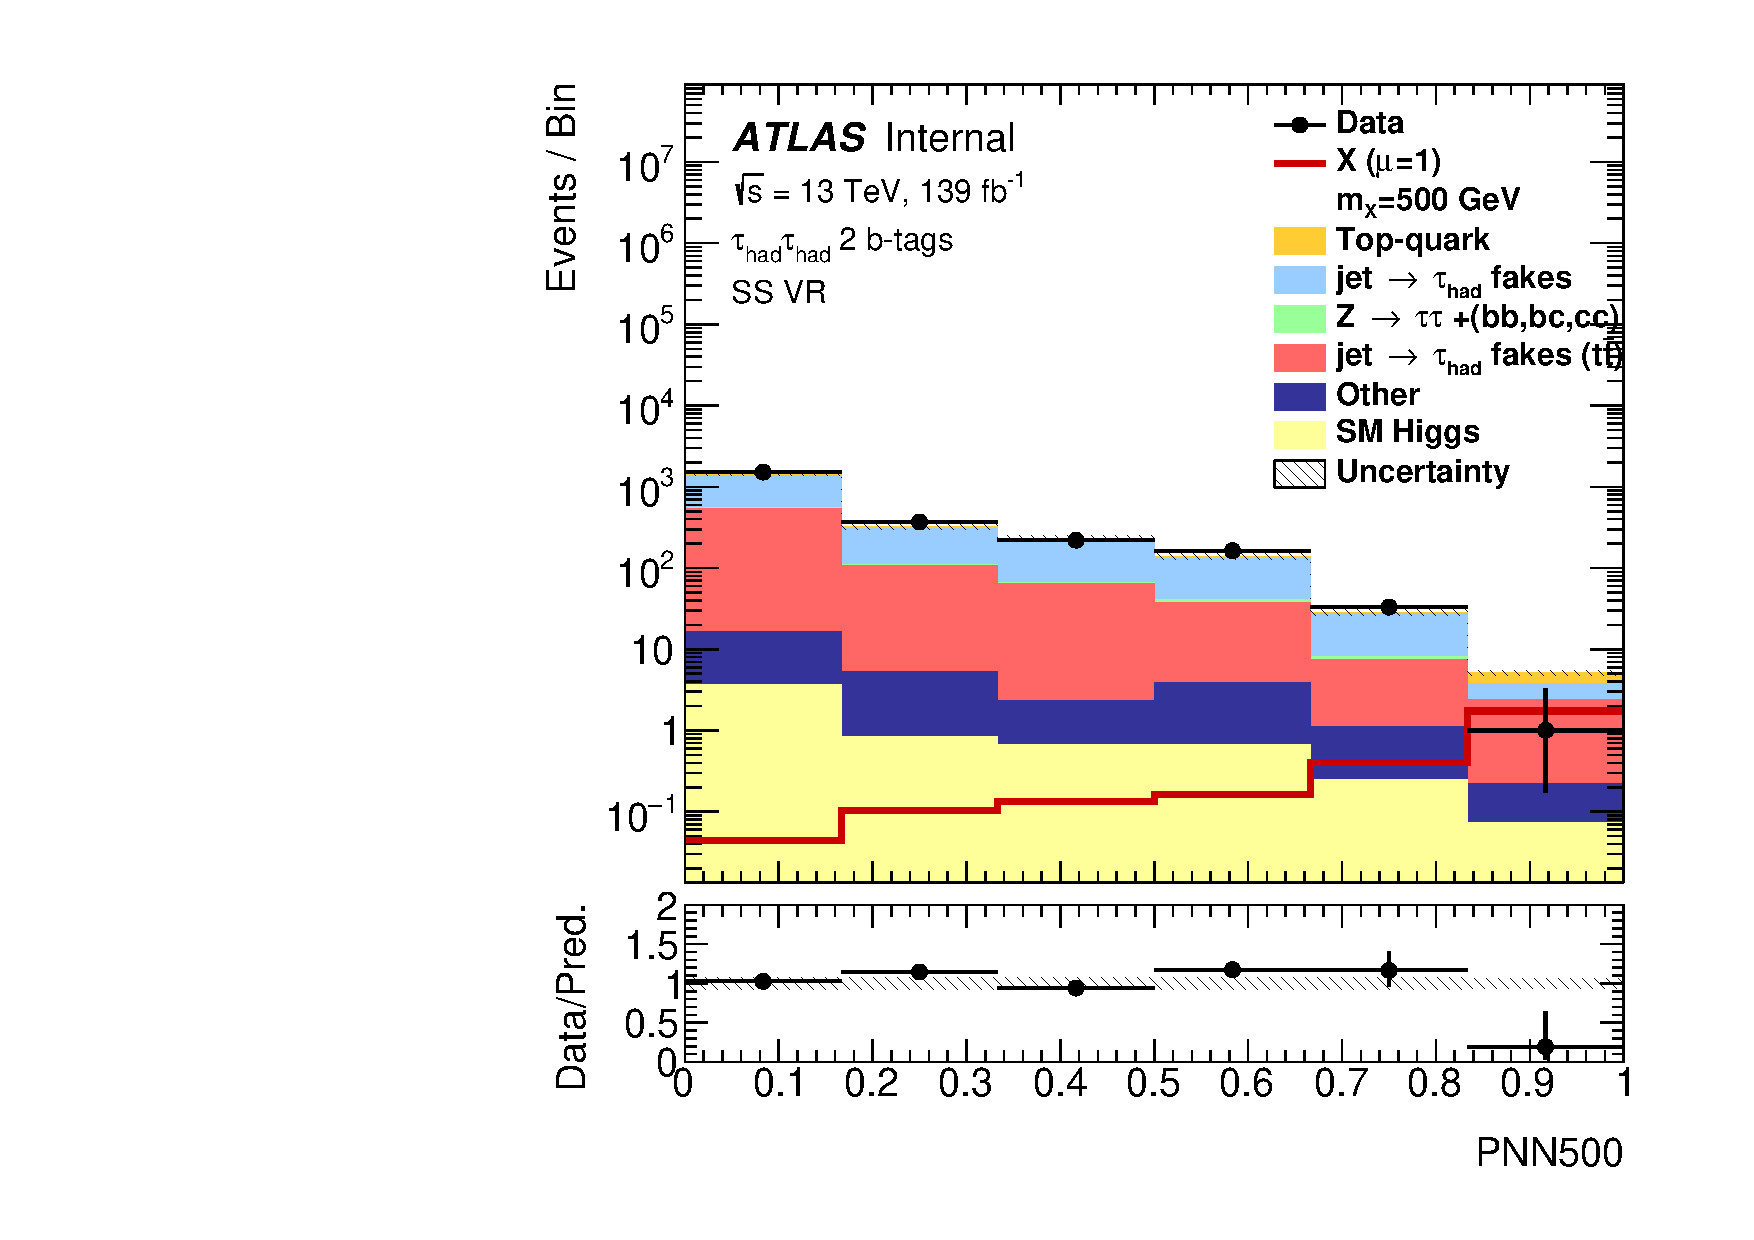
\includegraphics[width=.45\textwidth]{figures/mva/HH/HadHad/Region_BMin0_incJet1_distPNN500_J2_Y2015_DLLSS_T2_SpcTauHH_L0_Prefitlog.pdf}\\
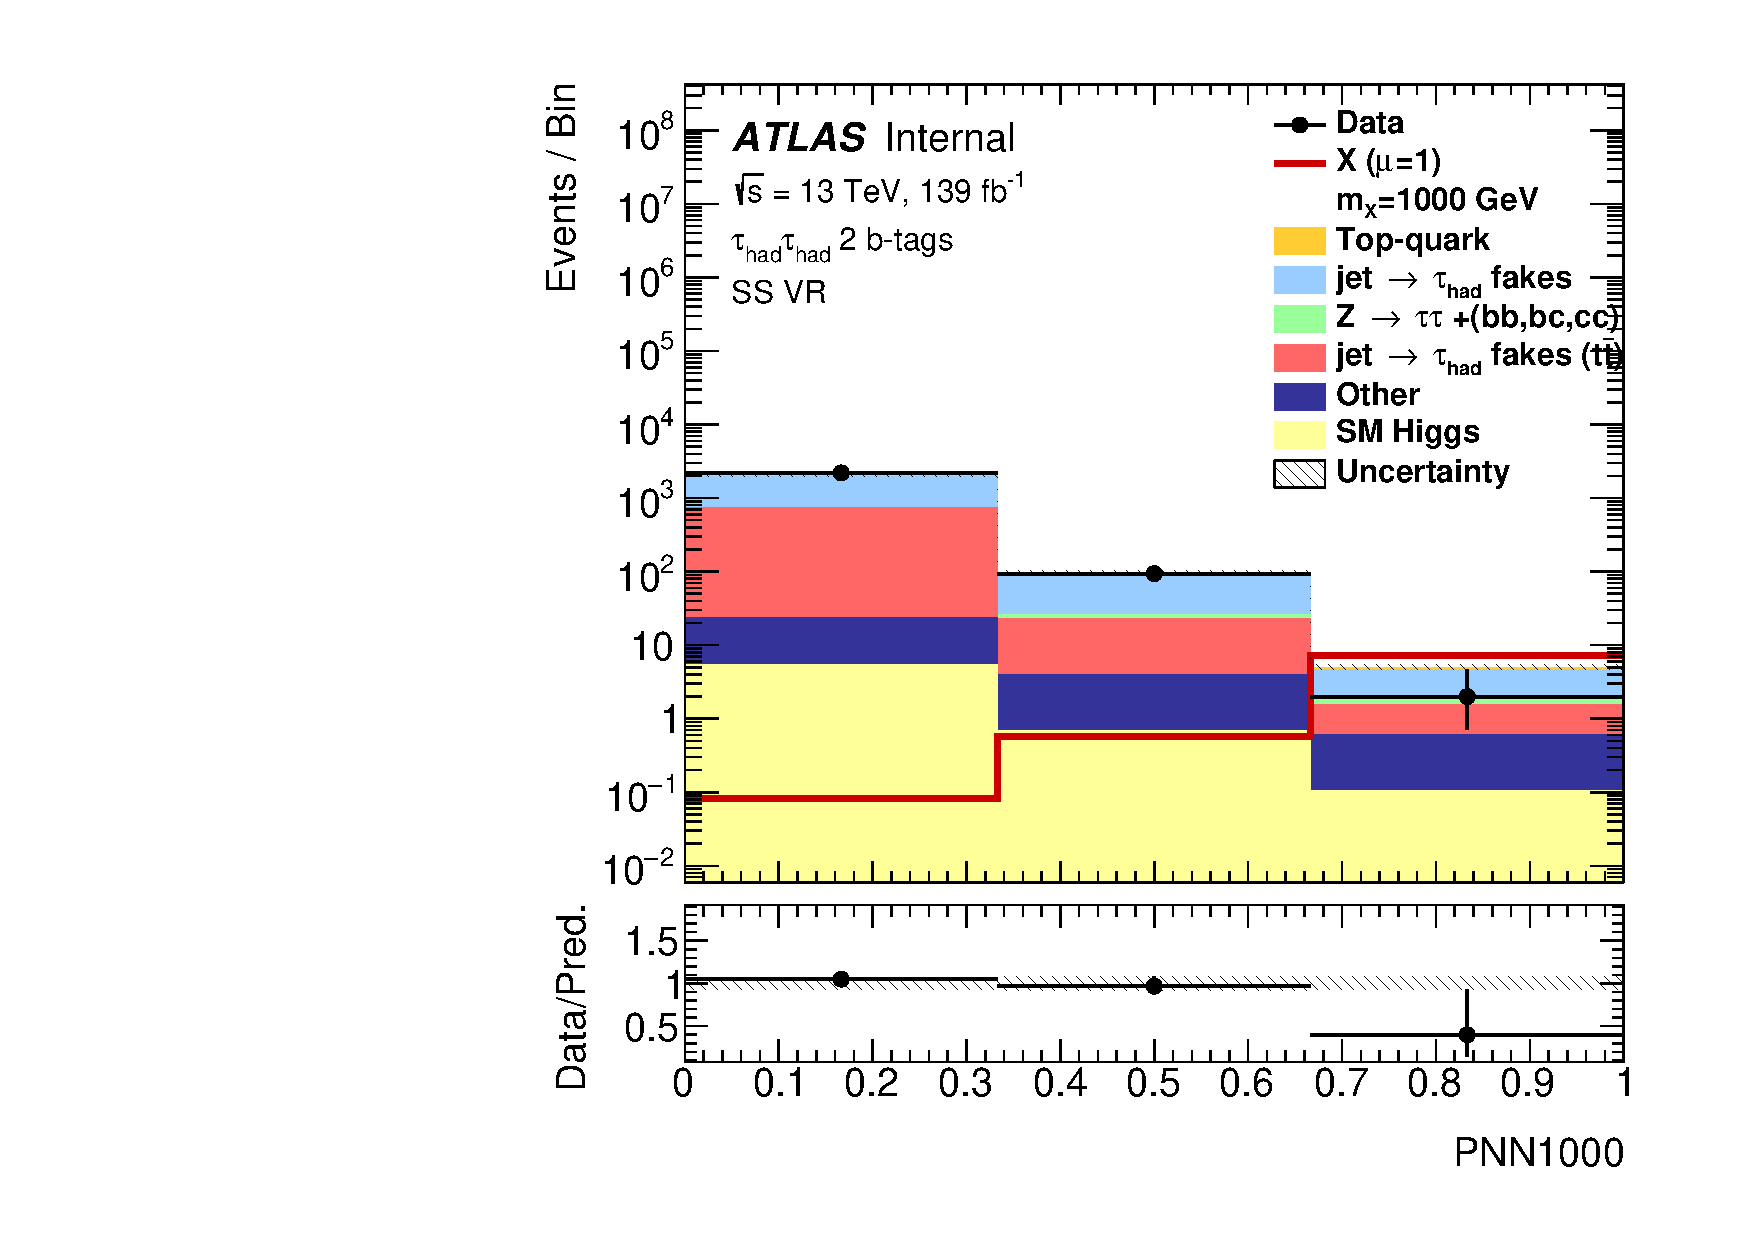
\includegraphics[width=.45\textwidth]{figures/mva/HH/HadHad/Region_BMin0_incJet1_distPNN1000_J2_Y2015_DLLSS_T2_SpcTauHH_L0_Prefitlog.pdf}
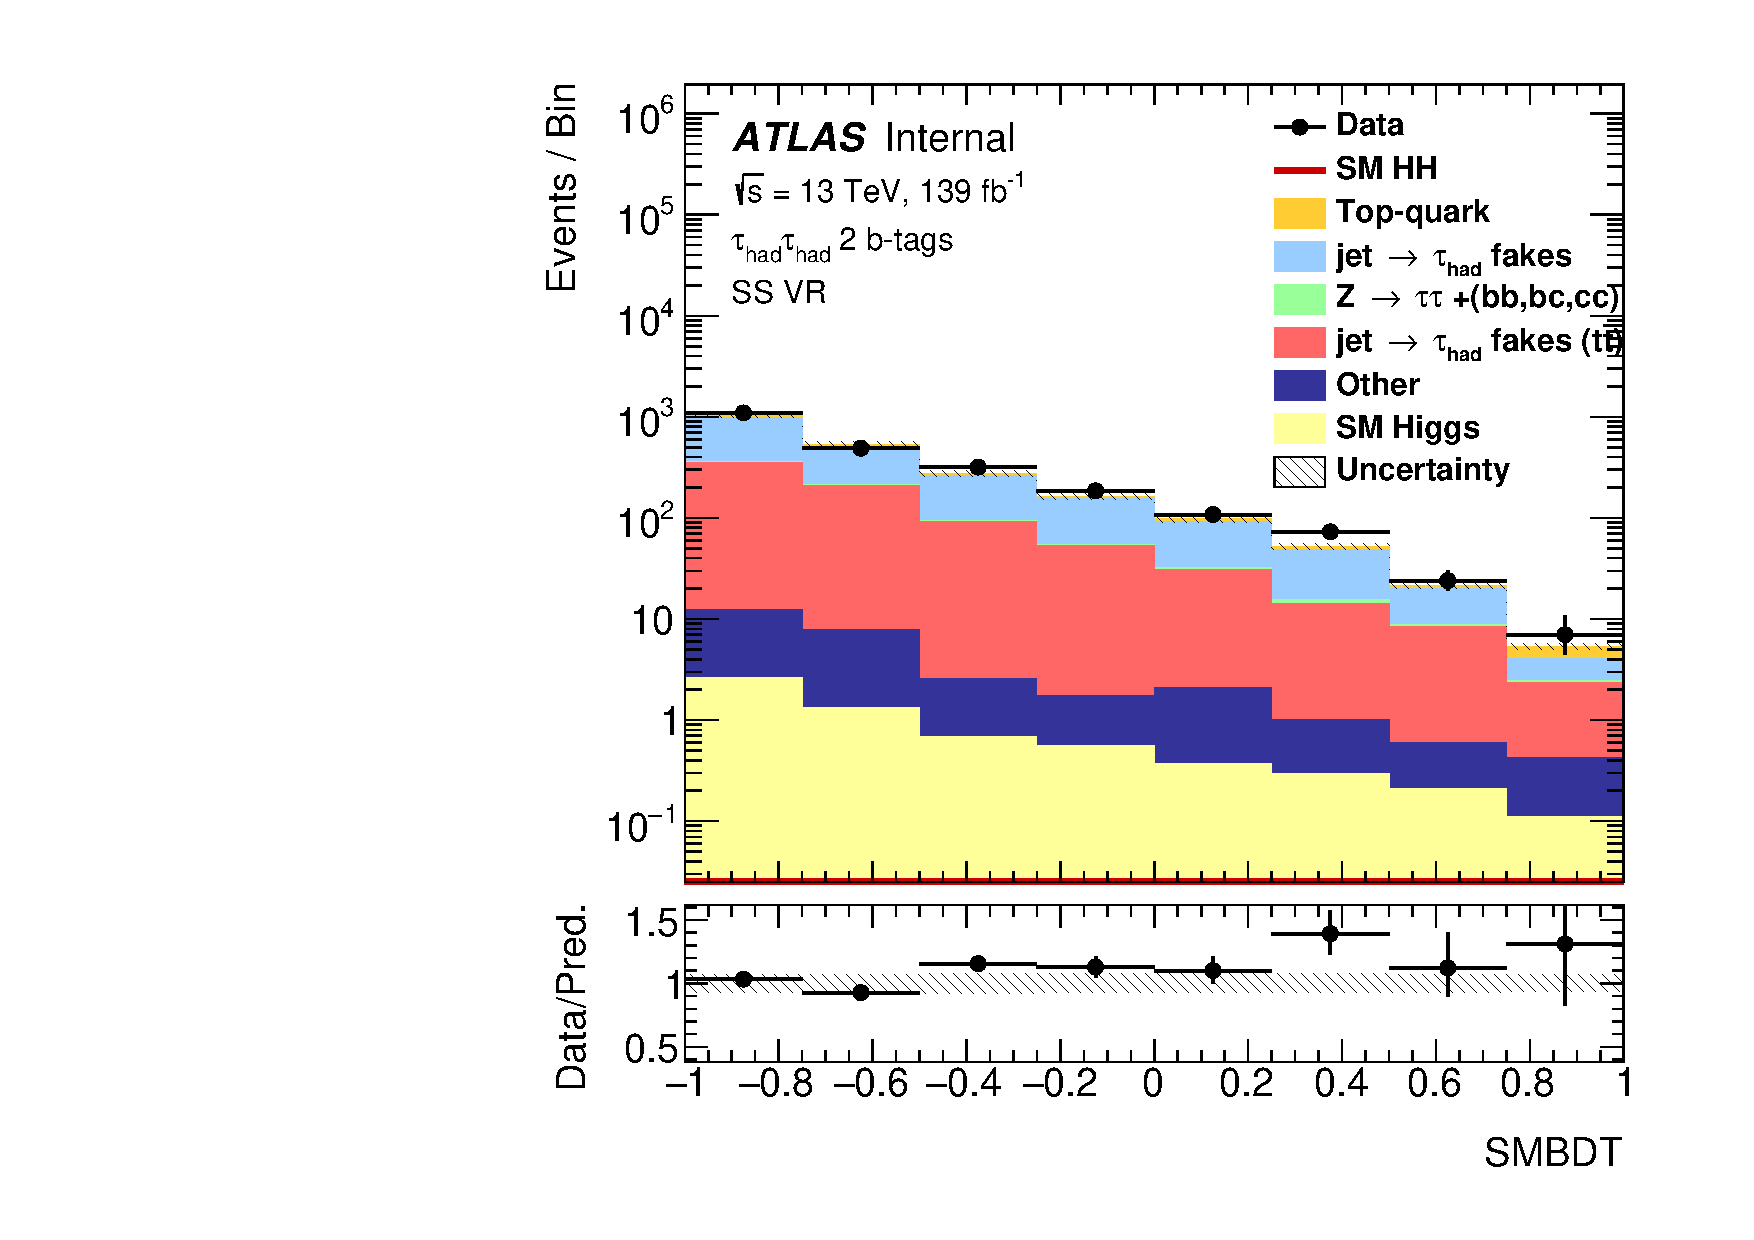
\includegraphics[width=.45\textwidth]{figures/mva/HH/HadHad/Region_BMin0_incJet1_distSMBDT_J2_Y2015_DLLSS_T2_SpcTauHH_L0_Prefitlog.pdf}
\caption{Pre-fit PNN score distributions for the $300, 500, 1000$ GeV mass points and pre-fit SM BDT distribution in the di-Higgs $bb\tau_{had}\tau_{had}$ same-sign validation region. The signal is normalised to the input cross section. (Inputs from 2020\textunderscore 11\textunderscore 26)}
\label{fig:HadHadPreselectionPNNScoreDistributionsSS}
\end{figure}

\Cref{tab:yields_LastMVABin_HadHad,tab:yields_LastMVABin_HadHad_PNN300,tab:yields_LastMVABin_HadHad_PNN500,tab:yields_LastMVABin_HadHad_PNN1000,tab:yields_LastMVABin_HadHad_PNN1600} 
show the event yields in the last 3 MVA bins of the signal region, which are the most significant bins
for the signal extraction. Additionally,
in~\Cref{tab:significance_smbdt_bins_HadHad} the signal over
background ratio and the signal significance is shown for all bins (as
they enter the final fit) of the SMBDT distribution.

\begin{table}
  \centering
  \begin{tabular}{lccc}
  \toprule
  Process & 3rd-to-last bin & 2nd-to-last bin & Last bin \\
  \midrule
  Diboson &	0.574	$\pm$ 0.186	& 0.405	$\pm$ 0.130	& 0.147	$\pm$ 0.076 \\
  Fake &	4.518	$\pm$ 1.352	& 1.664	$\pm$ 0.959	& 0.507	$\pm$ 0.438 \\
  VBFHtautau &	0.087	$\pm$ 0.014	& 0.047	$\pm$ 0.011	& 0.037	$\pm$ 0.009 \\
  WHbb &	0.004	$\pm$ 0.001	& 0.004	$\pm$ 0.001	& 0.003	$\pm$ 0.001 \\
  WHtautau &	0.038	$\pm$ 0.023	& 0.008	$\pm$ 0.008	& 0.000	$\pm$ 0.000 \\
  Wjets &	0.532	$\pm$ 0.335	& 0.559	$\pm$ 0.251	& 0.167	$\pm$ 0.167 \\
  ZHbb &	0.816	$\pm$ 0.022	& 0.411	$\pm$ 0.011	& 0.252	$\pm$ 0.055 \\
  ZHtautau &	1.043	$\pm$ 0.075	& 1.013	$\pm$ 0.073	& 0.599	$\pm$ 0.056 \\
  Zhf &		12.218	$\pm$ 1.352	& 6.593	$\pm$ 0.904	& 2.370	$\pm$ 0.415 \\
  Zlf &		1.155	$\pm$ 0.781	& 0.254	$\pm$ 0.103	& 0.069	$\pm$ 0.049 \\
  ggFHtautau &	0.973	$\pm$ 0.141	& 0.742	$\pm$ 0.128	& 0.483	$\pm$ 0.098 \\
  stop &	1.347	$\pm$ 0.458	& 0.533	$\pm$ 0.267	& 0.435	$\pm$ 0.230 \\
  ttH &		0.955	$\pm$ 0.042	& 0.712	$\pm$ 0.037	& 0.487	$\pm$ 0.031 \\
  ttW &		0.039	$\pm$ 0.014	& 0.031	$\pm$ 0.012	& 0.017	$\pm$ 0.008 \\
  ttZ &		0.265	$\pm$ 0.033	& 0.132	$\pm$ 0.021	& 0.061	$\pm$ 0.015 \\
  ttbar &	4.656	$\pm$ 0.851	& 2.955	$\pm$ 0.704	& 0.649	$\pm$ 0.335 \\
  ttbarFake &	4.500	$\pm$ 0.918	& 3.028	$\pm$ 0.703	& 0.330	$\pm$ 0.195 \\
  \midrule
  Total Bkg.\ & 33.721	$\pm$ 2.494	& 19.091 $\pm$ 1.707	& 6.611	$\pm$ 0.788 \\
  \midrule
  hhttbb ggF SM &	0.719	$\pm$ 0.007	& 0.935	$\pm$ 0.008	& 1.578	$\pm$ 0.011 \\
  hhttbb VBF SM &	0.019	$\pm$ 0.000	& 0.020	$\pm$ 0.000	& 0.023	$\pm$ 0.000 \\
  \bottomrule
\end{tabular}

  \caption{Pre-fit event yields in the last three BDT bins of the
    di-Higgs \hadhad channel (Inputs from 2021\textunderscore
    04\textunderscore 08). The uncertainty is stat-only.}
  \label{tab:yields_LastMVABin_HadHad}
\end{table}

\begin{table}
  \centering
  \begin{tabular}{lccc}
  \toprule
  Process & 3rd-to-last bin & 2nd-to-last bin & Last bin \\
  \midrule
  Diboson &	0.090	$\pm$ 0.070	& 0.031	$\pm$ 0.031	& 0.038	$\pm$ 0.038 \\
  Fake &	2.399	$\pm$ 1.725	& 3.906	$\pm$ 1.527	& 2.301	$\pm$ 1.234 \\
  VBFHtautau &	0.000	$\pm$ 0.000	& 0.000	$\pm$ 0.000	& 0.002	$\pm$ 0.002 \\
  WHbb &	0.004	$\pm$ 0.004	& 0.000	$\pm$ 0.000	& 0.000	$\pm$ 0.000 \\
  WHtautau &	0.005	$\pm$ 0.005	& 0.000	$\pm$ 0.000	& 0.000	$\pm$ 0.000 \\
  Wjets &	0.000	$\pm$ 0.000	& 0.000	$\pm$ 0.000	& 0.000	$\pm$ 0.000 \\
  ZHbb &	0.047	$\pm$ 0.008	& 0.018	$\pm$ 0.005	& 0.016	$\pm$ 0.004 \\
  ZHtautau &	0.030	$\pm$ 0.014	& 0.024	$\pm$ 0.011	& 0.028	$\pm$ 0.013 \\
  Zhf &		3.731	$\pm$ 1.390	& 1.125	$\pm$ 0.614	& 0.646	$\pm$ 0.354 \\
  Zlf &		0.264	$\pm$ 0.170	& 0.000	$\pm$ 0.000	& 0.032	$\pm$ 0.042 \\
  ggFHtautau &	0.065	$\pm$ 0.038	& 0.006	$\pm$ 0.006	& 0.058	$\pm$ 0.041 \\
  stop &	0.372	$\pm$ 0.336	& 0.635	$\pm$ 0.287	& 0.271	$\pm$ 0.192 \\
  ttH &		0.216	$\pm$ 0.020	& 0.153	$\pm$ 0.016	& 0.129	$\pm$ 0.015 \\
  ttW &		0.065	$\pm$ 0.022	& 0.026	$\pm$ 0.011	& 0.026	$\pm$ 0.009 \\
  ttZ &		0.060	$\pm$ 0.019	& 0.034	$\pm$ 0.014	& 0.035	$\pm$ 0.018 \\
  ttbar &	14.591	$\pm$ 1.562	& 8.734	$\pm$ 1.203	& 8.043	$\pm$ 1.159 \\
  ttbarFake &	16.932	$\pm$ 1.877	& 11.925	$\pm$ 1.542	& 7.479	$\pm$ 1.206 \\
  \midrule
  Total Bkg. &  38.870  $\pm$ 3.320	& 26.616 $\pm$ 2.572 & 19.105 $\pm$ 2.118 \\
  \midrule
  Hhhbbtautau300 &	7.008	$\pm$ 0.150	& 8.051	$\pm$ 0.161	& 10.933	$\pm$ 0.189 \\
  \bottomrule
\end{tabular}

  \caption{Pre-fit event yields in the last three PNN bins for X(300
    GeV) of the di-Higgs \hadhad channel (Inputs from
    2021\textunderscore 04\textunderscore 08). The uncertainty is stat-only.}
  \label{tab:yields_LastMVABin_HadHad_PNN300}
\end{table}

\begin{table}
  \centering
  \begin{tabular}{lccc}
  \toprule
  Process & 3rd-to-last bin & 2nd-to-last bin & Last bin \\
  \midrule
  Diboson &	1.102	$\pm$ 0.232	& 0.438	$\pm$ 0.174	& 0.198	$\pm$ 0.095 \\
  Fake &	7.166	$\pm$ 1.444	& 3.814	$\pm$ 1.072	& 0.090	$\pm$ 0.422 \\
  VBFHtautau &	0.045	$\pm$ 0.011	& 0.039	$\pm$ 0.009	& 0.024	$\pm$ 0.007 \\
  WHbb &	0.001	$\pm$ 0.001	& 0.002	$\pm$ 0.001	& 0.002	$\pm$ 0.001 \\
  WHtautau &	0.010	$\pm$ 0.010	& 0.013	$\pm$ 0.013	& 0.000	$\pm$ 0.000 \\
  Wjets &	0.385	$\pm$ 0.197	& 0.204	$\pm$ 0.148	& 0.305	$\pm$ 0.216 \\
  ZHbb &	0.657	$\pm$ 0.048	& 0.330	$\pm$ 0.019	& 0.185	$\pm$ 0.055 \\
  ZHtautau &	0.715	$\pm$ 0.061	& 0.749	$\pm$ 0.063	& 0.375	$\pm$ 0.044 \\
  Zhf &		19.294	$\pm$ 1.906	& 6.634	$\pm$ 1.078	& 2.923	$\pm$ 0.575 \\
  Zlf &		1.897	$\pm$ 0.753	& 0.506	$\pm$ 0.472	& 0.117	$\pm$ 0.126 \\
  ggFHtautau &	1.004	$\pm$ 0.146	& 0.432	$\pm$ 0.090	& 0.248	$\pm$ 0.076 \\
  stop &	1.439	$\pm$ 0.453	& 0.848	$\pm$ 0.440	& 0.426	$\pm$ 0.225 \\
  ttH &		0.853	$\pm$ 0.040	& 0.573	$\pm$ 0.033	& 0.418	$\pm$ 0.028 \\
  ttW &		0.060	$\pm$ 0.018	& 0.017	$\pm$ 0.009	& 0.012	$\pm$ 0.006 \\
  ttZ &		0.344	$\pm$ 0.039	& 0.159	$\pm$ 0.025	& 0.060	$\pm$ 0.015 \\
  ttbar &	4.693	$\pm$ 0.900	& 1.850	$\pm$ 0.572	& 0.155	$\pm$ 0.155 \\
  ttbarFake &	5.615	$\pm$ 1.008	& 1.735	$\pm$ 0.576	& 0.631	$\pm$ 0.293 \\
  \midrule
  Total Bkg. &  45.282	$\pm$ 2.905	& 18.341 $\pm$ 1.858	& 6.169	$\pm$ 0.868 \\
  \midrule
  Hhhbbtautau500 &	23.923	$\pm$ 0.466	& 41.670	$\pm$ 0.611	& 122.360	$\pm$ 1.047 \\
  \bottomrule
\end{tabular}

  \caption{Pre-fit event yields in the last three PNN bins for X(500
    GeV) of the di-Higgs \hadhad channel (Inputs from
    2021\textunderscore 04\textunderscore 08). The uncertainty is stat-only.}
  \label{tab:yields_LastMVABin_HadHad_PNN500}
\end{table}

\begin{table}
  \centering
  \begin{tabular}{lccc}
  \toprule
  Process & 3rd-to-last bin & 2nd-to-last bin & Last bin \\
  \midrule
  Diboson &	41.496	$\pm$ 1.583	& 2.131	$\pm$ 0.305	& 0.366	$\pm$ 0.137 \\
  Fake &	1352.019	$\pm$ 25.818	& 2.046	$\pm$ 0.730	& 0.596	$\pm$ 0.395 \\
  VBFHtautau &	1.470	$\pm$ 0.059	& 0.139	$\pm$ 0.018	& 0.032	$\pm$ 0.009 \\
  WHbb &	0.163	$\pm$ 0.018	& 0.001	$\pm$ 0.001	& 0.001	$\pm$ 0.001 \\
  WHtautau &	0.372	$\pm$ 0.060	& 0.013	$\pm$ 0.009	& 0.025	$\pm$ 0.018 \\
  Wjets &	52.594	$\pm$ 6.506	& 0.393	$\pm$ 0.188	& 0.146	$\pm$ 0.146 \\
  ZHbb &	13.746	$\pm$ 0.216	& 0.542	$\pm$ 0.010	& 0.336	$\pm$ 0.007 \\
  ZHtautau &	7.402	$\pm$ 0.196	& 0.334	$\pm$ 0.041	& 0.283	$\pm$ 0.039 \\
  Zhf &		1536.942	$\pm$ 21.267	& 23.735	$\pm$ 1.461	& 3.276	$\pm$ 0.422 \\
  Zlf &		107.213	$\pm$ 37.017	& 2.229	$\pm$ 0.431	& 0.150	$\pm$ 0.064 \\
  ggFHtautau &	12.683	$\pm$ 0.515	& 0.989	$\pm$ 0.147	& 0.382	$\pm$ 0.088 \\
  stop &	270.483	$\pm$ 6.586	& 1.606	$\pm$ 0.487	& 0.000	$\pm$ 0.000 \\
  ttH &		33.277	$\pm$ 0.243	& 1.229	$\pm$ 0.050	& 0.171	$\pm$ 0.019 \\
  ttW &		13.633	$\pm$ 0.297	& -0.034	$\pm$ 0.041	& 0.004	$\pm$ 0.004 \\
  ttZ &		31.801	$\pm$ 0.481	& 0.472	$\pm$ 0.042	& 0.074	$\pm$ 0.013 \\
  ttbar &	3579.542	$\pm$ 24.729	& 1.011	$\pm$ 0.461	& 0.135	$\pm$ 0.135 \\
  ttbarFake &	2491.067	$\pm$ 21.585	& 0.324	$\pm$ 0.195	& 0.000	$\pm$ 0.000 \\
  \midrule
  Total Bkg. &  9545.902	$\pm$ 60.461	& 37.162 $\pm$ 1.871	& 5.977	$\pm$ 0.638 \\
  \midrule
  Hhhbbtautau1000 &	11.068	$\pm$ 0.364	& 36.547	$\pm$ 0.663	& 389.654	$\pm$ 2.169 \\
  \bottomrule
\end{tabular}

  \caption{Pre-fit event yields in the last three PNN bins (only 3 bins in total) for X(1000 GeV) of the di-Higgs \hadhad channel (Inputs from
    2021\textunderscore 04\textunderscore 08). The uncertainty is stat-only.}
  \label{tab:yields_LastMVABin_HadHad_PNN1000}
\end{table}

\begin{table}
  \centering
  \begin{tabular}{lcc}
  \toprule
  Process & 2nd-to-last bin & Last bin \\
  \midrule
  Diboson	& 43.737	$\pm$ 1.615	& 0.256	$\pm$ 0.095 \\
  Fake		& 1354.209	$\pm$ 25.828	& 0.452	$\pm$ 0.359 \\
  VBFHtautau	& 1.597	$\pm$ 0.061	& 0.044	$\pm$ 0.010 \\
  WHbb		& 0.165	$\pm$ 0.018	& 0.000	$\pm$ 0.000 \\
  WHtautau	& 0.406	$\pm$ 0.063	& 0.004	$\pm$ 0.004 \\
  Wjets		& 53.033	$\pm$ 6.510	& 0.100	$\pm$ 0.090 \\
  ZHbb		& 14.582	$\pm$ 0.216	& 0.041	$\pm$ 0.003 \\
  ZHtautau	& 7.993	$\pm$ 0.204	& 0.026	$\pm$ 0.011 \\
  Zhf		& 1560.393	$\pm$ 21.317	& 3.562	$\pm$ 0.391 \\
  Zlf		& 109.045	$\pm$ 37.019	& 0.546	$\pm$ 0.151 \\
  ggFHtautau	& 13.757	$\pm$ 0.536	& 0.297	$\pm$ 0.085 \\
  stop		& 272.090	$\pm$ 6.604	& 0.000	$\pm$ 0.000 \\
  ttH		& 34.536	$\pm$ 0.249	& 0.141	$\pm$ 0.017 \\
  ttW		& 13.603	$\pm$ 0.300	& 0.000	$\pm$ 0.000 \\
  ttZ		& 32.251	$\pm$ 0.482	& 0.096	$\pm$ 0.025 \\
  ttbar		& 3580.259	$\pm$ 24.732	& 0.430	$\pm$ 0.304 \\
  ttbarFake	& 2491.392	$\pm$ 21.586	& 0.000	$\pm$ 0.000 \\
  \midrule
  Total Bkg.    & 9583.048	$\pm$ 60.489	& 5.997	$\pm$ 0.650 \\
  \midrule
  Hhhbbtautau1600	& 5.711	$\pm$ 0.365	& 145.895	$\pm$ 1.860 \\
  \bottomrule
\end{tabular}

  \caption{Pre-fit event yields in the last last two MVA bins (only 2 bins in total) for X(1600 GeV) of the di-Higgs \hadhad channel (Inputs from
    2021\textunderscore 04\textunderscore 08). The uncertainty is stat-only.}
  \label{tab:yields_LastMVABin_HadHad_PNN1600}
\end{table}

\begin{table}
  \centering
  {
    \footnotesize
    \begin{tabular}{lcccccc}
  \toprule
  & Bin 1 & Bin 2 & Bin 3 & Bin 4 & Bin 5 & Bin 6 \\
  \midrule
  Non-res.\ Sig. & 0.02 $\pm$ 0.00 & 0.04 $\pm$ 0.00 & 0.07 $\pm$ 0.00 & 0.12 $\pm$ 0.00 & 0.17 $\pm$ 0.00 & 0.21 $\pm$ 0.00 \\
  Total Bkg. & 5324.86 $\pm$ 47.14 & 1508.36 $\pm$ 19.63 & 946.19 $\pm$ 15.33 & 657.49 $\pm$ 23.81 & 359.59 $\pm$ 9.00 & 261.38 $\pm$ 7.50 \\
  $\text{S} / \text{B}$ & 0.000 & 0.000 & 0.000 & 0.000 & 0.000 & 0.001 \\
  $\text{S} / \sqrt{\text{B}}$ & 0.000 & 0.001 & 0.002 & 0.005 & 0.009 & 0.013 \\

  \midrule
  & Bin 7 & Bin 8 & Bin 9 & Bin 10 & Bin 11 & Bin 12 \\
  \midrule
  Non-res.\ Sig. & 0.26 $\pm$ 0.00 & 0.34 $\pm$ 0.00 & 0.44 $\pm$ 0.01 & 0.52 $\pm$ 0.01 & 0.72 $\pm$ 0.01 & 0.94 $\pm$ 0.01 \\
  Total Bkg. & 187.30 $\pm$ 6.31 & 133.56 $\pm$ 5.34 & 93.18 $\pm$ 4.87 & 57.72 $\pm$ 3.28 & 33.72 $\pm$ 2.49 & 19.09 $\pm$ 1.71 \\
  $\text{S} / \text{B}$ & 0.001   & 0.003   & 0.005   & 0.009   & 0.021   & 0.049 \\
  $\text{S} / \sqrt{\text{B}}$ & 0.019   & 0.029   & 0.045   & 0.068   & 0.124   & 0.214 \\

  \midrule
  & Bin 13 & & & & & \\
  \midrule
  Non-res.\ Sig. & 1.58 $\pm$ 0.01 &&&&&\\
  Total Bkg. & 6.61 $\pm$ 0.79 &&&&&\\
  $\text{S} / \text{B}$ & 0.239 &&&&&\\
  $\text{S} / \sqrt{\text{B}}$ &  0.614 &&&&&\\

  \bottomrule
\end{tabular}

  }
  \caption{Signal over background and signal significance for the SM
    non-resonant signal in bins of the final discriminant entering the
    fit of the di-Higgs \hadhad channel. All uncertainties are
    statistical only. (Inputs from 2021\textunderscore
    04\textunderscore 08).}
  \label{tab:significance_smbdt_bins_HadHad}
\end{table}

The hyperparameters for the MVAs were chosen based on a 5-fold cross
validation (CV) approach that is independently performed for the
training on even- and odd-numbered events. This is to ensure that the
data used to optimize the hyperparameters of the method (and training)
does not enter the final signal extraction fit, hence avoiding the
introduction of biases based on the optimization.

The values of the hyperparameters are chosen randomly from a
predefined grid of values
(c.f.~\Cref{tab:hadhad_mva_bdt_param_grid},\Cref{tab:hadhad_mva_pnn_param_grid}). A
total of 2000 realizations of random hyperparameters are checked. For
every realization, the 5-fold cross validation is performed for both
events with even and odd event numbers.

\begin{table}
  \centering
  \begin{tabular}{ll}
    \toprule
    Hyperparameter & Grid \\
    \midrule
    \texttt{NTrees} & 200, 400, 800, 1000, 1500, 2000 \\
    \texttt{MaxDepth} & 1, 2, 3 \\
    \texttt{MinNodeSize} & 5\%, 1\%, 0.1\%, 0.01\% \\
    \texttt{BoostType} & ``Grad'', ``AdaBoost''\\
    \texttt{Shrinkage} (for \texttt{BoostType} ``Grad'') & 0.01, 0.02, 0.04, 0.08, 0.1, 0.15, 0.2, 0.3, 0.4 \\
    \texttt{AdaBoostBeta} (for \texttt{BoostType} ``AdaBoost'') & 0.01, 0.02, 0.04, 0.08, 0.1, 0.15, 0.2, 0.3, 0.4 \\
    \texttt{IgnoreNegativeWeightsInTraining} & Yes, No \\
    \bottomrule
  \end{tabular}
  \caption{Grid of TMVA BDT hyperparameters chosen for the
    optimization in \hadhad. In addition to these parameters, various
    transformations of the input variables were tested in the
    optimization but did not show any significant difference compared
    to the untransformed input variables.}
  \label{tab:hadhad_mva_bdt_param_grid}
\end{table}


\begin{table}
  \centering
  \begin{tabular}{ll}
    \toprule
    Hyperparameter & Grid \\
    \midrule
    \texttt{Epochs} & 50, 100, 200, 400 \\
    \texttt{BatchSize} & 64, 128, 256 \\
    \texttt{LearningRate} & 0.01, 0.02, 0.05, 0.1, 0.2 \\
    \texttt{LearningRateDecay} & $10^{-6}$, $10^{-5}$, $10^{-4}$, $10^{-3}$ \\
    \texttt{NumberOfLayers} & 1, 2, 3, 4, 5 \\
    \texttt{LayerSize} (first layer) & 16, 32, 64, 128 \\
    \texttt{LayerSize} (intermediate layers) & 16, 32, 64, 128 \\
    \texttt{LayerSize} (last layer) & 16, 32, 64, 128 \\
    \bottomrule
  \end{tabular}
  \caption{Grid of PNN hyperparameters chosen for the optimization in
    \hadhad. For optimization of the binary cross-entropy loss,
    stochastic gradient descent (SGD) is used in all cases with a
    Nesterov momentum of 0.9.}
  \label{tab:hadhad_mva_pnn_param_grid}
\end{table}


The cross validation is performed as follows for the even events (odd
events are analogous):
\begin{itemize}
\item The even events are randomly split into five disjoint subsets
  (i.e.\ 5-fold CV)
\item A subset is selected as the validation set; the remaining four
  subsets are used as the training set
\item The training is performed on the training set and subsequently
  evaluated on the validation set
\item The performance metric (area under the receiver operating curve)
  is evaluated on the validation set
\item This process is repeated until every subset was used as the
  validation set.
\item The metric is averaged across all folds and the standard
  deviation is calculated to estimate the stability of the metric
\end{itemize}
This is then also performed separately for the odd-numbered events.

The final selection of hyperparameters is performed by ordering the CV
results by decreasing average performance seperately for the even- and
odd-numbered events. Realizations of hyperparameters that lead to
large fluctuations of the CV metric are removed. After considering the
best performing hyperparametersets that are still compatible within
the standard deviation of the metric, it was found that the best
parameters for both the even and odd event split share similar
configurations (only differing in hyperparameters that were not
found to affect the classification performance). Therefore, a common
configuration was chosen for the training on even and odd events.

After selecting the hyperparameters according to this approach, two
MVAs are retrained on the entirety of the even- / odd-numbered events
(i.e.\ without holding out a fifth of the data for validation). For
the final application, it is ensured that the BDT that was optimized
and trained on even (odd) events is only applied to odd (even) events.

The di-Higgs \hadhad channel MVA trainings parameters are given in
Table~\ref{app:tab:parameters_BDT_HadHad} for the non-resonant SM
BDT\footnote{The 5-fold CV estimates of the ROC-AUC for this
  configuration are \num{0.9803 +- 0.008} and \num{0.9787 +- 0.0012}
  for the even and odd dataset, respectively.} and in
Table~\ref{tab:parameters_PNN_HadHad} for the resonant PNN.

\begin{table}
\centering
\small
\begin{tabular}{|c|c|}
\hline
Parameter & Value\\
\hline
NTrees & 1500\\
MaxDepth & 2\\
MinNodeSize & 1\%\\
BoostType & Grad\\
Shrinkage & 0.2\\
IgnoreNegWeightsInTraining & True\\
\hline
\end{tabular}
\caption{Training parameters used for the di-Higgs \hadhad non-resonant BDT.}
\label{tab:parameters_BDT_HadHad}
\end{table}

\begin{table}
\centering
\small
\begin{tabular}{|c|c|}
\hline
Parameter & Value\\
\hline
Epochs & 200\\
Batch-size & 128\\
Learning rate & 0.2\\
Learning rate decay & 1e-5\\
Nesterov momentum & 0.9 \\
Layer sizes & 128 128 128 16\\
\hline
\end{tabular}
\caption{Training parameters used for the di-Higgs \hadhad resonant PNN.}
\label{tab:parameters_PNN_HadHad}
\end{table}

Studies on the performance of the MVAs are reported in Appendix~\ref{sec:appendix_pnn_HH}.


\subsection{$\tau_\mathrm{lep}\tau_\mathrm{had}$ channel}
\label{ssec:mva_lephad}

Variables used for the di-Higgs $bb\tau_\mathrm{lep}\tau_\mathrm{had}$ channels are given in Table~\ref{tab:lephadmvavars}. This choice of variables were taken from the previous iteration of the analysis, though the addition of the $p_\mathrm{T}^{\tau\tau}$, $p_\mathrm{T}^{bb}$, and $m_\mathrm{T}^2$ variables were considered, and shown to provide negligible improvement to the performance metric described below: $\lesssim 1\%$ in both the SLT and LTT channels. The chosen variables are described below:

\begin{itemize}
\item $m_{bb}$: The invariant mass of the di-$b$-jet system;
\item $m_{\tau\tau}^\mathrm{MMC}$: The invariant mass of the di-$\tau$ system, calculated using the MMC;
\item $m_{HH}$: The invariant mass of the di-Higgs system is reconstructed from the di-$\tau_{had}$ and di-$b$-jet 4-vectors;
\item $\Delta p_\mathrm{T}(\ell, \tau_\mathrm{had-vis})$; The difference between the transverse momentum of the lepton and hadronic $\tau$;
\item $\Delta  R(b, b)$: The  $\Delta R$ between the two $b$-jets.
\item $\Delta  R(\tau, \tau)$: The  $\Delta R$ between the visible-$\tau$ decay products;
\item $\Delta\phi(\tau^\tau, bb)$: The $\Delta\phi$ between the di-$\tau$ and di-$b$ systems;
\item Sub-leading $b$-jet $p_\mathrm{T}$: The transverse momentum of the sub-leading $b$-jet;
\item $E^\mathrm{miss}_\mathrm{T}$: The missing transverse momentum of the event, as described in section~\ref{subsec:met};
\item $m_\mathrm{T}^W$: The transverse mass between the lepton and the $E_\mathrm{T}^\mathrm{mass}$ is defined as:

$m_\mathrm{T}^W=\sqrt{2p_\mathrm{T}^\ell E_\mathrm{T}^\mathrm{miss}(1-\cos\Delta\phi)}$,

where $p_\mathrm{T}^\ell$ is the transverse momentum of the lepton. Signal events tend to have a lower $m_\mathrm{T}^W$ than the $t\bar t$ process because the transverse mass of a lepton and neutrino decaying from a $W$ boson in a $t\bar t$ event tends to peak at $m_W\approx 80~\mathrm{GeV}$;

\item $E^\mathrm{miss}_\mathrm{T}~\phi$ Centrality: The position in $\phi$ of $E_{T}^{\mathrm{miss}}$ between taus;
\item $\Delta\phi(\ell, E^\mathrm{miss}_\mathrm{T})$: The $\Delta\phi$ between the lepton and $E^\mathrm{miss}_\mathrm{T}$;
\item $H_\mathrm{T}$: The sum of hadronic transverse energy in the event, perpendicular to the beamline;
\item $\Delta\phi(\tau\tau, E^\mathrm{miss}_\mathrm{T})$: The $\Delta\phi$ between the di-$\tau$ system and $E^\mathrm{miss}_\mathrm{T}$.
\end{itemize}

\begin{table}
\caption{Features variables used for the di-Higgs $bb\tau_\mathrm{lep}\tau_\mathrm{had}$ SLT and LTT channels}
\label{tab:lephadmvavars}
  \centering
  \begin{tabular}{ccc}
    Variable                                           & SLT    & LTT    \\
    \hline
    $m_{bb}$                                           & {\color{green}\ding{51}} & {\color{green}\ding{51}} \\
    $m^\mathrm{MMC}_{\tau\tau}$                        & {\color{green}\ding{51}} & {\color{green}\ding{51}} \\
    $m_{HH}$                                           & {\color{green}\ding{51}} & {\color{green}\ding{51}} \\
    $\Delta R(\tau,\tau)$                              & {\color{green}\ding{51}} & {\color{green}\ding{51}} \\
    $\Delta p_\mathrm{T}(\ell, \tau_\mathrm{had-vis})$ & {\color{green}\ding{51}} & {\color{green}\ding{51}} \\
    $\Delta R(b,b)$                                    & {\color{green}\ding{51}} &                          \\
    $\Delta\phi(\tau^\tau, bb)$                        & {\color{green}\ding{51}} &                          \\
    Sub-leading $b$-jet $p_\mathrm{T}$                 & {\color{green}\ding{51}} &                          \\
    $m_\mathrm{T}^W$                                   & {\color{green}\ding{51}} &                          \\
    $E^\mathrm{miss}_\mathrm{T}$                       & {\color{green}\ding{51}} &                          \\
    $E^\mathrm{miss}_\mathrm{T}~\phi$ Centrality       & {\color{green}\ding{51}} &                          \\
    $\Delta\phi(\ell, E^\mathrm{miss}_\mathrm{T})$     &                          & {\color{green}\ding{51}} \\
    $H_\mathrm{T}$                                     &                          & {\color{green}\ding{51}} \\
    $\Delta\phi(\tau\tau, E^\mathrm{miss}_\mathrm{T})$ &                          & {\color{green}\ding{51}} \\
  \end{tabular}                                                                                              \\
\end{table}

The PNN is trained in the signal region, to separate the signals from the sum of all backgrounds weighted by their respective cross sections (all backgrounds are 
taken from the MC for the training). Separate training and testing samples split by even / odd event numbers are used. The hyperparameter optimisation is 
performed on the older version of inputs (the changes are minor and have been introduced from v0.35 to v0.4 of the note), and due to a bug in the MVA inputs for 
the training, the $t\bar t$ background was included twice and the $WW$ background was not present. The impact was checked against a random scan of 
hyperparameters using the new samples with no known bugs to estimate the scale of the impact of the bug, and the improvement from the bug fix was seen to be 
on the level of 3--4\% (1.1--1.6\%) in the SLT (LTT) analysis category, so the old optimisation was adopted due to time constraints.

The di-Higgs \lephad channel MVA trainings parameters are given in Table~\ref{tab:parameters_NN_LepHad} for the non-resonant SM NN and in Table~\ref{tab:parameters_PNN_LepHad} for the resonant PNN.

\begin{table}
  \centering
  \small
  \begin{tabular}{|c|c|c|}
    \hline
    Parameter & Value for SLT & Value for LTT\\
    \hline
    Layer sizes & 512 512 & 512 512 512\\
    Epochs & 241 & 238\\
    Batch-size & 34 & 35\\
    Learning rate & 0.500 & 0.500\\
    Learning rate decay & 4.15$\times 10^{-3}$ & 4.20$\times 10^{-3}$\\
    Nesterov momentum & 0.944 & 0.791\\
    L2 regularisation weight & 1.00$\times 10^{-5}$ & 1.65$\times 10^{-5}$\\
    \hline
  \end{tabular}
  \caption{Training parameters used for the di-Higgs \lephad non-resonant NNs.}
  \label{tab:parameters_NN_LepHad}
\end{table}

\begin{table}
  \centering
  \small
  \begin{tabular}{|c|c|c|}
    \hline
    Parameter & Value for SLT & Value for LTT\\
    \hline
    Layer sizes & 512 512 & 256 256 256\\
    Epochs & 245 & 296\\
    Batch-size & 33 & 24\\
    Learning rate & 0.500 & 0.377\\
    Learning rate decay & 4.55$\times 10^{-3}$ & 3.38$\times 10^{-3}$\\
    Nesterov momentum & 0.975 & 0.975\\
    L2 regularisation weight & 5.45$\times 10^{-7}$ & 8.64$\times 10^{-6}$\\
    \hline
  \end{tabular}
  \caption{Training parameters used for the di-Higgs \lephad resonant PNNs.}
  \label{tab:parameters_PNN_LepHad}
\end{table}


These hyperparameters were chosen based on a machine learning approach which used Gaussian Process Regression. To compare these NNs the quadrature sum of approximated significances of bins containing at least 5 expected background events were compared, and to compare these PNNs the approximated significance after optimal (meaning a cut which maximises the approximated significance metric, with at least 5 expected background events passing the cut) single cuts on the output variables were compared. In the case of the PNNs the signal masses were averaged by weighting by the mass space nearest the chosen sample, to represent all parts of the mass space equally.

The metric is evaluated on a validation+testing sample (sample not used for training and used for validation and fitting) and the hyperparameters giving the best 
value of the metric on this sample are chosen. If this network was then used in the analysis, there would be a possible bias from the overlapping training and testing sets.
However, as described above, the networks are retrained after the hyperparameter optimisation using a slightly different dataset.
Possibly for this reason, the networks have a different set of weights and biases from the original training, meaning that the optimisation procedure has not resulted in the same solution, mitigating the possibility of this bias.
There is also pseudo-randomness in the network training procedure which results in the trained network having multiple possible sets of network weights and biases even without a change in the input dataset. The weights and biases of these MVAs have also been explicitly compared between the first training which occurred during hyperparameter optimisation, and the second training which is used in the analysis, and they can be seen to have changed.

Despite the above reasoning making it unlikely that any bias can result from the overlapping training and testing sets, this is tested explicitly as described below.
A nested cross-validation was also considered to ensure that there was no bias from the overlapping validation and 
testing datasets, however, the large $\tau_\text{lep}\tau_\text{had}$ samples sizes mean that this would have compromised the number of hyperparameter sets 
which could be trialled, and multiple MVAs would have been needed for each analysis category. In order to check that this approach did not introduce a significant 
bias, the full nested optimisation was performed in the non-resonant LTT search category, and the stat-only limits with no data-driven fakes were compared. The 
limit was found to deteriorate by just 0.6\% (1.7\%) with(out) retraining on the whole inner-fold from the nested cross validation. Similar studies were also performed 
in the non-resonant $\tau_\text{had}\tau_\text{had}$ category, and the differences in the estimated significance (as per the optimisation metric) was found to be on 
the level of 2.4\%.

Dropout regularisation was also tried, but were found to provide no improvements. The lower mass samples, where the $bb\tau_\mathrm{lep}\tau_\mathrm{had}$ 
channels are expected to provide most sensitivity, were given increased weights to see if this improved performance for these signal hypotheses, but no gains were 
observed, so this was not adopted.

Studies on the performance of the MVAs are reported in Appendix~\ref{sec:appendix_pnn_HH}.

Table~\ref{tab:yields_LastMVABin_LepHad_SLT},~\ref{tab:yields_LastMVABin_LepHad_LTT} shows the event yields in the last three MVA bin of the SLT, LTT signal region respectively,
 which are the most significant bins for the signal extraction. Additionally,
in~\Cref{tab:significance_smbdt_bins_LepHad} the signal over
background ratio and the signal significance is shown for all bins (as
they enter the final fit) of the SMBDT distribution.

\begin{table}
  \centering
  \footnotesize
  \begin{tabular}{|c|c|c|c|c|}
  \hline
  \multicolumn{5}{|c|}{Last bin}\\
  \hline
  Process & Last bin SM & Last bin 300 GeV & Last bin 500 GeV & Last bin 1000 GeV\\
  \hline
  ttbar &  $0.46 \pm 0.22$ &  $30.9 \pm 2$ &  $1.3 \pm 0.4$ &  $0.68 \pm 0.28$ \\
  Fake &  $1.2 \pm 0.7$ &  $16.7 \pm 2.4$ &  $1.1 \pm 0.6$ &  $0.8 \pm 0.6$ \\
  Stop &  $0.93 \pm 0.35$ &  $3 \pm 0.6$ &  $0.96 \pm 0.35$ &  $0.9 \pm 0.34$ \\
  ZHF &  $1.32 \pm 0.26$ &  $8.6 \pm 3.2$ &  $1.36 \pm 0.28$ &  $1.94 \pm 0.25$ \\
  ZLF &  $0.04 \pm 0.025$ &  $-0.25 \pm 0.25$ &  $0.029 \pm 0.029$ &  $0.27 \pm 0.18$ \\
  WHbb &  $0.0005 \pm 0.00035$ & 0 &  $0.0021 \pm 0.0012$ &  $0.0033 \pm 0.0013$ \\
  WHtautau & 0 & 0 &  $0.006 \pm 0.006$ & 0 \\
  qqZHbb &  $0.278 \pm 0.006$ &  $0.048 \pm 0.008$ &  $0.078 \pm 0.004$ &  $0.393 \pm 0.007$ \\
  ggZHbb &  $0.054 \pm 0.004$ &  $0.0008 \pm 0.0005$ &  $0.09 \pm 0.05$ &  $0.0342 \pm 0.0034$ \\
  qqZHtautau &  $0.28 \pm 0.04$ &  $0.059 \pm 0.016$ &  $0.084 \pm 0.023$ &  $0.158 \pm 0.028$ \\
  ggZHtautau &  $0.052 \pm 0.014$ &  $0.00016 \pm 0.00016$ &  $0.061 \pm 0.015$ &  $0.032 \pm 0.011$ \\
  ggFHtautau &  $0.25 \pm 0.05$ & 0 &  $0.111 \pm 0.034$ &  $0.15 \pm 0.04$ \\
  VBFHtautau &  $0.0047 \pm 0.0028$ &  $0.0025 \pm 0.0019$ &  $0.0018 \pm 0.0018$ &  $0.011 \pm 0.004$ \\
  ttH &  $0.221 \pm 0.019$ &  $0.09 \pm 0.012$ &  $0.166 \pm 0.016$ &  $0.082 \pm 0.012$ \\
  Wjets & 0 & 0 & 0 & 0 \\
  Diboson &  $0.2 \pm 0.09$ &  $0.24 \pm 0.09$ &  $0.15 \pm 0.09$ &  $0.53 \pm 0.13$ \\
  DY & 0 & 0 & 0 & 0 \\
   \hline 
  signal ggF &  $0.764 \pm 0.007$ &  $8.03 \pm 0.19$ &  $61.2 \pm 0.8$ &  $342.5 \pm 2.1$ \\
  signal VBF &  $0.00743 \pm 0.00024$  & NA  & NA  & NA  \\  
  \hline
  \multicolumn{5}{|c|}{Second-to-last bin}\\
  \hline
  Process & Last-1 bin SM & Last-1 bin 300 GeV & Last-1 bin 500 GeV & Last-1 bin 1000 GeV\\
    \hline
    ttbar &  $4.5 \pm 0.8$ &  $61.4 \pm 2.9$ &  $3.1 \pm 0.6$ &  $0.82 \pm 0.34$ \\
    Fake &  $1.9 \pm 0.8$ &  $25.4 \pm 3.2$ &  $0.8 \pm 0.6$ &  $1.4 \pm 0.8$ \\
    Stop &  $2.4 \pm 0.6$ &  $3 \pm 0.6$ &  $1.3 \pm 0.4$ &  $1.05 \pm 0.34$ \\
    ZHF &  $4 \pm 0.6$ &  $13 \pm 4$ &  $1.44 \pm 0.33$ &  $2.64 \pm 0.32$ \\
    ZLF &  $0.3 \pm 0.12$ &  $0.29 \pm 0.27$ &  $0.11 \pm 0.08$ &  $-0.03 \pm 0.08$ \\
    WHbb &  $0.0044 \pm 0.0015$ & 0 &  $0.0026 \pm 0.0015$ &  $0.0029 \pm 0.001$ \\
    WHtautau &  $0.013 \pm 0.009$ & 0 & 0 & 0 \\
    qqZHbb &  $0.448 \pm 0.008$ &  $0.086 \pm 0.01$ &  $0.075 \pm 0.004$ &  $0.232 \pm 0.005$ \\
    ggZHbb &  $0.16 \pm 0.05$ &  $0.0022 \pm 0.0008$ &  $0.0331 \pm 0.0034$ &  $0.06 \pm 0.04$ \\
    qqZHtautau &  $0.44 \pm 0.05$ &  $0.07 \pm 0.018$ &  $0.099 \pm 0.021$ &  $0.14 \pm 0.026$ \\
    ggZHtautau &  $0.126 \pm 0.022$ & 0 &  $0.059 \pm 0.015$ &  $0.017 \pm 0.008$ \\
    ggFHtautau &  $0.25 \pm 0.05$ &  $0.069 \pm 0.029$ &  $0.093 \pm 0.034$ &  $0.17 \pm 0.04$ \\
    VBFHtautau &  $0.012 \pm 0.005$ &  $0.009 \pm 0.004$ &  $0.0031 \pm 0.0022$ &  $0.01 \pm 0.004$ \\
    ttH &  $0.27 \pm 0.021$ &  $0.11 \pm 0.012$ &  $0.128 \pm 0.014$ &  $0.07 \pm 0.01$ \\
    Wjets & 0 & 0 & 0 & 0 \\
    Diboson &  $0.56 \pm 0.17$ &  $0.55 \pm 0.2$ &  $0.12 \pm 0.07$ &  $0.82 \pm 0.18$ \\
    DY & 0 & 0 & 0 & 0 \\
    \hline 
    signal ggF &  $0.599 \pm 0.006$ &  $7.53 \pm 0.18$ &  $21 \pm 0.5$ &  $42 \pm 0.7$ \\
    signal VBF &  $0.00869 \pm 0.00027$ & NA  & NA  & NA  \\    
    \hline
    \multicolumn{5}{|c|}{Third-to-last bin}\\
    \hline
    Process & Last-2 bin SM & Last-2 bin 300 GeV & Last-2 bin 500 GeV & Last-2 bin 1000 GeV\\
    \hline
    ttbar &  $9.1 \pm 1.1$ &  $88 \pm 3.4$ &  $5.2 \pm 0.9$ &  $209 \pm 5$ \\ 
    Fake &  $4.7 \pm 1.5$ &  $44 \pm 4$ &  $3.6 \pm 1.2$ &  $395 \pm 13$ \\ 
    Stop &  $5.3 \pm 0.8$ &  $4.3 \pm 0.7$ &  $1.2 \pm 0.4$ &  $104 \pm 4$ \\ 
    ZHF &  $7.1 \pm 0.7$ &  $11 \pm 4$ &  $3.3 \pm 0.7$ &  $212 \pm 6$ \\ 
    ZLF &  $0.54 \pm 0.28$ &  $0.9 \pm 0.7$ &  $0.04 \pm 0.11$ &  $21.9 \pm 2.9$ \\ 
    WHbb &  $0.021 \pm 0.004$ &  $0.013 \pm 0.008$ &  $0.0053 \pm 0.002$ &  $0.511 \pm 0.018$ \\ 
    WHtautau & 0 & 0 &  $0.005 \pm 0.005$ &  $0.101 \pm 0.029$ \\ 
    qqZHbb &  $0.677 \pm 0.011$ &  $0.123 \pm 0.012$ &  $0.121 \pm 0.006$ &  $3.355 \pm 0.022$ \\ 
    ggZHbb &  $0.24 \pm 0.06$ &  $0.0024 \pm 0.0009$ &  $0.043 \pm 0.004$ &  $1.31 \pm 0.11$ \\ 
    qqZHtautau &  $0.45 \pm 0.05$ &  $0.063 \pm 0.018$ &  $0.159 \pm 0.028$ &  $1.71 \pm 0.09$ \\ 
    ggZHtautau &  $0.161 \pm 0.024$ & 0 &  $0.059 \pm 0.015$ &  $0.57 \pm 0.05$ \\ 
    ggFHtautau &  $0.41 \pm 0.07$ &  $0.089 \pm 0.033$ &  $0.092 \pm 0.031$ &  $4.23 \pm 0.22$ \\ 
    VBFHtautau &  $0.033 \pm 0.008$ &  $0.009 \pm 0.004$ &  $0.01 \pm 0.004$ &  $0.402 \pm 0.026$ \\ 
    ttH &  $0.482 \pm 0.028$ &  $0.159 \pm 0.015$ &  $0.188 \pm 0.017$ &  $4.45 \pm 0.08$ \\ 
    Wjets &  $0.08 \pm 0.08$ &  $0.07 \pm 0.07$ & 0 &  $6 \pm 0.9$ \\ 
    Diboson &  $1.03 \pm 0.19$ &  $0.95 \pm 0.22$ &  $0.26 \pm 0.08$ &  $22.2 \pm 1.5$ \\ 
    DY & 0 & 0 & 0 &  $0.7 \pm 0.4$ \\ 
    \hline  
    signal ggF &  $0.596 \pm 0.006$ &  $7.36 \pm 0.18$ &  $20.6 \pm 0.5$ &  $40.5 \pm 0.7$ \\ 
    signal VBF &  $0.00997 \pm 0.00029$  & NA  & NA  & NA  \\ 
    \hline
  \end{tabular}
  \caption{Pre-fit event yields in the last, second-to-last and
  third-to-last MVA bin of the di-Higgs \lephad SLT channel (Inputs from 2021\textunderscore 07\textunderscore 04).}
  \label{tab:yields_LastMVABin_LepHad_SLT}
  \end{table}
 



\begin{table}
  \centering
  \footnotesize
  \begin{tabular}{|c|c|c|c|c|}
  \hline
  \multicolumn{5}{|c|}{Last bin}\\
  \hline
  Process & Last bin SM & Last bin 300 GeV & Last bin 500 GeV & Last bin 1000 GeV\\
  \hline
  ttbar &  $0.76 \pm 0.31$ &  $5 \pm 0.8$ &  $2.3 \pm 0.6$ &  $0.57 \pm 0.29$  \\
  Fake &  $2.6 \pm 1.4$ &  $3.7 \pm 1.7$ &  $1 \pm 0.8$ &  $0.9 \pm 0.9$  \\
  Stop &  $0.32 \pm 0.19$ &  $0.14 \pm 0.14$ &  $0.17 \pm 0.12$ &  $0.47 \pm 0.25$  \\
  ZHF &  $1.03 \pm 0.23$ &  $3.3 \pm 2.2$ &  $1.3 \pm 0.4$ &  $2.1 \pm 0.5$  \\
  ZLF &  $0.07 \pm 0.07$ & 0 &  $0.05 \pm 0.09$ &  $0.52 \pm 0.24$  \\
  WHbb &  $0.0013 \pm 0.0009$ & 0 & 0 &  $0.004 \pm 0.004$  \\
  WHtautau & 0 & 0 & 0 & 0  \\
  qqZHbb &  $0.0656 \pm 0.0032$ &  $0.0073 \pm 0.0028$ &  $0.0416 \pm 0.0027$ &  $0.0785 \pm 0.0032$  \\
  ggZHbb &  $0.0191 \pm 0.0026$ &  $0.0004 \pm 0.0004$ &  $0.0182 \pm 0.0024$ &  $0.0063 \pm 0.0014$  \\
  qqZHtautau &  $0.065 \pm 0.018$ &  $0.019 \pm 0.01$ &  $0.051 \pm 0.016$ &  $0.052 \pm 0.018$  \\
  ggZHtautau &  $0.02 \pm 0.009$ & 0 &  $0.022 \pm 0.009$ & 0  \\
  ggFHtautau &  $0.076 \pm 0.034$ & 0 &  $0.076 \pm 0.03$ &  $0.11 \pm 0.04$  \\
  VBFHtautau &  $0.005 \pm 0.0029$ & 0 &  $0.0018 \pm 0.0018$ &  $0.0035 \pm 0.0025$  \\
  ttH &  $0.044 \pm 0.008$ &  $0.014 \pm 0.005$ &  $0.065 \pm 0.01$ &  $0.031 \pm 0.007$  \\
  Wjets & 0 & 0 & 0 & 0  \\
  Diboson &  $-0.01 \pm 0.05$ &  $-0.05 \pm 0.04$ &  $0.03 \pm 0.04$ &  $0.44 \pm 0.14$  \\
  DY & 0 & 0 & 0 & 0  \\
  \hline   
 signal ggF &  $0.1977 \pm 0.0035$ &  $2.61 \pm 0.11$ &  $20.8 \pm 0.5$ &  $45.1 \pm 0.8$  \\
 signal VBF &  $0.00344 \pm 0.00017$ & NA  & NA  & NA  \\
  \hline
  \multicolumn{5}{|c|}{Second-to-last bin}\\
  \hline
  Process & Last-1 bin SM & Last-1 bin 300 GeV & Last-1 bin 500 GeV & Last-1 bin 1000 GeV\\
    \hline
    ttbar &  $3.8 \pm 0.7$ &  $8.5 \pm 1.1$ &  $2.5 \pm 0.6$ &  $108 \pm 4$ \\
    Fake &  $2 \pm 1.4$ &  $1.4 \pm 1.1$ &  $1.7 \pm 1.2$ &  $84 \pm 9$ \\
    Stop &  $0.37 \pm 0.21$ &  $0.45 \pm 0.24$ &  $0.08 \pm 0.08$ &  $18 \pm 1.7$ \\
    ZHF &  $1.6 \pm 0.4$ &  $2.5 \pm 1.1$ &  $0.82 \pm 0.19$ &  $86.4 \pm 3.4$ \\
    ZLF &  $0.15 \pm 0.1$ &  $0.07 \pm 0.07$ & 0 &  $11 \pm 4$ \\
    WHbb & 0 &  $0.0027 \pm 0.0027$ &  $0.0016 \pm 0.0011$ &  $0.0074 \pm 0.002$ \\
    WHtautau & 0 & 0 & 0 &  $0.047 \pm 0.021$ \\
    qqZHbb &  $0.083 \pm 0.004$ &  $0.022 \pm 0.005$ &  $0.0384 \pm 0.0033$ &  $0.826 \pm 0.013$ \\
    ggZHbb &  $0.0262 \pm 0.0029$ &  $0.00022 \pm 0.00016$ &  $0.0154 \pm 0.0023$ &  $0.44 \pm 0.06$ \\
    qqZHtautau &  $0.088 \pm 0.021$ &  $0.011 \pm 0.008$ &  $0.06 \pm 0.018$ &  $0.57 \pm 0.05$ \\
    ggZHtautau &  $0.027 \pm 0.01$ & 0 &  $0.028 \pm 0.01$ &  $0.212 \pm 0.028$ \\
    ggFHtautau &  $0.094 \pm 0.032$ &  $0.015 \pm 0.011$ &  $0.022 \pm 0.015$ &  $1.48 \pm 0.14$ \\
    VBFHtautau &  $0.005 \pm 0.0029$ &  $0.0025 \pm 0.0024$ &  $0.0043 \pm 0.0027$ &  $0.12 \pm 0.014$ \\
    ttH &  $0.062 \pm 0.01$ &  $0.02 \pm 0.005$ &  $0.046 \pm 0.009$ &  $1.45 \pm 0.05$ \\
    Wjets & 0 & 0 & 0 &  $0.83 \pm 0.31$ \\
    Diboson &  $0.14 \pm 0.08$ &  $0.1 \pm 0.09$ &  $0 \pm 0.04$ &  $3.7 \pm 0.4$ \\
    DY & 0 & 0 &  $0.15 \pm 0.15$ &  $0.15 \pm 0.15$ \\
     \hline 
    signal ggF&  $0.1402 \pm 0.0028$ &  $2.72 \pm 0.11$ &  $5.87 \pm 0.25$ &  $2.28 \pm 0.17$ \\
    signal VBF&  $0.00294 \pm 0.00016$ & NA  & NA  & NA  \\
    \hline
    \multicolumn{5}{|c|}{Third-to-last bin}\\
    \hline
    Process & Last-2 bin SM & Last-2 bin 300 GeV & Last-2 bin 500 GeV & Last-2 bin 1000 GeV\\
    \hline
    ttbar &  $6.3 \pm 0.9$ &  $9.7 \pm 1.2$ &  $3.4 \pm 0.7$ &  $4104 \pm 24$ \\
    Fake &  $1.4 \pm 1.3$ &  $6.6 \pm 2.4$ &  $2.4 \pm 1.3$ &  $2060 \pm 40$ \\
    Stop &  $0.85 \pm 0.34$ &  $0.3 \pm 0.21$ &  $0.47 \pm 0.25$ &  $179 \pm 5$ \\
    ZHF &  $4.8 \pm 0.9$ &  $2.6 \pm 1.1$ &  $2.1 \pm 0.4$ &  $368 \pm 14$ \\
    ZLF &  $0.18 \pm 0.09$ &  $0.25 \pm 0.2$ &  $0.05 \pm 0.04$ &  $37 \pm 9$ \\
    WHbb &  $0.0012 \pm 0.0008$ & 0 &  $0.001 \pm 0.0007$ &  $0.162 \pm 0.026$ \\
    WHtautau & 0 &  $0.006 \pm 0.006$ & 0 &  $0.131 \pm 0.033$ \\
    qqZHbb &  $0.124 \pm 0.006$ &  $0.041 \pm 0.007$ &  $0.0457 \pm 0.0032$ &  $2.95 \pm 0.05$ \\
    ggZHbb &  $0.0323 \pm 0.0032$ &  $0.0013 \pm 0.0006$ &  $0.0221 \pm 0.0026$ &  $1.01 \pm 0.13$ \\
    qqZHtautau &  $0.129 \pm 0.026$ &  $0.015 \pm 0.009$ &  $0.052 \pm 0.016$ &  $1.56 \pm 0.09$ \\
    ggZHtautau &  $0.039 \pm 0.012$ &  $0.004 \pm 0.004$ &  $0.028 \pm 0.01$ &  $0.53 \pm 0.04$ \\
    ggFHtautau &  $0.098 \pm 0.029$ &  $0.005 \pm 0.005$ &  $0.085 \pm 0.035$ &  $2.98 \pm 0.2$ \\
    VBFHtautau &  $0.014 \pm 0.005$ &  $0.0019 \pm 0.0019$ &  $0.0033 \pm 0.0023$ &  $0.248 \pm 0.02$ \\
    ttH &  $0.111 \pm 0.013$ &  $0.024 \pm 0.006$ &  $0.043 \pm 0.008$ &  $9.52 \pm 0.11$ \\
    Wjets & 0 & 0 & 0 &  $3.2 \pm 1$ \\
    Diboson &  $0.18 \pm 0.08$ &  $0 \pm 0.08$ &  $0.09 \pm 0.07$ &  $16.3 \pm 1$ \\
    DY & 0 & 0 & 0 &  $0.68 \pm 0.29$ \\
     \hline 
    signal ggF &  $0.1382 \pm 0.0028$ &  $2.61 \pm 0.11$ &  $4.93 \pm 0.23$ &  $0.009 \pm 0.009$ \\
    signal VBF &  $0.00331 \pm 0.00017$  & NA  & NA  & NA  \\    
    \hline
  \end{tabular}
  \caption{Pre-fit event yields in the last, second-to-last and
  third-to-last MVA bin of the di-Higgs \lephad LTT channel (Inputs from 2021\textunderscore 07\textunderscore 04).}
  \label{tab:yields_LastMVABin_LepHad_LTT}
  \end{table}
   
  
\begin{table}
  \centering
  {
    \footnotesize
    \begin{tabular}{lcccccccc}
  \toprule
  \multicolumn{9}{c}{SLT} \\
    \midrule
  & Bin 1 & Bin 2 & Bin 3 & Bin 4 & Bin 5 & Bin 6   & Bin 7 & Bin 8\\
  \midrule
  Non-res.\ Sig. & 0.0006 & 0.0027 & 0.0117 & 0.0548 & 0.1844 & 0.3819 & 0.4995 & 0.5515\\
  Total Bkg. & 12364 & 24839 & 20519 & 19074 & 14286 & 7236 & 3053 & 1285 \\
  $\text{S} / \text{B}$ & 0.000 & 0.000 & 0.000 & 0.000 & 0.000 & 0.0001 & 0.0002   & 0.0004 \\
  $\text{S} / \sqrt{\text{B}}$ & 0.000 & 0.000 & 0.0001 & 0.0004 & 0.0015 & 0.0045 & 0.009   & 0.0154 \\

  \midrule
 & Bin 9 & Bin 10 & Bin 11 & Bin 12 & Bin 13 & Bin 14 & Bin 15&   \\
  \midrule
  Non-res.\ Sig. &  0.5687 & 0.5769 & 0.569 & 0.5812 & 0.5922 &0.5946&0.6979& \\
  Total Bkg.  & 581 & 260 & 123 & 66.4  & 26.4 &13.1&4.84& \\
  $\text{S} / \text{B}$   & 0.001   & 0.0022   & 0.0046   & 0.0088 & 0.0224& 0.0456& 0.1443&\\
  $\text{S} / \sqrt{\text{B}}$   & 0.0236   & 0.0358   & 0.0512   & 0.0713 &  0.1152 &0.1646&0.3173&\\


  \midrule
    \multicolumn{9}{c}{LTT} \\
    \midrule
  & Bin 1 & Bin 2 & Bin 3 & Bin 4 & Bin 5 & Bin 6   & Bin 7 & Bin 8\\
  \midrule
  Non-res.\ Sig. & 0.0002 & 0.0018 & 0.0085 & 0.0202& 0.0514 & 0.0816 & 0.1078 & 0.1234\\
  Total Bkg. & 804 & 1421 & 1372 & 1207 & 904 & 606 & 342 & 182 \\
  $\text{S} / \text{B}$ & 0.000 & 0.000 & 0.000 & 0.000 & 0.0001 & 0.0001 & 0.0003   & 0.0007 \\
  $\text{S} / \sqrt{\text{B}}$ & 0.000 & 0.000 & 0.0002 & 0.0006 & 0.0017 & 0.0033 & 0.0058   & 0.0091 \\
  
    \midrule
 & Bin 9 & Bin 10 & Bin 11 & Bin 12 & Bin 13 & Bin 14 & Bin 15&   \\
  \midrule
  Non-res.\ Sig. &  0.131 & 0.1347 & 0.1375 & 0.142 & 0.1382 &0.1432&0.1947& \\
  Total Bkg.  & 111 & 66.5 & 38.0 & 30.3  & 14.3 &8.53&4.94& \\
  $\text{S} / \text{B}$   & 0.0012   & 0.002   & 0.0036   & 0.0047 & 0.0097& 0.0168& 0.0365&\\
  $\text{S} / \sqrt{\text{B}}$   & 0.0124   & 0.0165   & 0.0223   & 0.0258 &  0.0365 &0.049&0.0876&\\
  
  \bottomrule
\end{tabular}

  }
  \caption{Signal over background and signal significance for the SM
    non-resonant signal in bins of the final discriminant entering the
    fit of the di-Higgs \lephad channel. All uncertainties are
    statistical only. }
  \label{tab:significance_smbdt_bins_LepHad}
\end{table}


\cref{fig:lephadmvainputsslt,fig:lephadmvainputsltt} show the data/prediction comparison for the pre-fit PNN/NN input variables distributions in the di-Higgs $bb\tau_\mathrm{lep}\tau_\mathrm{had}$ SLT and LTT signal regions, respectively. These distributions are not blinded as the definition of the signal region selection is very loose as to define a pre-selection region and MVAs are then used in this region to separate background and signal.

\cref{fig:lephadmvaCRoutput} shows the data/prediction comparison for the pre-fit PNN score distributions for the $300, 500, 1000, 1600$ GeV mass points and SM NN in the $bb\tau_\mathrm{lep}\tau_\mathrm{had}$ 1tag control region.
\cref{fig:lephadmvaoutput} shows the data/prediction comparison for the pre-fit PNN score distributions for the 300, 500, 1000, 1600 GeV mass points in the $bb\tau_\mathrm{lep}\tau_\mathrm{had}$ signal region (these distributions are blinded in the high PNN score region containing 85\% of the signal). The pre-fit NN score distribution for the non-resonant SM signal is shown as well. The PNN score distributions for each mass point are used as final discriminants for the limit settings and are shown here with the binning used in the fit defined as described in Section~\ref{sec:fit}.


\iffalse
\begin{figure}
\centering
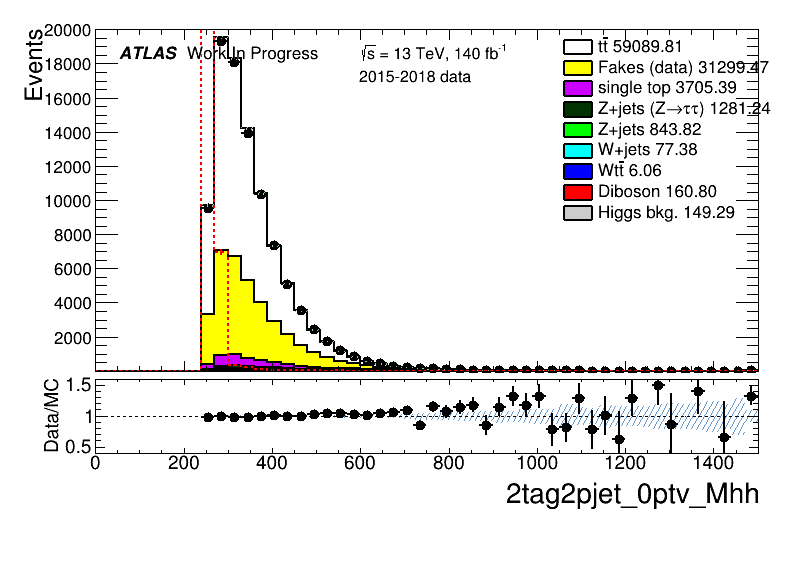
\includegraphics[width=.32\textwidth]{figures/mva/HH/LepHad/SLT/2tag2pjet_0ptv_Mhh_SR_ALLFAKES_SLT_ALL_NR_TRBins.png}
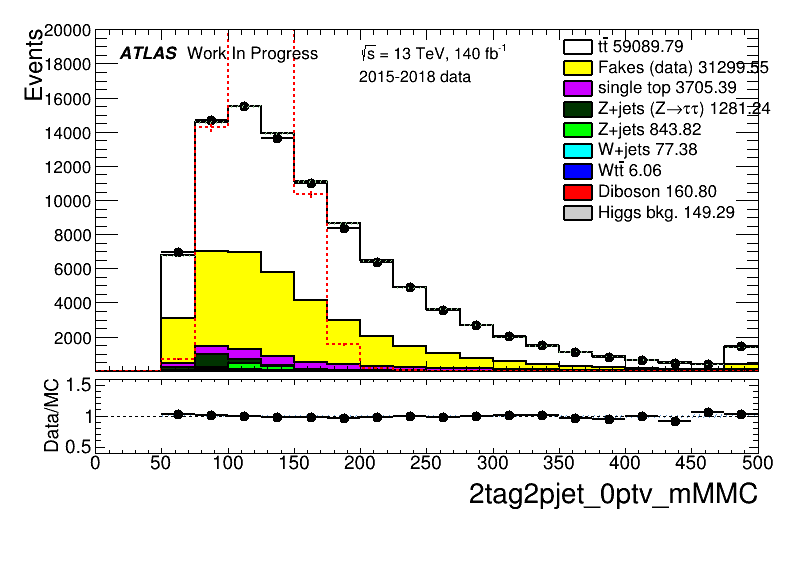
\includegraphics[width=.32\textwidth]{figures/mva/HH/LepHad/SLT/2tag2pjet_0ptv_mMMC_SR_ALLFAKES_SLT_ALL_NR_TRBins.png}
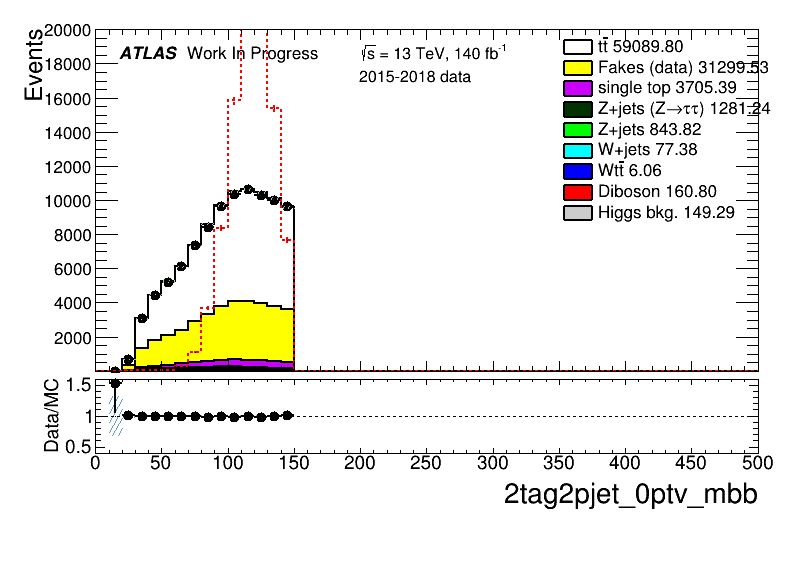
\includegraphics[width=.32\textwidth]{figures/mva/HH/LepHad/SLT/2tag2pjet_0ptv_mbb_SR_ALLFAKES_SLT_ALL_NR_TRBins.png}\\
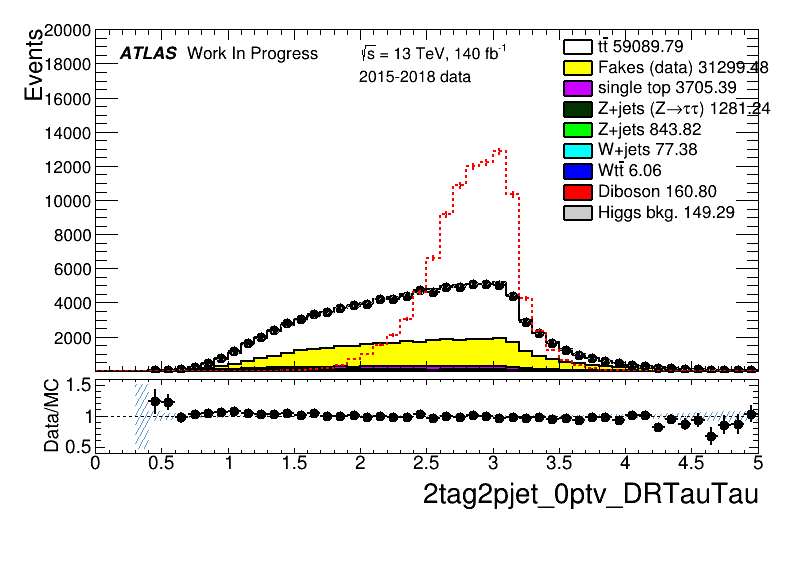
\includegraphics[width=.32\textwidth]{figures/mva/HH/LepHad/SLT/2tag2pjet_0ptv_DRTauTau_SR_ALLFAKES_SLT_ALL_NR_TRBins.png}
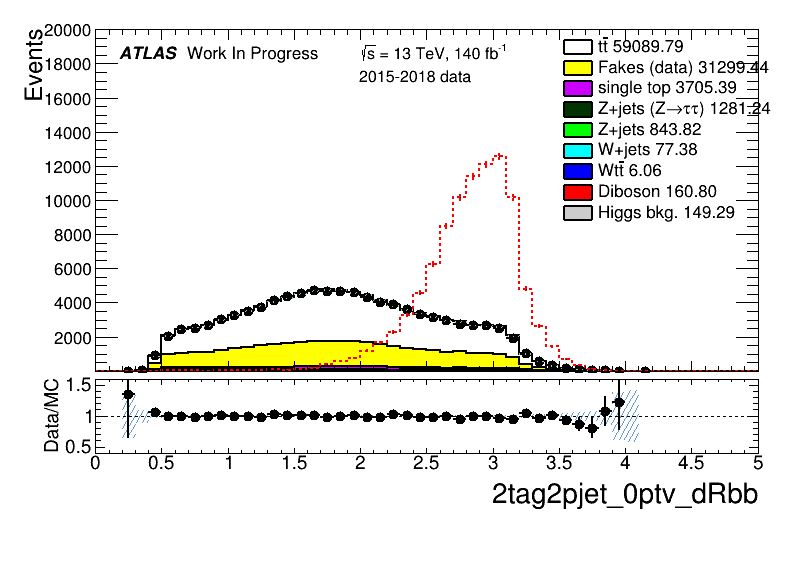
\includegraphics[width=.32\textwidth]{figures/mva/HH/LepHad/SLT/2tag2pjet_0ptv_dRbb_SR_ALLFAKES_SLT_ALL_NR_TRBins.png}
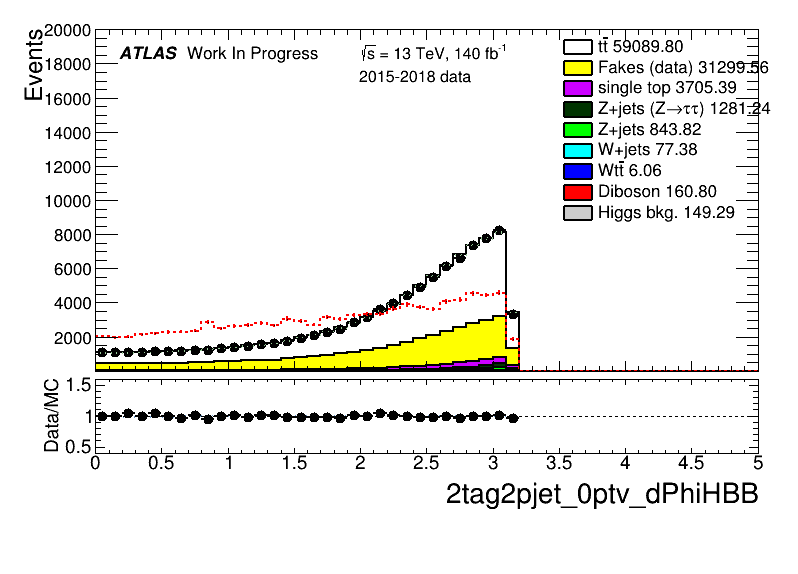
\includegraphics[width=.32\textwidth]{figures/mva/HH/LepHad/SLT/2tag2pjet_0ptv_dPhiHBB_SR_ALLFAKES_SLT_ALL_NR_TRBins.png}\\
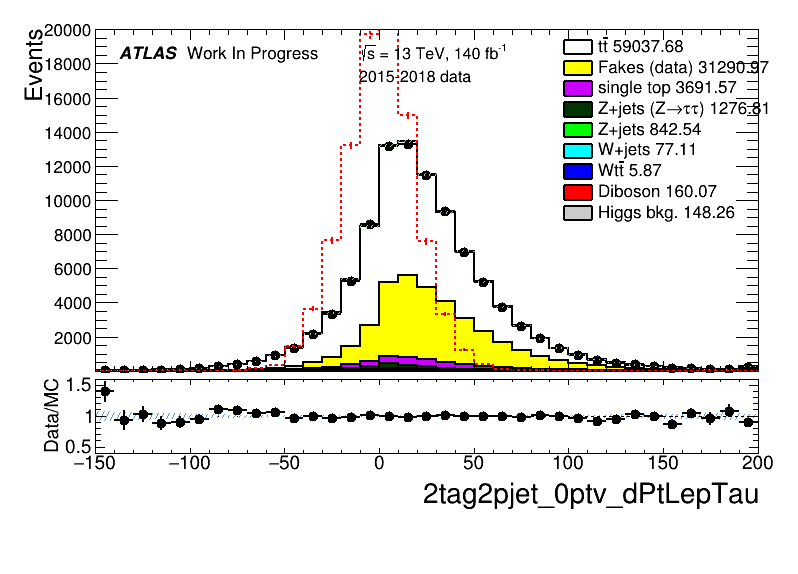
\includegraphics[width=.32\textwidth]{figures/mva/HH/LepHad/SLT/2tag2pjet_0ptv_dPtLepTau_SR_ALLFAKES_SLT_ALL_NR_TRBins.png}
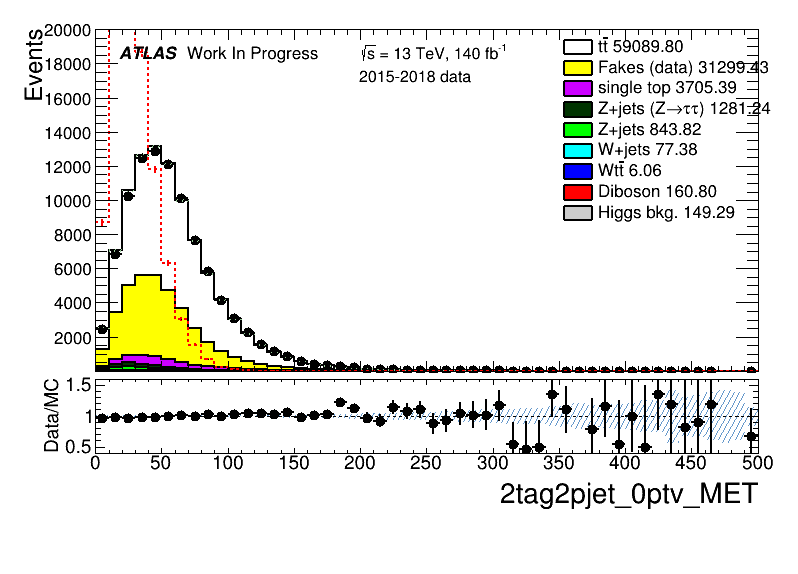
\includegraphics[width=.32\textwidth]{figures/mva/HH/LepHad/SLT/2tag2pjet_0ptv_MET_SR_ALLFAKES_SLT_ALL_NR_TRBins.png}
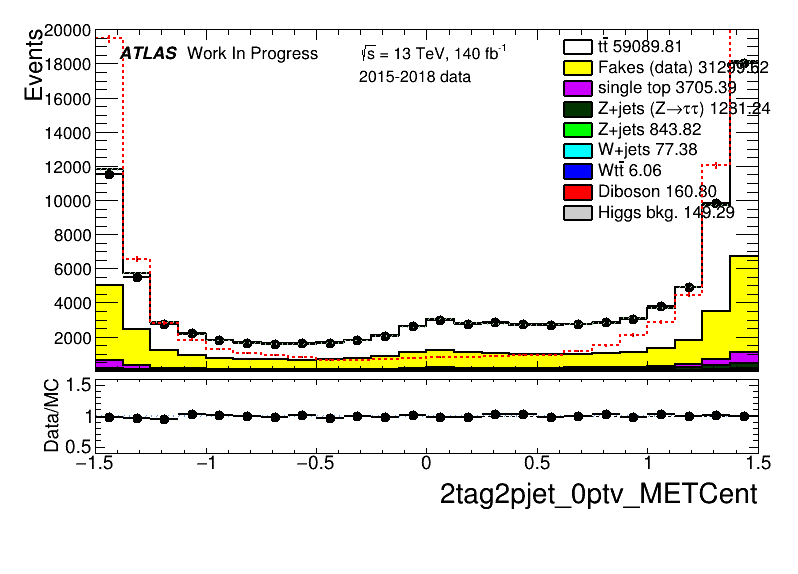
\includegraphics[width=.32\textwidth]{figures/mva/HH/LepHad/SLT/2tag2pjet_0ptv_METCent_SR_ALLFAKES_SLT_ALL_NR_TRBins.png}\\
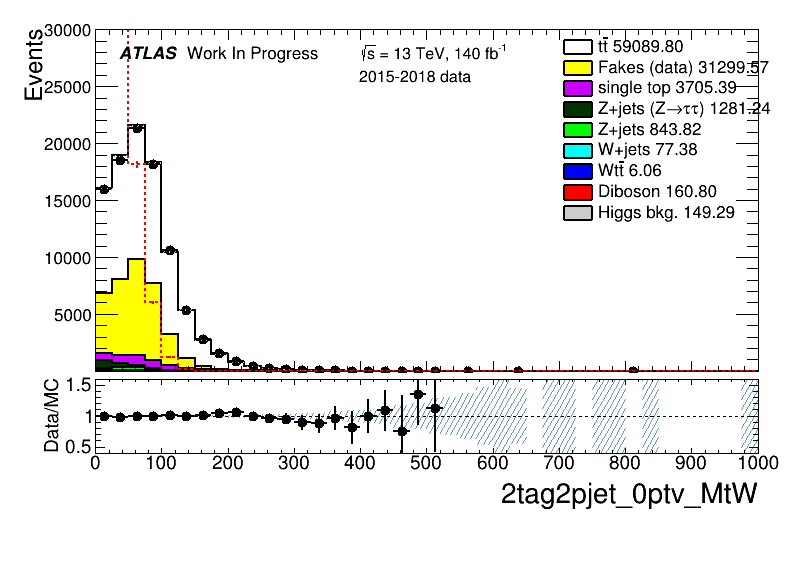
\includegraphics[width=.32\textwidth]{figures/mva/HH/LepHad/SLT/2tag2pjet_0ptv_MtW_SR_ALLFAKES_SLT_ALL_NR_TRBins.png}
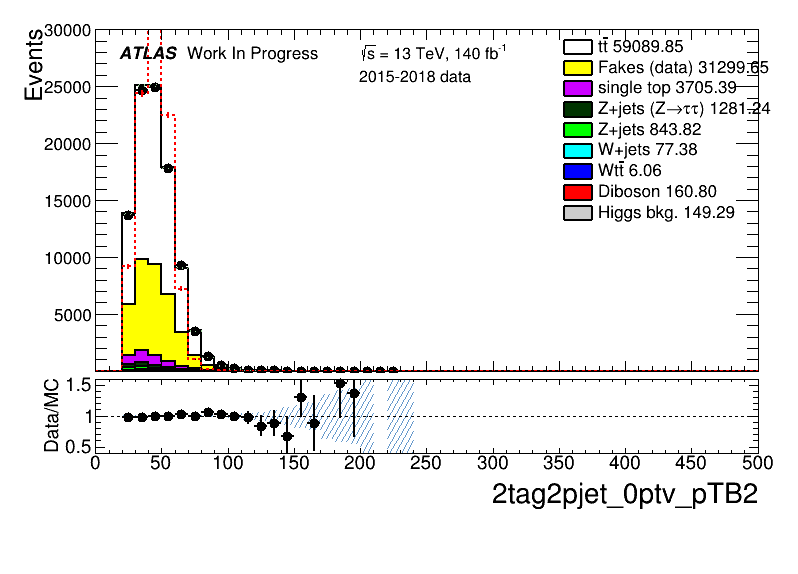
\includegraphics[width=.32\textwidth]{figures/mva/HH/LepHad/SLT/2tag2pjet_0ptv_pTB2_SR_ALLFAKES_SLT_ALL_NR_TRBins.png}
\caption{Pre-fit PNN input variable distributions in the di-Higgs $bb\lephad$ SLT signal region.}
\label{fig:lephadmvainputsslt}
\end{figure}
\fi

\begin{figure}
\centering
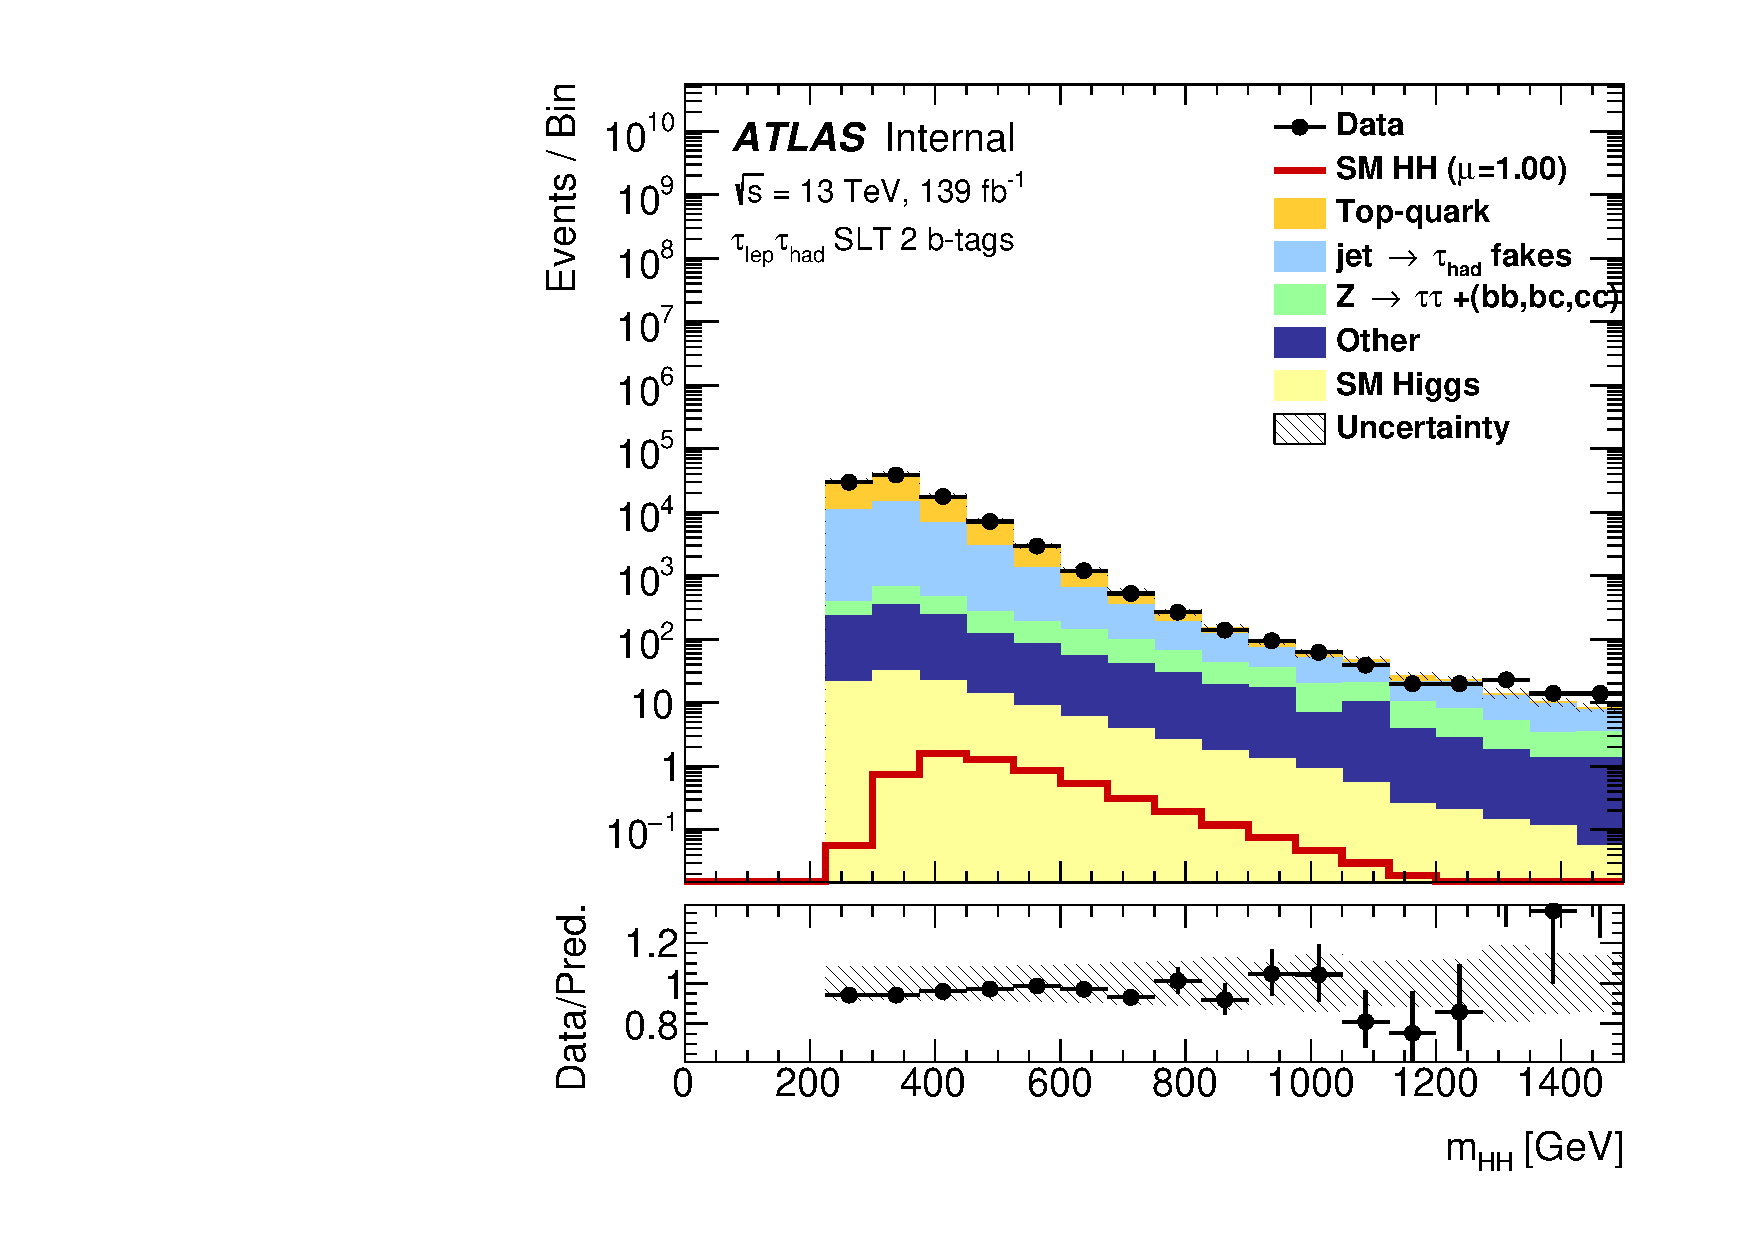
\includegraphics[width=.32\textwidth]{figures/mva/HH/LepHad/SLT/Region_BMin0_incJet1_distMhh_J2_D_T2_SpcTauLH_Y2015_LTT0_L1_Prefitlog.pdf}
\includegraphics[width=.32\textwidth]{figures/mva/HH/LepHad/SLT/Region_BMin0_incJet1_distmMMC_J2_D_T2_SpcTauLH_Y2015_LTT0_L1_Prefitlog.pdf}
\includegraphics[width=.32\textwidth]{figures/mva/HH/LepHad/SLT/Region_BMin0_incJet1_distmbb_J2_D_T2_SpcTauLH_Y2015_LTT0_L1_Prefitlog.pdf} \\
\includegraphics[width=.32\textwidth]{figures/mva/HH/LepHad/SLT/Region_BMin0_incJet1_distDRTauTau_J2_D_T2_SpcTauLH_Y2015_LTT0_L1_Prefitlog.pdf}
\includegraphics[width=.32\textwidth]{figures/mva/HH/LepHad/SLT/Region_BMin0_incJet1_distdRbb_J2_D_T2_SpcTauLH_Y2015_LTT0_L1_Prefitlog.pdf}
\includegraphics[width=.32\textwidth]{figures/mva/HH/LepHad/SLT/Region_BMin0_incJet1_distdPhiHBB_J2_D_T2_SpcTauLH_Y2015_LTT0_L1_Prefitlog.pdf} \\
\includegraphics[width=.32\textwidth]{figures/mva/HH/LepHad/SLT/Region_BMin0_incJet1_distdPtLepTau_J2_D_T2_SpcTauLH_Y2015_LTT0_L1_Prefitlog.pdf}
\includegraphics[width=.32\textwidth]{figures/mva/HH/LepHad/SLT/Region_BMin0_incJet1_distMET_J2_D_T2_SpcTauLH_Y2015_LTT0_L1_Prefitlog.pdf}
\includegraphics[width=.32\textwidth]{figures/mva/HH/LepHad/SLT/Region_BMin0_incJet1_distMETCent_J2_D_T2_SpcTauLH_Y2015_LTT0_L1_Prefitlog.pdf} \\
\includegraphics[width=.32\textwidth]{figures/mva/HH/LepHad/SLT/Region_BMin0_incJet1_distMtW_J2_D_T2_SpcTauLH_Y2015_LTT0_L1_Prefitlog.pdf}
\includegraphics[width=.32\textwidth]{figures/mva/HH/LepHad/SLT/Region_BMin0_incJet1_distpTB2_J2_D_T2_SpcTauLH_Y2015_LTT0_L1_Prefitlog.pdf}
\caption{Pre-fit PNN/NN input variable distributions in the di-Higgs $bb\lephad$ SLT signal region.}
\label{fig:lephadmvainputsslt}
\end{figure}

\iffalse
\begin{figure}
\centering
\includegraphics[width=.45\textwidth]{figures/mva/HH/LepHad/LTT/2tag2pjet_0ptv_Mhh_SR_ALLFAKES_LTT_ALL_NR_TRBins.png}
\includegraphics[width=.45\textwidth]{figures/mva/HH/LepHad/LTT/2tag2pjet_0ptv_mMMC_SR_ALLFAKES_LTT_ALL_NR_TRBins.png}\\
\includegraphics[width=.45\textwidth]{figures/mva/HH/LepHad/LTT/2tag2pjet_0ptv_mbb_SR_ALLFAKES_LTT_ALL_NR_TRBins.png}
\includegraphics[width=.45\textwidth]{figures/mva/HH/LepHad/LTT/2tag2pjet_0ptv_DRTauTau_SR_ALLFAKES_LTT_ALL_NR_TRBins.png}\\
\includegraphics[width=.45\textwidth]{figures/mva/HH/LepHad/LTT/2tag2pjet_0ptv_dPhiHttMET_SR_ALLFAKES_LTT_ALL_NR_TRBins.png}
\includegraphics[width=.45\textwidth]{figures/mva/HH/LepHad/LTT/2tag2pjet_0ptv_dPhiLep0MET_SR_ALLFAKES_LTT_ALL_NR_TRBins.png}\\
\includegraphics[width=.45\textwidth]{figures/mva/HH/LepHad/LTT/2tag2pjet_0ptv_dPtLepTau_SR_ALLFAKES_LTT_ALL_NR_TRBins.png}
\includegraphics[width=.45\textwidth]{figures/mva/HH/LepHad/LTT/2tag2pjet_0ptv_Ht_SR_ALLFAKES_LTT_ALL_NR_TRBins.png}
\caption{Pre-fit PNN input variable distributions in the di-Higgs $bb\lephad$ LTT signal region.}
\label{fig:lephadmvainputsltt}
\end{figure}
\fi

\begin{figure}
\centering
\includegraphics[width=.32\textwidth]{figures/mva/HH/LepHad/LTT/Region_BMin0_incJet1_distMhh_J2_D_T2_SpcTauLH_Y2015_LTT1_L1_Prefitlog.pdf}
\includegraphics[width=.32\textwidth]{figures/mva/HH/LepHad/LTT/Region_BMin0_incJet1_distmMMC_J2_D_T2_SpcTauLH_Y2015_LTT1_L1_Prefitlog.pdf} 
\includegraphics[width=.32\textwidth]{figures/mva/HH/LepHad/LTT/Region_BMin0_incJet1_distmbb_J2_D_T2_SpcTauLH_Y2015_LTT1_L1_Prefitlog.pdf} \\
\includegraphics[width=.32\textwidth]{figures/mva/HH/LepHad/LTT/Region_BMin0_incJet1_distDRTauTau_J2_D_T2_SpcTauLH_Y2015_LTT1_L1_Prefitlog.pdf} 
\includegraphics[width=.32\textwidth]{figures/mva/HH/LepHad/LTT/Region_BMin0_incJet1_distdPhiHttMET_J2_D_T2_SpcTauLH_Y2015_LTT1_L1_Prefitlog.pdf}
\includegraphics[width=.32\textwidth]{figures/mva/HH/LepHad/LTT/Region_BMin0_incJet1_distdPhiLep0MET_J2_D_T2_SpcTauLH_Y2015_LTT1_L1_Prefitlog.pdf} \\
\includegraphics[width=.32\textwidth]{figures/mva/HH/LepHad/LTT/Region_BMin0_incJet1_distdPtLepTau_J2_D_T2_SpcTauLH_Y2015_LTT1_L1_Prefitlog.pdf}
\includegraphics[width=.32\textwidth]{figures/mva/HH/LepHad/LTT/Region_BMin0_incJet1_distHt_J2_D_T2_SpcTauLH_Y2015_LTT1_L1_Prefitlog.pdf}
\caption{Pre-fit PNN/NN input variable distributions in the di-Higgs $bb\lephad$ LTT signal region.}
\label{fig:lephadmvainputsltt}
\end{figure}

\begin{figure}
\centering
\includegraphics[width=.32\textwidth]{figures/mva/HH/LepHad/SLT/Region_BMin0_incJet1_dist300_J2_D2HDMPNN_T1_SpcTauLH_Y2015_LTT0_L1_Prefitlog.pdf}
\includegraphics[width=.32\textwidth]{figures/mva/HH/LepHad/SLT/Region_BMin0_incJet1_dist500_J2_D2HDMPNN_T1_SpcTauLH_Y2015_LTT0_L1_Prefitlog.pdf}
\includegraphics[width=.32\textwidth]{figures/mva/HH/LepHad/SLT/Region_BMin0_incJet1_dist1000_J2_D2HDMPNN_T1_SpcTauLH_Y2015_LTT0_L1_Prefitlog.pdf} \\
\includegraphics[width=.32\textwidth]{figures/mva/HH/LepHad/SLT/Region_BMin0_incJet1_dist1600_J2_D2HDMPNN_T1_SpcTauLH_Y2015_LTT0_L1_Prefitlog.pdf}
\includegraphics[width=.32\textwidth]{figures/mva/HH/LepHad/SLT/Region_BMin0_incJet1_distNN_J2_DSM_T1_SpcTauLH_Y2015_LTT0_L1_Prefitlog.pdf} \\
\includegraphics[width=.32\textwidth]{figures/mva/HH/LepHad/LTT/Region_BMin0_incJet1_dist300_J2_D2HDMPNN_T1_SpcTauLH_Y2015_LTT1_L1_Prefitlog.pdf}
\includegraphics[width=.32\textwidth]{figures/mva/HH/LepHad/LTT/Region_BMin0_incJet1_dist500_J2_D2HDMPNN_T1_SpcTauLH_Y2015_LTT1_L1_Prefitlog.pdf}
\includegraphics[width=.32\textwidth]{figures/mva/HH/LepHad/LTT/Region_BMin0_incJet1_dist1000_J2_D2HDMPNN_T1_SpcTauLH_Y2015_LTT1_L1_Prefitlog.pdf} \\
\includegraphics[width=.32\textwidth]{figures/mva/HH/LepHad/LTT/Region_BMin0_incJet1_dist1600_J2_D2HDMPNN_T1_SpcTauLH_Y2015_LTT1_L1_Prefitlog.pdf}
\includegraphics[width=.32\textwidth]{figures/mva/HH/LepHad/LTT/Region_BMin0_incJet1_distNN_J2_DSM_T1_SpcTauLH_Y2015_LTT1_L1_Prefitlog.pdf}
\caption{Pre-fit PNN score distributions for the $300, 500, 1000, 1600$ GeV mass points and non-resonant NN in the di-Higgs $bb\lephad$ SLT (top two rows) and LTT (bottom two rows) 1tag control regions.}
\label{fig:lephadmvaCRoutput}
\end{figure}
 
\begin{figure}
\centering
\includegraphics[width=.32\textwidth]{figures/mva/HH/LepHad/SLT/Region_BMin0_incJet1_dist300_J2_D2HDMPNN_T2_SpcTauLH_Y2015_LTT0_L1_Prefitlog.pdf}
\includegraphics[width=.32\textwidth]{figures/mva/HH/LepHad/SLT/Region_BMin0_incJet1_dist500_J2_D2HDMPNN_T2_SpcTauLH_Y2015_LTT0_L1_Prefitlog.pdf}
\includegraphics[width=.32\textwidth]{figures/mva/HH/LepHad/SLT/Region_BMin0_incJet1_dist1000_J2_D2HDMPNN_T2_SpcTauLH_Y2015_LTT0_L1_Prefitlog.pdf} \\
\includegraphics[width=.32\textwidth]{figures/mva/HH/LepHad/SLT/Region_BMin0_incJet1_dist1600_J2_D2HDMPNN_T2_SpcTauLH_Y2015_LTT0_L1_Prefitlog.pdf} 
\includegraphics[width=.32\textwidth]{figures/mva/HH/LepHad/SLT/Region_BMin0_incJet1_distNN_J2_DSM_T2_SpcTauLH_Y2015_LTT0_L1_Prefitlog.pdf} \\
\includegraphics[width=.32\textwidth]{figures/mva/HH/LepHad/LTT/Region_BMin0_incJet1_dist300_J2_D2HDMPNN_T2_SpcTauLH_Y2015_LTT1_L1_Prefitlog.pdf}
\includegraphics[width=.32\textwidth]{figures/mva/HH/LepHad/LTT/Region_BMin0_incJet1_dist500_J2_D2HDMPNN_T2_SpcTauLH_Y2015_LTT1_L1_Prefitlog.pdf}
\includegraphics[width=.32\textwidth]{figures/mva/HH/LepHad/LTT/Region_BMin0_incJet1_dist1000_J2_D2HDMPNN_T2_SpcTauLH_Y2015_LTT1_L1_Prefitlog.pdf} \\
\includegraphics[width=.32\textwidth]{figures/mva/HH/LepHad/LTT/Region_BMin0_incJet1_dist1600_J2_D2HDMPNN_T2_SpcTauLH_Y2015_LTT1_L1_Prefitlog.pdf} 
\includegraphics[width=.32\textwidth]{figures/mva/HH/LepHad/LTT/Region_BMin0_incJet1_distNN_J2_DSM_T2_SpcTauLH_Y2015_LTT1_L1_Prefitlog.pdf}
\caption{Pre-fit PNN score distributions for the $300, 500, 1000, 1600$ GeV mass points and non-resonant NN in the di-Higgs $bb\lephad$ SLT (top two rows) and LTT (bottom two rows) signal regions.}
\label{fig:lephadmvaoutput}
\end{figure}


%To validate the ability of the combined fake factor method to describe the PNN or NN shape, plots have been made using the fake factor method to estimate the 
%combined multi-jet and $t\bar{t}/W$ contribution in validation regions. First, we have applied the combined fake factor method directly to the $\ttbar$ CR, as a 
%closure test of the method, which can be seen in Fig.~\ref{fig:ttCR_val}. The next region is the high statistic and relatively background-enriched $0$-tag region, 
%which is the same as the lephad signal region except for the requirement that there are no $b$-tagged jets.  This is shown in Fig.~\ref{fig:SLT_0tag} and 
%Fig.~\ref{fig:LTT_0tag} for several mass hypotheses and for the single lepton and lepton-plus-tau trigger categories, respectively. In Fig.~\ref{fig:SLT_LTT_1tag}, a 
%few distributions are also shown for a validation region closer to the signal region, the $1$-tag validation region, which requires the same selection as the signal 
%region with the exception of requiring exactly one $b$-tagged jet. The background estimation appears to agree well with the observed distributions in these 
%validation regions.

To validate the modeling, we have also included distributions of the PNN inputs for the 400 GeV PNN discriminant $>0.5$ for the 
0-tag and 1-tag validation regions. The plots can be found in 
\cref{subsec:appendix_bkg_validation_lephad}, \cref{fig:lephadmvainputsslt_0tag,fig:lephadmvainputsltt_0tag,fig:lephadmvainputsslt_1tag,fig:lephadmvainputsltt_1tag}.

\clearpage

\label{sec:mva_hh}

\subsection{Leptoquark}
\label{sec:mva_lq}
Parametric Neural Networks (PNNs) are used as for the di-Higgs analysis to separate the signal from the expected backgrounds, and the PNN score distributions are final discriminant in the fit. Events are required to pass their respective selection criteria described in~\Cref{subsec:sellq_lephad},~\ref{subsec:sellq_hadhad} and the MC samples are weighted by their predicted cross sections.  The hyper parameters used for training used are summarised in~\Cref{tab:hyper_parameters_PNN_LQ}. In the~\Cref{sec:appendix_pnn}, studies on the input samples, hyper parameter optimization, signal statistics, and the over training checks are shown.

\FloatBarrier

\begin{table}
\centering
\small
\begin{tabular}{|c|c|}
\hline
Parameter & Value\\
\hline
Epochs & 100\\
Batch-size & 64\\
Learning rate & 0.1\\
Learning rate decay & 1e-5\\
Nesterov momentum & 0.9 \\
Layer sizes & 32 32 32\\
\hline
\end{tabular}
\caption{Training hyper parameters used for the LQLQ PNNs.}
\label{tab:hyper_parameters_PNN_LQ}
\end{table}

\subsubsection{\lephad}
The training is performed against the dominant \ttbar background with the real and fake tau components both taken from the MC simulation.
The input variables used to provide good discrimination between signal and background are:
\begin{itemize}
    \item $\Delta R(\ell,jet)$: the $\Delta R$ between the lepton and jet
    \item $\Delta \phi(\ell,E_{T}^{\mathrm{miss}})$: the opening angle between the light-lepton and the missing energy
    \item $s_{T}$ : the scalar sum of $E_{T}^{\mathrm{miss}}$, the $p_{T}$ of taus, two highest jets and lepton
    \item $E_{T}^{\mathrm{miss}} \phi$ centrality: the position in $\phi$ of $E_{T}^{\mathrm{miss}}$ between taus
    \item $m_{\tau,jet}$: the invariant mass between hadronic tau and its paired jet
    \item $m_{\ell,jet}$: the invariant mass between light-lepton and its paired jet
    \item \tauhad $p_T$
\end{itemize}

Input variable distributions are shown in Fig.~\ref{fig:PNN_input_lephad} for 1+2-$b$-tag signal region. The PNN score distributions
are shown in Fig.~\ref{fig:PNN_lephad}.

\begin{figure}
    \centering
    \subfloat[]{ \includegraphics[width=0.3\textwidth]{figures/mva/lq3/lephad/FinalPlots_TauLH_SR_cluster1_btag77_fullrun2_20210217_BasicKinematics_OS_combined_METCentrality_Rebin10.pdf}}
    \subfloat[]{ \includegraphics[width=0.3\textwidth]{figures/mva/lq3/lephad/FinalPlots_TauLH_SR_cluster1_btag77_fullrun2_20210217_BasicKinematics_OS_combined_m_LQ_had_Rebin25.pdf}}
    \subfloat[]{ \includegraphics[width=0.3\textwidth]{figures/mva/lq3/lephad/FinalPlots_TauLH_SR_cluster1_btag77_fullrun2_20210217_BasicKinematics_OS_combined_m_LQ_lep_Rebin25.pdf}}\\
    \subfloat[]{ \includegraphics[width=0.3\textwidth]{figures/mva/lq3/lephad/FinalPlots_TauLH_SR_cluster1_btag77_fullrun2_20210217_BasicKinematics_OS_combined_Tau0Pt_Rebin10.pdf}}
    \subfloat[]{ \includegraphics[width=0.3\textwidth]{figures/mva/lq3/lephad/FinalPlots_TauLH_SR_cluster1_btag77_fullrun2_20210217_BasicKinematics_OS_combined_dPhi_LepMET_Rebin15.pdf}}
    \subfloat[]{ \includegraphics[width=0.3\textwidth]{figures/mva/lq3/lephad/FinalPlots_TauLH_SR_cluster1_btag77_fullrun2_20210217_BasicKinematics_OS_combined_dR_J0Lep_Rebin20.pdf}}\\
    \subfloat[]{ \includegraphics[width=0.3\textwidth]{figures/mva/lq3/lephad/FinalPlots_TauLH_SR_cluster1_btag77_fullrun2_20210217_BasicKinematics_OS_combined_sT_Rebin40.pdf}}
    \caption{ 
     The pre-fit PNN input variable distributions in the LQLQ \lephad signal region. 
%     As discussed in the Sec~\ref{subsec:sellq_lephad}, these distributions include 1- and 2-$b$-tag events.
%     The red coloured line shows the LQ \lephad signal yields ($m=1100$ GeV).
    }
   \label{fig:PNN_input_lephad}
\end{figure}

\begin{figure}
    \centering
    \subfloat[]{ \includegraphics[width=0.3\textwidth]{figures/mva/lq3/lephad/Region_BMin0_incJet1_dist300_J2_Dbeta1p0PNN_T2_SpcTauLH_Y2015_LTT0_L1_Prefitlog.pdf}}
    \subfloat[]{ \includegraphics[width=0.3\textwidth]{figures/mva/lq3/lephad/Region_BMin0_incJet1_dist500_J2_Dbeta1p0PNN_T2_SpcTauLH_Y2015_LTT0_L1_Prefitlog.pdf}}
    \subfloat[]{ \includegraphics[width=0.3\textwidth]{figures/mva/lq3/lephad/Region_BMin0_incJet1_dist900_J2_Dbeta1p0PNN_T2_SpcTauLH_Y2015_LTT0_L1_Prefitlog.pdf}} \\
    \subfloat[]{ \includegraphics[width=0.3\textwidth]{figures/mva/lq3/lephad/Region_BMin0_incJet1_dist1000_J2_Dbeta1p0PNN_T2_SpcTauLH_Y2015_LTT0_L1_Prefitlog.pdf}}
    \subfloat[]{ \includegraphics[width=0.3\textwidth]{figures/mva/lq3/lephad/Region_BMin0_incJet1_dist1100_J2_Dbeta1p0PNN_T2_SpcTauLH_Y2015_LTT0_L1_Prefitlog.pdf}}
    \subfloat[]{ \includegraphics[width=0.3\textwidth]{figures/mva/lq3/lephad/Region_BMin0_incJet1_dist1200_J2_Dbeta1p0PNN_T2_SpcTauLH_Y2015_LTT0_L1_Prefitlog.pdf}} \\
    \subfloat[]{ \includegraphics[width=0.3\textwidth]{figures/mva/lq3/lephad/Region_BMin0_incJet1_dist1300_J2_Dbeta1p0PNN_T2_SpcTauLH_Y2015_LTT0_L1_Prefitlog.pdf}}
    \subfloat[]{ \includegraphics[width=0.3\textwidth]{figures/mva/lq3/lephad/Region_BMin0_incJet1_dist1400_J2_Dbeta1p0PNN_T2_SpcTauLH_Y2015_LTT0_L1_Prefitlog.pdf}}
    \subfloat[]{ \includegraphics[width=0.3\textwidth]{figures/mva/lq3/lephad/Region_BMin0_incJet1_dist1500_J2_Dbeta1p0PNN_T2_SpcTauLH_Y2015_LTT0_L1_Prefitlog.pdf}} \\

    \caption{ 
      The pre-fit PNN distributions in the LQLQ \lephad signal region.  
%     As discussed in the Sec~\ref{subsec:sellq_lephad}, these distributions include 1- and 2-$b$-tag events.
      The red coloured line shows the LQ \lephad signal yields for the corresponding mass point.
    }
         \label{fig:PNN_lephad}
\end{figure}

\subsubsection{\hadhad}
The training is performed against the dominant \ttbar background. The contribution of other backgrounds is small with respect to \ttbar events as shown in~\Cref{tab:LQHadHadYields}. The input variables chosen to provide a good discrimination between signal and background are:
\begin{itemize}
    \item $p_{T\tau 0}$: $p_T$ of the leading $\tau$
    \item ${\eta_{\tau 0}}$: $\eta$ of the leading $\tau$
    \item $m_{LQ0,1}$: the masses reconstructed from $b$ and $\tau$ which are paired by $\mathrm{min}|\Delta m|$ method described in~\Cref{subsec:btau_pairing}. The masses of both combination are used as input
    \item $\Delta R(\tau, jet)$: $\Delta R$ between the leading $\tau$ and the jet
    \item $E_{T}^{\mathrm{miss}} \phi$ centrality: the position in $\phi$ of $E_{T}^{\mathrm{miss}}$ between $\tau$'s
    \item $s_{T}$: the scalar sum of $E_{T}^{\mathrm{miss}}$, the $p_{T}$ of two $\tau$'s and two highest jets
\end{itemize}

Input variables distributions are shown in~\Cref{fig:PNN_input_hadhad}. The PNN score distributions are shown in~\Cref{fig:PNN_hadhad}.

\begin{figure}[]
    \centering
    \subfloat[]{ \includegraphics[width=0.4\textwidth]{figures/selection/lq3/hadhad/Plots_SR/C_3tag2pjet_0ptv_OS_Tau0Pt.eps}}
    \subfloat[]{ \includegraphics[width=0.4\textwidth]{figures/selection/lq3/hadhad/Plots_SR/C_3tag2pjet_0ptv_OS_Tau0Eta.eps}} \\
    \subfloat[]{ \includegraphics[width=0.4\textwidth]{figures/mva/lq3/hadhad/C_3tag2pjet_0ptv_OS_SR_sT.eps}}
    \subfloat[]{ \includegraphics[width=0.4\textwidth]{figures/mva/lq3/hadhad/C_3tag2pjet_0ptv_OS_SR_METCent.eps}} \\
    \subfloat[]{ \includegraphics[width=0.4\textwidth]{figures/mva/lq3/hadhad/C_3tag2pjet_0ptv_OS_SR_m_LQ0.eps}} 
    \subfloat[]{ \includegraphics[width=0.4\textwidth]{figures/mva/lq3/hadhad/C_3tag2pjet_0ptv_OS_SR_m_LQ1.eps}} \\
    \subfloat[]{ \includegraphics[width=0.4\textwidth]{figures/mva/lq3/hadhad/C_3tag2pjet_0ptv_OS_SR_DRTauJetLQ.eps}}
    \caption{ 
     The pre-fit PNN input variable distributions in the LQLQ \hadhad signal region. The red coloured line shows the LQ \hadhad signal yields ($m=1100$ GeV).
    }
     \label{fig:PNN_input_hadhad}
\end{figure}



\begin{figure}
    \centering
    \subfloat[]{ \includegraphics[width=0.4\textwidth]{figures/mva/lq3/hadhad/prefit_PNN/Region_BMin0_incJet1_dist500_J2_Y2015_DOSSRLQ3PNN0_T3_SpcTauHH_L0_Prefitlog.pdf}}
    \subfloat[]{ \includegraphics[width=0.4\textwidth]{figures/mva/lq3/hadhad/prefit_PNN/Region_BMin0_incJet1_dist800_J2_Y2015_DOSSRLQ3PNN0_T3_SpcTauHH_L0_Prefitlog.pdf}} \\
    \subfloat[]{ \includegraphics[width=0.4\textwidth]{figures/mva/lq3/hadhad/prefit_PNN/Region_BMin0_incJet1_dist1000_J2_Y2015_DOSSRLQ3PNN0_T3_SpcTauHH_L0_Prefitlog.pdf}}
    \subfloat[]{ \includegraphics[width=0.4\textwidth]{figures/mva/lq3/hadhad/prefit_PNN/Region_BMin0_incJet1_dist1200_J2_Y2015_DOSSRLQ3PNN0_T3_SpcTauHH_L0_Prefitlog.pdf}} \\
    \subfloat[]{ \includegraphics[width=0.4\textwidth]{figures/mva/lq3/hadhad/prefit_PNN/Region_BMin0_incJet1_dist1400_J2_Y2015_DOSSRLQ3PNN0_T3_SpcTauHH_L0_Prefitlog.pdf}}
    \subfloat[]{ \includegraphics[width=0.4\textwidth]{figures/mva/lq3/hadhad/prefit_PNN/Region_BMin0_incJet1_dist1600_J2_Y2015_DOSSRLQ3PNN0_T3_SpcTauHH_L0_Prefitlog.pdf}} \\
    \caption{ 
     The pre-fit PNN distributions in the LQLQ \hadhad signal region. The red coloured line shows the LQ \hadhad signal yields.
    }
     \label{fig:PNN_hadhad}
\end{figure}

\FloatBarrier

\label{sec:mva_lq}
